\documentclass[runningheads]{jblab}

\usepackage[utf8]{inputenc}
\usepackage[english,russian]{babel}
\usepackage[T2A]{fontenc}
\usepackage{amsmath}
\usepackage{indentfirst}
\usepackage{amsfonts}
\usepackage{amssymb}
\usepackage{graphicx}
\usepackage{listings}
\usepackage{algpseudocode}
\usepackage{algorithm}
\usepackage{caption}
\usepackage{algorithmicx}
\usepackage{wrapfig}
\usepackage{supertabular}
\usepackage{epigraph}
\usepackage{euscript}
\usepackage{textcomp}
\usepackage{cite}
\usepackage{ucs}
\usepackage[caption=false]{subfig}

\pdfpagewidth=14.8cm
\pdfpageheight=21cm

\textwidth=10cm
\textheight=15cm

\oddsidemargin=0pt
\evensidemargin=0pt

\topmargin=0pt


\begin{document}

\newcommand{\Issue}[0]{1}
\newcommand{\Year}[0]{2013}
\sloppy

\begin{titlepage}

\centering


\includegraphics[width=4cm]{JBLogoWhite.png}
\vskip 2cm
\mbox{\Large{\textsc{Труды лаборатории}}}
\vskip 0.5cm
\mbox{\Large{\textsc{языковых инструментов}}}
%\vskip 0.5cm
%<\mbox{\Large{\textsc{компании JetBrains}}}
\vskip 2.5cm
\large{Выпуск \Issue}
\vskip 6cm
\large{Санкт-Петербург, \Year}
\end{titlepage}

\thispagestyle{empty}
\phantom{xx}
\pagebreak

\chapter*{Предисловие}

В октябре 2012 года компания JetBrains --- один из мировых лидеров в области 
производства средств поддержки разработки ПО --- анонсировала создание на
математико-механическом факультете Санкт-Петербургского государственного университета
лаборатории языковых инструментов. Задачей этой лаборатории является реализация
силами студентов и аспирантов факультета научно-исследовательских и образовательных 
проектов в областях компетенции компании.

Настоящий сборник представляет работы, выполненные студентами лаборатории в 2012-2013 учебном году.
Среди тем этих работ можно найти как классические, такие как управление памятью и сборка 
мусора, декомпиляция, форматирование исходных текстов, так и сравнительно 
новые направления, связанные с сертификационным программированием и анализом 
встроенных языков.

Следует отметить, что все представленные работы были не только проведены в лаборатории 
под руководством специалистов JetBrains, но и засчитаны их авторам 
в качестве курсовых или дипломных работ. 
\vskip 2cm
\begin{flushright}
\textit{куратор лаборатории Д.Булычев}
\end{flushright}

\tableofcontents

%\documentclass[12pt,a4paper]{article}
%\usepackage[utf8x]{inputenc}
%\usepackage[russian]{babel}
%\usepackage[OT1]{fontenc}
%\usepackage{amsmath}
%\usepackage[a4paper,includeheadfoot,top=20mm,bottom=20mm,left=25mm,right=15mm]{geometry}
%\usepackage{indentfirst}
%\usepackage{amsfonts}
%\usepackage{amssymb}
%\usepackage{graphicx}
%\renewcommand\baselinestretch{1.5}
%\renewcommand\contentsname{Оглавление}

%\begin{document}
%\begin{titlepage}
%\thispagestyle{empty}
%\def\baselinestretch{1.0}
%\begin{center}
%	{\large САНКТ-ПЕТЕРБУРГСКИЙ ГОСУДАРСТВЕННЫЙ УНИВЕРСИТЕТ \\ \vskip 0.3em {\large Математико-механический факультет \\ \vskip 0.7em{\large Кафедра системного программирования \\}}}
%    \vspace*{0.15\textheight}
%    \vfill
%    {\large Шашкова Елизавета Михайловна}
%    
%    \vskip 2em
%    {\huge Методы профилирования реализаций кучи}
%    
%    \vskip 1em
%    {\large Курсовая работа} \\
%    \vskip 2em
%    {\normalsize \raggedleft 
%    Научный руководитель:\\
%    к.ф.-м.н. Д.Ю. Булычев
%    \\[3em]
%    \vspace*{0.08\textheight}
%    \vfill
%    {\centering Санкт-Петербург \\ 2013}
%    }
%\end{center}
%\end{titlepage}

\title{Методы профилирования реализаций кучи}
%
\titlerunning{Методы профилирования реализаций кучи}
\author{Шашкова Елизавета Михайловна}
%
\authorrunning{Е.М.Шашкова} % abbreviated author list (for running head)
%
%%%% list of authors for the TOC (use if author list has to be modified)
\tocauthor{Е.М.Шашкова}
%
\institute{Санк-Петербургский государственный университет\\
\email{Elizaveta239@yandex.ru}}

\maketitle              % typeset the title of the contribution

\begin{abstract}
\end{abstract}
%

\section*{Введение}

   Динамическое управление памятью --- это управление памятью для объектов, ни размер, ни время жизни которых, вообще говоря, неизвестны до
   выполнения программы. Под объектом мы будем понимать некоторый неделимый набор байт.
   
   Обычно при динамическом управлении памятью место под объекты выделяется в специальной области памяти --- \textquotedblleft куче\textquotedblright
   (heap). Существует
   две основных операции для управления памятью в куче: выделение памяти и освобождение. При выделении посылается запрос, в котором указывается количество
   требуемой памяти. При успешном выделении память изымается из кучи, то есть становится недоступна для последующего выделения.
   Освобождение памяти, наоборот, делает часть кучи доступной для последующего выделения.
   
   Поведение динамической памяти удобно описывать в терминах взаимодействия двух основных сущностей: \emph{аллокатора} и \emph{мутатора}. Аллокатор принимает запросы на выделение
   памяти в куче и её освобождение. Мутатор посылает данные запросы. Каждый запрос содержит количество памяти для выделения, причем 
   это количество, вообще говоря, становится известно только в момент исполнения программы.
   
   Эффективность работы программы во многом зависит от эффективности аллокатора. На сегодняшний момент существует много способов его 
   реализации; более того, развитие технологий стимулирует создание новых подходов. Поэтому становится важной задача уметь сравнивать разные
   реализации аллокаторов, находить наиболее подходящие реализации в данном конкретном случае.
   
   Для описания свойств аллокатора можно выделить два полярных подхода:
   \begin{enumerate}
   \item Рассмотрение свойств кучи с точки зрения поведения мутатора. Задача: определить, для какого класса программ данная реализация аллокатора 
   подойдет лучше всего. 
   \item Сравнительный анализ нескольких реализаций аллокатора. Задача: провести сравнение двух или нескольких аллокаторов при взаимодействии с
   одним и тем же мутатором.
   \end{enumerate}
   
   Основные свойства, которыми можно описать аллокатор в первом подходе:
   \begin{itemize}
   \item Суммарное количество выделенной памяти (в байтах и блоках).
   \item Наибольшее количество единовременно выделенной памяти за все время работы программы (в байтах и блоках).
   \item Среднее время жизни блока (в байтах). Это время вычисляется, как количество байт, помещенных в кучу за промежуток времени между 
   созданием и удалением объекта, поделенное на размер объекта (среднее время жизни одного байта в куче).
   \end{itemize}
   
   Основные свойства, которыми можно описать аллокатор во втором подходе:
   \begin{itemize}
   \item Фрагментация. Фрагментация вычисляется по следующей формуле: \[ F = \frac{free - free_{max}}{free} \]
   где $free$ --- количество свободных байт в куче, $free_{max}$ --- размер (в байтах) наибольшего свободного блока.  Так как память в куче выделяется
   блоками (наборами байтов), может так случиться, что в куче не осталось места для блока требуемого размера, хотя количество свободной 
   памяти еще превышает размер этого блока. С помощью данной формулы фрагментацию можно описать численной величиной. Чем меньше эта
   величина, тем \textquotedblleft лучше\textquotedblright~текущее состояние кучи. Фрагментации равна нулю, когда свободное место в 
   куче является одним блоком, и приближается к единице, когда размеры всех свободных блоков в куче малы. 
   \item Время выделения (в единицах времени).
   \item Порог работоспособности (количество запросов, обработанных аллокатором).
   \item Зависимость скорости работы аллокатора от нагрузки.
   \end{itemize}
    
   Цель данной курсовой работы заключается в том, чтобы изучить методы оценки реализации аллокатора. Необходимо понять, насколько 
   эффективно использование того или иного аллокатора, определить критерии, по которым различные аллокаторы будут сравниваться. В 
   соответствии с основными подходами, нужно сравнить поведение одного аллокатора при использовании нескольких различных мутаторов, а также
   сравнить поведение нескольких аллокаторов при работе с одним мутатором. В результате будет создан прототип системы для проведения 
   вышеуказанных сравнений.
   
   
   \section{Существующие подходы и метрики}
   Для сравнения различных реализаций аллокаторов прежде всего нужно выбрать метрики, по которым будет 
   производиться сравнение. Требуется понять, какие данные нужно собирать при запуске программ
   с использованием различных аллокаторов.
   
   В статье ~\cite{six_progs} представлены опытные данные, полученные с помощью шести программ на языке
   C. Авторы запустили каждую программу на нескольких наборах входных данных и построили распределения для следующих величин:
   
   \begin{itemize}
   \item размеров объектов;
   \item времён жизни объектов;
   \item интервалов времени между запросами.
   \end{itemize}
   
   Для этих распределений были найдены среднее, медиана и мода, которые характеризуют асимметричность распределения. Распределение размеров 
   объектов оказалось асимметричным 
   в сторону маленьких размеров: большая часть объектов, под которые выделялась память, имели размер менее 64 байт. Интересным
   оказался тот факт, что 90\% объектов имеют всего 10 различных размеров. Распределение времени жизни
   объектов показало, что большинство объектов живет в течение короткого промежутка времени: 40-80 машинных инструкций процессора 
   
   Данные об использовании памяти были получены посредством трассировки с помощью методики abstract execution~\cite{ae}. В качестве 
   тестовых программ для измерения были взяты: программа, находящая факториал больших целых чисел; оптимизатор Espresso; 
   GhostScript\footnote{http://www.ghostscript.com/} –-- интерпретатор языка PostScript; Gnu Awk\footnote{http://www.gnu.org/software/gawk/} –-- 
   интерпретатор языка AWK; интерпретатор Perl\footnote{http://www.perl.org/}; Chameleon –-- канальный роутер N-го уровня.
   
   Такой способ анализа аллокаторов нельзя полностью отнести ни к первому, ни ко второму подходу, т.к. в программах аллокатор и мутатор
   были фиксированными, изменялись только входные данные. Приоритетом для авторов являлось исследование свойств объектов, для которых выделяется
   память, а не аллокаторов.
   
   В статье ~\cite{fragm} авторы анализировали выделение памяти в нескольких приложениях, чтобы показать, что фрагментацию
   во время исполнения программы можно уменьшить посредством правильного выбора аллокатора. Было показано, что объекты,
   которые помещаются в кучу одновременно, удаляются из неё также одновременно. 
   Параметры, измерявшиеся в процессе работы программ, были таковы:
   
   \begin{itemize}
      \item время работы;
      \item суммарное количество выделенных объектов и байт;
      \item средний размер объектов;
      \item наибольшее количество объектов и байт, одновременно находящихся в куче;
      \item среднее время жизни объектов (в байтах).
   \end{itemize}
   
   Также, как и в предыдущей статье, было показано, что динамические объекты имеют обычно несколько определенных размеров. Был сделан
   вывод, что для уменьшения фрагментации при создании системы выделения памяти нужно опираться прежде всего на данное свойство программ.
   
   В данном исследовании авторы использовали как первый, так и второй подход. Они измеряли фрагментацию по всевозможным комбинациям имеющихся 
   у них мутаторов и аллокаторов.
   
   В ~\cite{un_mutator} авторы описывают созданный ими универсальный мутатор --- ACDC Benchmark Tool. Он представляет собой измеритель, 
   который может эмулировать выделение и очистку памяти и показывать различия между реализациями аллокаторов. Основная идея, заложенная в данном 
   измерителе, заключается в том, чтобы рассматривать в качестве метрики время и измерять его в байтах. Это было сделано для работы не только с
   однопоточными, но и с многопоточными мутаторами. 
   
   С помощью данного инструмента можно осуществить измерения в рамках как первого, так и второго подхода.
   
   
   \section{Проведение измерений}
   В данной работе были реализованы оба подхода к сбору данных. Для первого подхода, который заключается в рассмотрении свойств аллокатора с точки зрения мутатора, измерялись следующие величины:
   \begin{itemize}
      \item суммарное количество выделенной памяти (в байтах и блоках);
      \item наибольшее количество единовременно выделенной памяти за все время работы программы (в байтах и блоках);
      \item среднее время жизни блока (в байтах).
   \end{itemize}
      
   Для второго подхода, основная цель которого --- сравнить аллокаторы с использованием одного мутатора, 
   измерялись:
   \begin{itemize}
         \item фрагментация; 
         \item время выделения (в единицах времени);
         \item порог работоспособности (количество запросов, обработанных аллокатором);
         \item зависимость скорости работы аллокатора от нагрузки.
   \end{itemize}
      
   \subsection{Аллокаторы и мутаторы}
   
   Сбор данных производился как со стандартной реализации аллокатора в glibc, так и с собственной реализации,
   созданной Самофаловым А.В. ~\cite{samofal}. В его работе было реализовано несколько аллокаторов с различными алгоритмами
   выделения памяти.
   
   Эти алгоритмы:
   \begin{itemize}
      \item \textquotedblleft First fit\textquotedblright --- память выделяется в первом свободном блоке;
      \item \textquotedblleft Best fit\textquotedblright --- память выделяется в наиболее подходящем блоке;
      \item \textquotedblleft Worst fit\textquotedblright --- память выделяется в самом большом свободном блоке;
      \item \textquotedblleft Selfcompact\textquotedblright --- cамосжимающаяся куча.
   \end{itemize}
   
   В качестве мутаторов были взяты следующие программы:
   \begin{itemize}
        \item архиватор zip\footnote{http://www.info-zip.org};
   	    \item программа, сортирующая связный список --- sort list;
   	    \item архиватор tar\footnote{http://www.gnu.org/software/tar/}.
   \end{itemize}
   
   \subsection{Подробности реализации}
   
   В стандартной библиотеке языка C существует специальная структура \texttt{mallinfo}, которая описывает состояние кучи. Данная структура имеет следующие поля: 
   \begin{itemize}
   	     \item \texttt{int arena} --- суммарное пространство, выделенное под кучу (в байтах).
         \item \texttt{int ordblks} --- количество свободных блоков.
         \item \texttt{int smblks} --- количество свободных блоков \textquotedblleft fastbin\textquotedblright. Это блоки, которые были освобождены,
         однако, не были объединены с соседними свободными блоками. В этих блоках впоследствии можно 
         выделять память под объекты такого же размера.
          \item \texttt{int hblks} --- суммарное количество блоков, находящихся в куче.
          \item \texttt{int hblkhd} --- суммарное место, выделенное под блоки (в байтах).
          \item \texttt{int usmblks} --- наибольшее количество байт, находящихся в куче за время работы программы.
          \item \texttt{int fsmblks} --- суммарное место в блоках \textquotedblleft fastbin\textquotedblright (в байтах).
          \item \texttt{int uordblks} --- суммарное занятое пространство (в байтах).
          \item \texttt{int fordblks} --- суммарное свободное пространство (в байтах).
          \item \texttt{int keepcost} --- наибольшее количество пространства, которое можно освободить в начале кучи 
          (то есть посредством функции \texttt{malloc\_trim}) (в байтах).
   \end{itemize}
   
   Функция \texttt{mallinfo} возвращает копию структуры \texttt{mallinfo}. С её помощью были измерены некоторые величины для стандартной реализации аллокатора. 
   Для осуществления измерений были использованы hook-функции. Переменные \texttt{\_\_malloc\_hook}, \texttt{\_\_realloc\_hook} и \texttt{\_\_free\_hook} являются 
   указателями на функции, которые используют функции \texttt{malloc}, \texttt{realloc} и \texttt{free} соответственно всякий раз, когда они вызываются. Таким 
   образом можно привязывать вызов требуемых функций (в нашем случае --- сбор статистики) к запросам на выделение или очистку памяти.
   
   В собственной реализации для сбора статистики был создан аналог структуры \texttt{mallinfo} --- структура \texttt{myinfo}.
   Её устройство схоже с устройством \texttt{mallinfo}, однако, имеются некоторые различия. Она содержит следующие поля:
   \begin{itemize}
     \item \texttt{int arena} --- суммарное пространство, выделенное под кучу (в байтах);
     \item \texttt{int freemem} --- свободное пространство (в байтах);
     \item \texttt{int usdmem} --- занятое пространство (в байтах);
     \item \texttt{int freeblks} --- количество свободных блоков;
     \item \texttt{nt usdblks} --- количество используемых блоков;
     \item \texttt{maxfreeblk} --- размер наибольшего свободного блока (в байтах).
   \end{itemize} 
   
   Основным отличием данной структуры от структуры \texttt{mallinfo} является наличие поля с размером наибольшего свободного
   блока. Оно позволяет напрямую использовать это значение для вычисления фрагментации (по формуле, упоминавшейся
   во введении).
   
   
   \section{Результаты}
   
   Результаты измерений в первом подходе --- данные, усредненные по выполнению программы. Результаты представлены в следующих таблицах. Max(bytes) обозначает
   наибольшее количество единовременно выделенной памяти(в байтах). Sum(bytes) обозначает общее количество выделенной памяти(в байтах). Mean lifetime(bytes)
   обозначает среднее время жизни блока(в байтах).
    
    First fit:
    \begin{center}
    \begin{tabular}{| l | c | c | c | c | c |}
    \hline
    Мутатор & Max(bytes) & Max(blocks) & Sum(bytes) & Sum(blocks) & Mean lifetime(bytes)\\
    \hline
    zip & 21064 & 53 & 25845 & 77 & 1068.48\\
    \hline
    sort list & 808 & 101 & 1592 & 199 & 82.21 \\
    \hline
    tar & 52080 & 238 & 58736 & 404 & 446.86 \\
    \hline
    \end{tabular}
    \end{center}

    Best fit:
    \begin{center}
    \begin{tabular}{| l | c | c | c | c | c |}
    \hline
    Мутатор & Max(bytes) & Max(blocks) & Sum(bytes) & Sum(blocks) & Mean lifetime(bytes)\\
    \hline
    zip & 21080 & 53 & 25845 & 75 & 1068.64\\
    \hline
    sort list & 808 & 101 & 1592 & 199 & 82.27 \\
    \hline
    tar & 52112 & 238 & 58736 & 402 & 451.89 \\
    \hline
    \end{tabular}
    \end{center}
    
    Worst fit:
    \begin{center}
    \begin{tabular}{| l | c | c | c | c | c |}
    \hline
    Мутатор & Max(bytes) & Max(blocks) & Sum(bytes) & Sum(blocks) & Mean lifetime(bytes)\\
    \hline
    zip & 21064 & 53 & 25845 & 80 & 1069.85\\
    \hline
    sort list & 808 & 101 & 1592 & 199 & 80.72\\
    \hline
    tar & 52080 & 238 & 58736 & 404 & 455.58 \\
    \hline
    \end{tabular}
    \end{center}
    
   Средние величины для всех аллокаторов получились почти одинаковые. Данный подход к изучению аллокаторов не выявил их различий и особенностей.
    
   
   Во втором подходе измерения и сравнения производились после каждого запроса, которыми обменивались между собой аллокатор и мутатор. В связи с этим,
   полученные данные удобно представить в виде графиков.
   
   На Рис. 1 представлено изменение фрагментации для алгоритмов First fit, Best fit и Worst fit при работе с программой zip. Из пяти возможных аллокаторов
   величину фрагментации с мутатором zip удалось найти только для данных трех. Это связано с тем, что для стандартной реализации аллокатора фрагментацию по нашей
   формуле найти не удастся, так как нет возможности узнать размер наибольшего свободного блока. А аллокатор selfcompact требует специфичного написания мутатора и 
   его компиляции, поэтому запустить этот аллокатор с мутатором zip не представляется возможным.
   
   \begin{figure}[h]
   \center{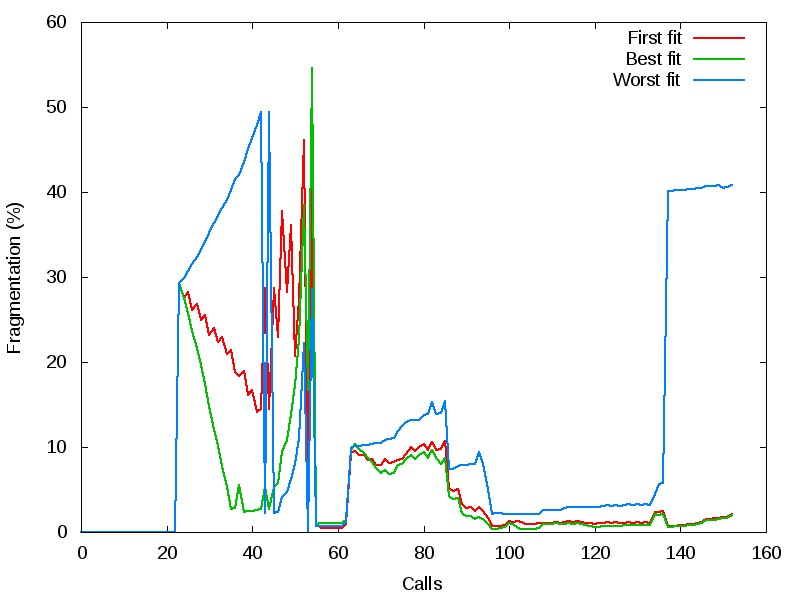
\includegraphics[width=1\linewidth]{Shashkova/images/fragment_zip.jpg}}
   \caption{Величина фрагментации с мутатором zip}
   \label{ris:image}
   \end{figure}
   
   Можно заметить, что первом участке у всех трех аллокаторов величина фрагментации равна 0. Это связано с тем, что освобождения памяти еще не производились и объекты
   находятся в куче последовательно, без пропусков. Затем фрагментация начинает возрастать. Как и предполагалось теоретически, почти на всех участках графика 
   фрагментация аллокатора Worst fit больше фрагментации остальных аллокаторов, а фрагментация аллокатора Best fit меньше фрагментации остальных аллокаторов.
   
   \begin{figure}[p]
   \center{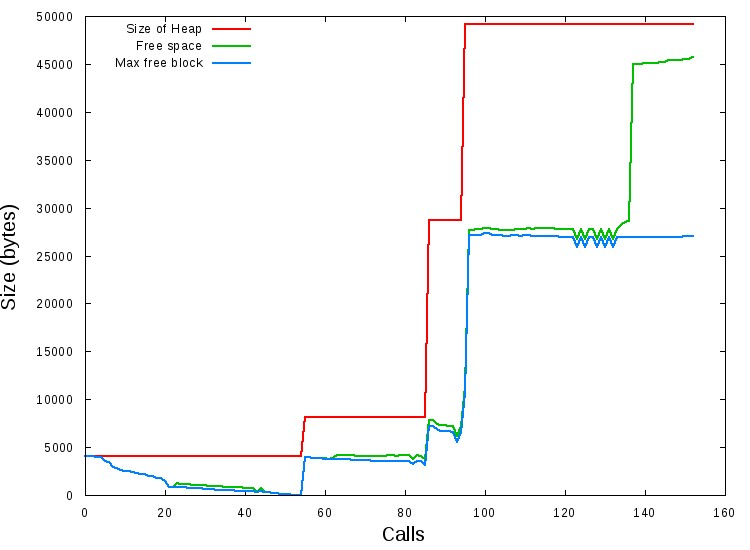
\includegraphics[width=1\linewidth]{Shashkova/images/size_zip_worst.jpg}}
   \caption{Состояние кучи с аллокаторм Worst fit и мутатором zip}
   \label{ris:image}
   \end{figure}
   
   Можно отметить резкий скачок, а затем резкое уменьшение фрагментации в районе 60-го запроса. Для объяснения такого поведения, рассмотрим график размера кучи, 
   например, для аллокатора Worst fit(см. Рис. 2). На нем представлены размер кучи, размер свободного пространства в куче и величина максимального свободного
   блока.
   Тогда становится понятным, что резкое изменение фрагментации в районе 60-го запроса связано с увеличением размера кучи (добавляется большой свободный блок). 
   Подобное повторяется в районе 82-го и 98-го запросов, однако, там фрагментация изменяется не столь резко. Это связано с тем, что общий размер кучи к тому моменту
   уже значительно увеличился.
   
   
   \begin{figure}[p]
   \center{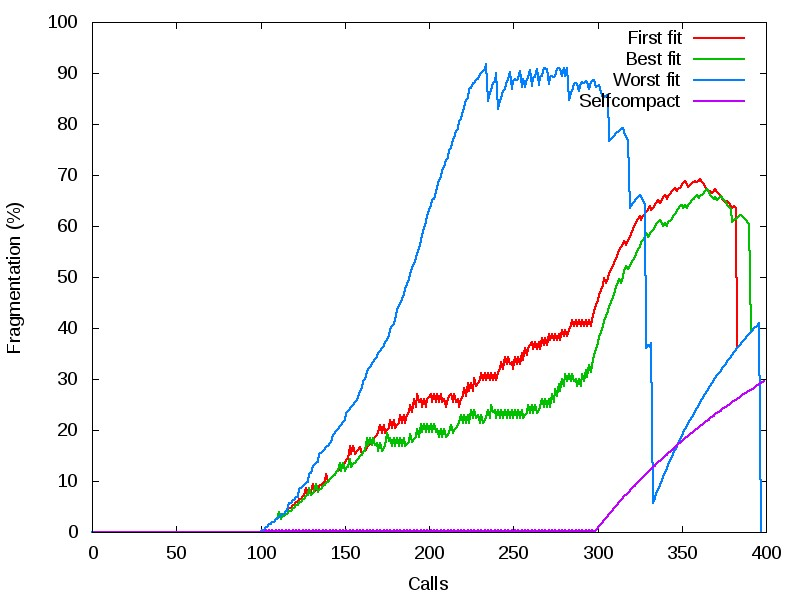
\includegraphics[width=1\linewidth]{Shashkova/images/fragment_list_selfcomp.jpg}}
   \caption{Величина фрагментации с мутатором sort list}
   \label{ris:image}
   \end{figure}
   
   На Рис. 3 представлена величина фрагментации в процессе исполнения программы --- сортировки связного списка --- для четырех аллокаторов. На первом участке графика
   видно, что для всех аллокатором величина фрагментации равна 0. На этом участке список создается, объекты располагаются в куче последовательно и все свободное
   пространство является одним блоком. 
   
   Затем, в процессе сортировки, некоторые объекты удаляются, под новые выделяется память. Здесь сразу можно заметить, что фрагментация алгоритма Worst fit растет
   быстрее фрагментации других алгоритмов. Около 300-го запроса можно отметить увеличение фрагментации у алгоритмов First fit и Best fit. 
   
   \begin{figure}[p]
   \center{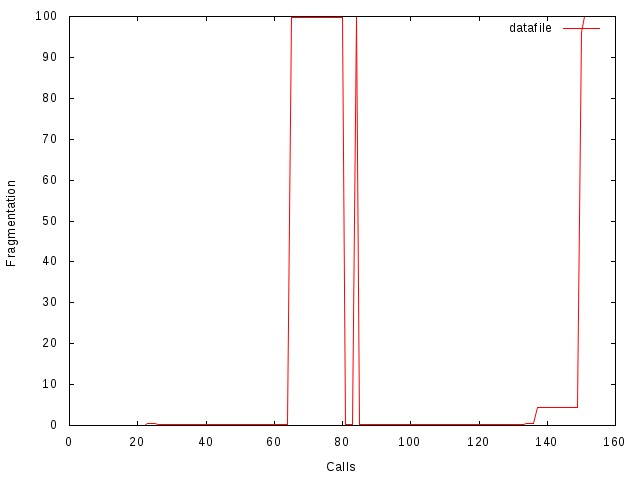
\includegraphics[width=1\linewidth]{Shashkova/images/fragment_bad.jpg}}
   \caption{Величина фрагментации аллокатора First fit}
   \label{ris:image}
   \end{figure}
   
    Хочется отметить, что сбор статистики помог выявить ошибку в первоначальной реализации аллокатора First fit. На Рис. 4 представлено, как изменялась фрагментация
   на одной из первых тестовых программ. 
   Такое резкое изменение фрагментации показалось нам неестественным. Благодаря этому была проведена перепроверка реализации и 
   выявлена ошибка.
   
   \begin{figure}[p]
   \center{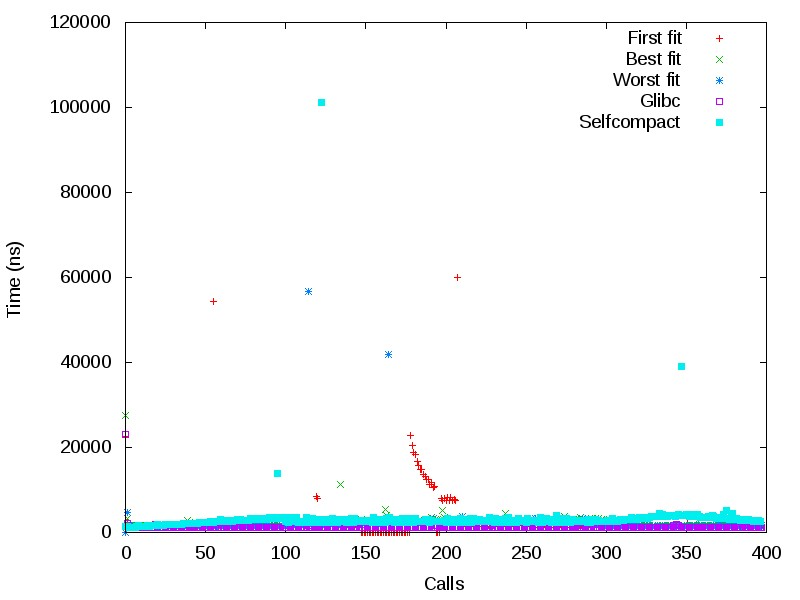
\includegraphics[width=1\linewidth]{Shashkova/images/time_gettime.jpg}}
   \caption{Время выполнения запросов}
   \label{ris:image}
   \end{figure}
   
   Также для различных алгоритмов измерялось время, затраченное аллокаторами на выполнение запросов. На Рис. 5 представлены результаты измерения времени в процессе
   работы программы. Можно заметить, что при некоторых запросах, время в несколько раз превышает среднее время на выделение. Это происходит на запросах о 
   выделении памяти, и, вероятно, это связано с поиском подходящего свободного блока. 
   
   \begin{figure}[p]
   \center{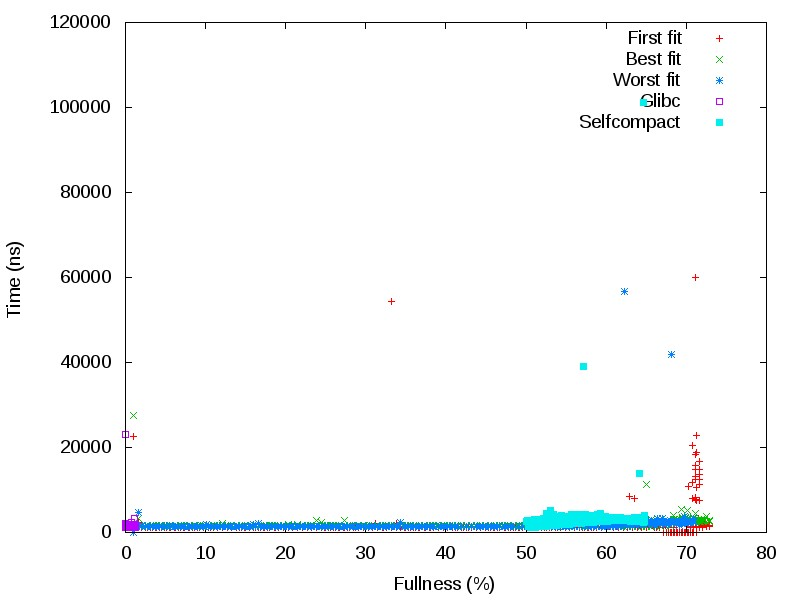
\includegraphics[width=1\linewidth]{Shashkova/images/time_full_self.jpg}}
   \caption{Зависимость времени выполнения запросов от заполненности кучи}
   \label{ris:image}
   \end{figure}
   
   \begin{figure}[p]
   \center{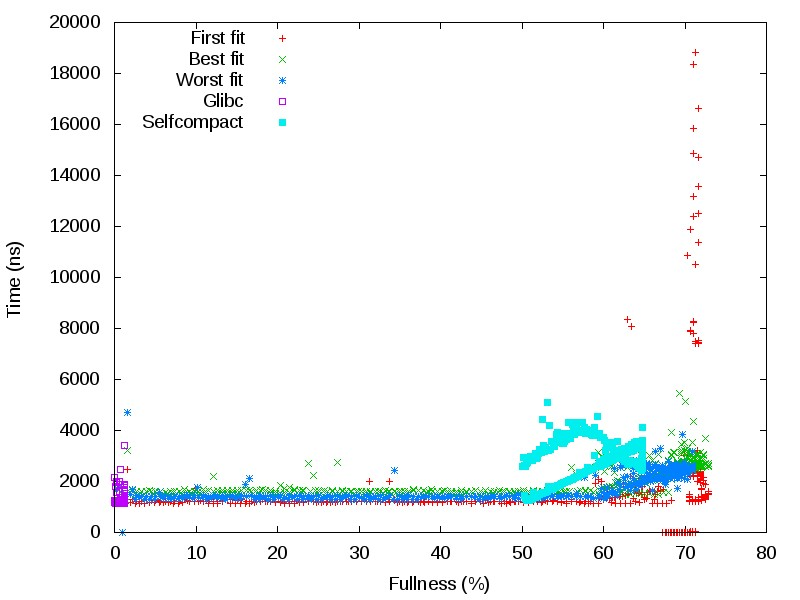
\includegraphics[width=1\linewidth]{Shashkova/images/time_full_zoom_3.jpg}}
   \caption{Зависимость времени выполнения запросов от заполненности кучи, увеличенный масштаб}
   \label{ris:image}
   \end{figure}
   
   На Рис. 6 представлена зависимость времени выделения от заполненности кучи. Наиболее выражена эта зависимость для алгоритма First fit. На Рис. 7 изображена та же
   зависимость с увеличенным масштабом для нижней части графика. На нём видно, что время выполнения запросов у самосжимающейся кучи больше, чем у остальных 
   алгоритмов. Также у всех алгоритмов наблюдается увеличение времени выполнения запросов с приближением заполненности кучи к наибольшему значению.
   
   
   \section{Заключение}
   
   В результате работы над данной курсовой работой:
   
    \begin{itemize}
     \item были изучены существующие метрики для сравнения реализаций кучи;
     \item были изучены подходы для проведения измерений;
     \item была создана система сравнения различных реализаций;
     \item была выявлена ошибка в реализации кучи.
    \end{itemize}

\begin{thebibliography}{99}
\bibitem{six_progs}
Benjamin Zorn, Dirk Grunwald.
Empirical Measurements of Six Allocation-intensive C Programs. University of Colorado, Boulder, 1992.

\bibitem{fragm}
Mark S. Johnstone, Paul R. Wilson.
The Memory Fragmentation Problem: Solved? The University of Texas at Austin, 1997.

\bibitem{un_mutator}
Martin Aigner, Christoph M. Kirsch. Towards a Universal Mutator for Benchmarking Heap Management Systems.
University of Salzburg, 2012.

\bibitem{ae}
James R. Larus. Abstract Execution: a Technique for Efficiently Tracing Programs.
Software --- Practice and Experience.

\bibitem{samofal}
Самофалов А.В. Способы реализации кучи и их свойства // Наст. сборник
\end{thebibliography}

%\documentclass[12pt,a4paper]{article}
%\usepackage[utf8x]{inputenc}
%\usepackage[russian]{babel}
%\usepackage[OT1]{fontenc}
%\usepackage{amsmath}
%\usepackage[a4paper,includeheadfoot,top=20mm,bottom=20mm,left=25mm,right=15mm]{geometry}
%\usepackage{indentfirst}
%\usepackage{amsfonts}
%\usepackage{amssymb}
%\usepackage{graphicx}
%\renewcommand\baselinestretch{1.5}
%\renewcommand\contentsname{Оглавление}

%\begin{document}
%\begin{titlepage}
%\thispagestyle{empty}
%\def\baselinestretch{1.0}
%\begin{center}
%	{\large САНКТ-ПЕТЕРБУРГСКИЙ ГОСУДАРСТВЕННЫЙ УНИВЕРСИТЕТ \\ \vskip 0.3em {\large Математико-механический факультет \\ \vskip 0.7em{\large Кафедра системного программирования \\}}}
%    \vspace*{0.15\textheight}
%    \vfill
%    {\large Шашкова Елизавета Михайловна}
%    
%    \vskip 2em
%    {\huge Методы профилирования реализаций кучи}
%    
%    \vskip 1em
%    {\large Курсовая работа} \\
%    \vskip 2em
%    {\normalsize \raggedleft 
%    Научный руководитель:\\
%    к.ф.-м.н. Д.Ю. Булычев
%    \\[3em]
%    \vspace*{0.08\textheight}
%    \vfill
%    {\centering Санкт-Петербург \\ 2013}
%    }
%\end{center}
%\end{titlepage}

\title{Методы профилирования реализаций кучи}
%
\titlerunning{Методы профилирования реализаций кучи}
\author{Шашкова Елизавета Михайловна}
%
\authorrunning{Е.М.Шашкова} % abbreviated author list (for running head)
%
%%%% list of authors for the TOC (use if author list has to be modified)
\tocauthor{Е.М.Шашкова}
%
\institute{Санк-Петербургский государственный университет\\
\email{Elizaveta239@yandex.ru}}

\maketitle              % typeset the title of the contribution

\begin{abstract}
\end{abstract}
%

\section*{Введение}

   Динамическое управление памятью --- это управление памятью для объектов, ни размер, ни время жизни которых, вообще говоря, неизвестны до
   выполнения программы. Под объектом мы будем понимать некоторый неделимый набор байт.
   
   Обычно при динамическом управлении памятью место под объекты выделяется в специальной области памяти --- \textquotedblleft куче\textquotedblright
   (heap). Существует
   две основных операции для управления памятью в куче: выделение памяти и освобождение. При выделении посылается запрос, в котором указывается количество
   требуемой памяти. При успешном выделении память изымается из кучи, то есть становится недоступна для последующего выделения.
   Освобождение памяти, наоборот, делает часть кучи доступной для последующего выделения.
   
   Поведение динамической памяти удобно описывать в терминах взаимодействия двух основных сущностей: \emph{аллокатора} и \emph{мутатора}. Аллокатор принимает запросы на выделение
   памяти в куче и её освобождение. Мутатор посылает данные запросы. Каждый запрос содержит количество памяти для выделения, причем 
   это количество, вообще говоря, становится известно только в момент исполнения программы.
   
   Эффективность работы программы во многом зависит от эффективности аллокатора. На сегодняшний момент существует много способов его 
   реализации; более того, развитие технологий стимулирует создание новых подходов. Поэтому становится важной задача уметь сравнивать разные
   реализации аллокаторов, находить наиболее подходящие реализации в данном конкретном случае.
   
   Для описания свойств аллокатора можно выделить два полярных подхода:
   \begin{enumerate}
   \item Рассмотрение свойств кучи с точки зрения поведения мутатора. Задача: определить, для какого класса программ данная реализация аллокатора 
   подойдет лучше всего. 
   \item Сравнительный анализ нескольких реализаций аллокатора. Задача: провести сравнение двух или нескольких аллокаторов при взаимодействии с
   одним и тем же мутатором.
   \end{enumerate}
   
   Основные свойства, которыми можно описать аллокатор в первом подходе:
   \begin{itemize}
   \item Суммарное количество выделенной памяти (в байтах и блоках).
   \item Наибольшее количество единовременно выделенной памяти за все время работы программы (в байтах и блоках).
   \item Среднее время жизни блока (в байтах). Это время вычисляется, как количество байт, помещенных в кучу за промежуток времени между 
   созданием и удалением объекта, поделенное на размер объекта (среднее время жизни одного байта в куче).
   \end{itemize}
   
   Основные свойства, которыми можно описать аллокатор во втором подходе:
   \begin{itemize}
   \item Фрагментация. Фрагментация вычисляется по следующей формуле: \[ F = \frac{free - free_{max}}{free} \]
   где $free$ --- количество свободных байт в куче, $free_{max}$ --- размер (в байтах) наибольшего свободного блока.  Так как память в куче выделяется
   блоками (наборами байтов), может так случиться, что в куче не осталось места для блока требуемого размера, хотя количество свободной 
   памяти еще превышает размер этого блока. С помощью данной формулы фрагментацию можно описать численной величиной. Чем меньше эта
   величина, тем \textquotedblleft лучше\textquotedblright~текущее состояние кучи. Фрагментации равна нулю, когда свободное место в 
   куче является одним блоком, и приближается к единице, когда размеры всех свободных блоков в куче малы. 
   \item Время выделения (в единицах времени).
   \item Порог работоспособности (количество запросов, обработанных аллокатором).
   \item Зависимость скорости работы аллокатора от нагрузки.
   \end{itemize}
    
   Цель данной курсовой работы заключается в том, чтобы изучить методы оценки реализации аллокатора. Необходимо понять, насколько 
   эффективно использование того или иного аллокатора, определить критерии, по которым различные аллокаторы будут сравниваться. В 
   соответствии с основными подходами, нужно сравнить поведение одного аллокатора при использовании нескольких различных мутаторов, а также
   сравнить поведение нескольких аллокаторов при работе с одним мутатором. В результате будет создан прототип системы для проведения 
   вышеуказанных сравнений.
   
   
   \section{Существующие подходы и метрики}
   Для сравнения различных реализаций аллокаторов прежде всего нужно выбрать метрики, по которым будет 
   производиться сравнение. Требуется понять, какие данные нужно собирать при запуске программ
   с использованием различных аллокаторов.
   
   В статье ~\cite{six_progs} представлены опытные данные, полученные с помощью шести программ на языке
   C. Авторы запустили каждую программу на нескольких наборах входных данных и построили распределения для следующих величин:
   
   \begin{itemize}
   \item размеров объектов;
   \item времён жизни объектов;
   \item интервалов времени между запросами.
   \end{itemize}
   
   Для этих распределений были найдены среднее, медиана и мода, которые характеризуют асимметричность распределения. Распределение размеров 
   объектов оказалось асимметричным 
   в сторону маленьких размеров: большая часть объектов, под которые выделялась память, имели размер менее 64 байт. Интересным
   оказался тот факт, что 90\% объектов имеют всего 10 различных размеров. Распределение времени жизни
   объектов показало, что большинство объектов живет в течение короткого промежутка времени: 40-80 машинных инструкций процессора 
   
   Данные об использовании памяти были получены посредством трассировки с помощью методики abstract execution~\cite{ae}. В качестве 
   тестовых программ для измерения были взяты: программа, находящая факториал больших целых чисел; оптимизатор Espresso; 
   GhostScript\footnote{http://www.ghostscript.com/} –-- интерпретатор языка PostScript; Gnu Awk\footnote{http://www.gnu.org/software/gawk/} –-- 
   интерпретатор языка AWK; интерпретатор Perl\footnote{http://www.perl.org/}; Chameleon –-- канальный роутер N-го уровня.
   
   Такой способ анализа аллокаторов нельзя полностью отнести ни к первому, ни ко второму подходу, т.к. в программах аллокатор и мутатор
   были фиксированными, изменялись только входные данные. Приоритетом для авторов являлось исследование свойств объектов, для которых выделяется
   память, а не аллокаторов.
   
   В статье ~\cite{fragm} авторы анализировали выделение памяти в нескольких приложениях, чтобы показать, что фрагментацию
   во время исполнения программы можно уменьшить посредством правильного выбора аллокатора. Было показано, что объекты,
   которые помещаются в кучу одновременно, удаляются из неё также одновременно. 
   Параметры, измерявшиеся в процессе работы программ, были таковы:
   
   \begin{itemize}
      \item время работы;
      \item суммарное количество выделенных объектов и байт;
      \item средний размер объектов;
      \item наибольшее количество объектов и байт, одновременно находящихся в куче;
      \item среднее время жизни объектов (в байтах).
   \end{itemize}
   
   Также, как и в предыдущей статье, было показано, что динамические объекты имеют обычно несколько определенных размеров. Был сделан
   вывод, что для уменьшения фрагментации при создании системы выделения памяти нужно опираться прежде всего на данное свойство программ.
   
   В данном исследовании авторы использовали как первый, так и второй подход. Они измеряли фрагментацию по всевозможным комбинациям имеющихся 
   у них мутаторов и аллокаторов.
   
   В ~\cite{un_mutator} авторы описывают созданный ими универсальный мутатор --- ACDC Benchmark Tool. Он представляет собой измеритель, 
   который может эмулировать выделение и очистку памяти и показывать различия между реализациями аллокаторов. Основная идея, заложенная в данном 
   измерителе, заключается в том, чтобы рассматривать в качестве метрики время и измерять его в байтах. Это было сделано для работы не только с
   однопоточными, но и с многопоточными мутаторами. 
   
   С помощью данного инструмента можно осуществить измерения в рамках как первого, так и второго подхода.
   
   
   \section{Проведение измерений}
   В данной работе были реализованы оба подхода к сбору данных. Для первого подхода, который заключается в рассмотрении свойств аллокатора с точки зрения мутатора, измерялись следующие величины:
   \begin{itemize}
      \item суммарное количество выделенной памяти (в байтах и блоках);
      \item наибольшее количество единовременно выделенной памяти за все время работы программы (в байтах и блоках);
      \item среднее время жизни блока (в байтах).
   \end{itemize}
      
   Для второго подхода, основная цель которого --- сравнить аллокаторы с использованием одного мутатора, 
   измерялись:
   \begin{itemize}
         \item фрагментация; 
         \item время выделения (в единицах времени);
         \item порог работоспособности (количество запросов, обработанных аллокатором);
         \item зависимость скорости работы аллокатора от нагрузки.
   \end{itemize}
      
   \subsection{Аллокаторы и мутаторы}
   
   Сбор данных производился как со стандартной реализации аллокатора в glibc, так и с собственной реализации,
   созданной Самофаловым А.В. ~\cite{samofal}. В его работе было реализовано несколько аллокаторов с различными алгоритмами
   выделения памяти.
   
   Эти алгоритмы:
   \begin{itemize}
      \item \textquotedblleft First fit\textquotedblright --- память выделяется в первом свободном блоке;
      \item \textquotedblleft Best fit\textquotedblright --- память выделяется в наиболее подходящем блоке;
      \item \textquotedblleft Worst fit\textquotedblright --- память выделяется в самом большом свободном блоке;
      \item \textquotedblleft Selfcompact\textquotedblright --- cамосжимающаяся куча.
   \end{itemize}
   
   В качестве мутаторов были взяты следующие программы:
   \begin{itemize}
        \item архиватор zip\footnote{http://www.info-zip.org};
   	    \item программа, сортирующая связный список --- sort list;
   	    \item архиватор tar\footnote{http://www.gnu.org/software/tar/}.
   \end{itemize}
   
   \subsection{Подробности реализации}
   
   В стандартной библиотеке языка C существует специальная структура \texttt{mallinfo}, которая описывает состояние кучи. Данная структура имеет следующие поля: 
   \begin{itemize}
   	     \item \texttt{int arena} --- суммарное пространство, выделенное под кучу (в байтах).
         \item \texttt{int ordblks} --- количество свободных блоков.
         \item \texttt{int smblks} --- количество свободных блоков \textquotedblleft fastbin\textquotedblright. Это блоки, которые были освобождены,
         однако, не были объединены с соседними свободными блоками. В этих блоках впоследствии можно 
         выделять память под объекты такого же размера.
          \item \texttt{int hblks} --- суммарное количество блоков, находящихся в куче.
          \item \texttt{int hblkhd} --- суммарное место, выделенное под блоки (в байтах).
          \item \texttt{int usmblks} --- наибольшее количество байт, находящихся в куче за время работы программы.
          \item \texttt{int fsmblks} --- суммарное место в блоках \textquotedblleft fastbin\textquotedblright (в байтах).
          \item \texttt{int uordblks} --- суммарное занятое пространство (в байтах).
          \item \texttt{int fordblks} --- суммарное свободное пространство (в байтах).
          \item \texttt{int keepcost} --- наибольшее количество пространства, которое можно освободить в начале кучи 
          (то есть посредством функции \texttt{malloc\_trim}) (в байтах).
   \end{itemize}
   
   Функция \texttt{mallinfo} возвращает копию структуры \texttt{mallinfo}. С её помощью были измерены некоторые величины для стандартной реализации аллокатора. 
   Для осуществления измерений были использованы hook-функции. Переменные \texttt{\_\_malloc\_hook}, \texttt{\_\_realloc\_hook} и \texttt{\_\_free\_hook} являются 
   указателями на функции, которые используют функции \texttt{malloc}, \texttt{realloc} и \texttt{free} соответственно всякий раз, когда они вызываются. Таким 
   образом можно привязывать вызов требуемых функций (в нашем случае --- сбор статистики) к запросам на выделение или очистку памяти.
   
   В собственной реализации для сбора статистики был создан аналог структуры \texttt{mallinfo} --- структура \texttt{myinfo}.
   Её устройство схоже с устройством \texttt{mallinfo}, однако, имеются некоторые различия. Она содержит следующие поля:
   \begin{itemize}
     \item \texttt{int arena} --- суммарное пространство, выделенное под кучу (в байтах);
     \item \texttt{int freemem} --- свободное пространство (в байтах);
     \item \texttt{int usdmem} --- занятое пространство (в байтах);
     \item \texttt{int freeblks} --- количество свободных блоков;
     \item \texttt{nt usdblks} --- количество используемых блоков;
     \item \texttt{maxfreeblk} --- размер наибольшего свободного блока (в байтах).
   \end{itemize} 
   
   Основным отличием данной структуры от структуры \texttt{mallinfo} является наличие поля с размером наибольшего свободного
   блока. Оно позволяет напрямую использовать это значение для вычисления фрагментации (по формуле, упоминавшейся
   во введении).
   
   
   \section{Результаты}
   
   Результаты измерений в первом подходе --- данные, усредненные по выполнению программы. Результаты представлены в следующих таблицах. Max(bytes) обозначает
   наибольшее количество единовременно выделенной памяти(в байтах). Sum(bytes) обозначает общее количество выделенной памяти(в байтах). Mean lifetime(bytes)
   обозначает среднее время жизни блока(в байтах).
    
    First fit:
    \begin{center}
    \begin{tabular}{| l | c | c | c | c | c |}
    \hline
    Мутатор & Max(bytes) & Max(blocks) & Sum(bytes) & Sum(blocks) & Mean lifetime(bytes)\\
    \hline
    zip & 21064 & 53 & 25845 & 77 & 1068.48\\
    \hline
    sort list & 808 & 101 & 1592 & 199 & 82.21 \\
    \hline
    tar & 52080 & 238 & 58736 & 404 & 446.86 \\
    \hline
    \end{tabular}
    \end{center}

    Best fit:
    \begin{center}
    \begin{tabular}{| l | c | c | c | c | c |}
    \hline
    Мутатор & Max(bytes) & Max(blocks) & Sum(bytes) & Sum(blocks) & Mean lifetime(bytes)\\
    \hline
    zip & 21080 & 53 & 25845 & 75 & 1068.64\\
    \hline
    sort list & 808 & 101 & 1592 & 199 & 82.27 \\
    \hline
    tar & 52112 & 238 & 58736 & 402 & 451.89 \\
    \hline
    \end{tabular}
    \end{center}
    
    Worst fit:
    \begin{center}
    \begin{tabular}{| l | c | c | c | c | c |}
    \hline
    Мутатор & Max(bytes) & Max(blocks) & Sum(bytes) & Sum(blocks) & Mean lifetime(bytes)\\
    \hline
    zip & 21064 & 53 & 25845 & 80 & 1069.85\\
    \hline
    sort list & 808 & 101 & 1592 & 199 & 80.72\\
    \hline
    tar & 52080 & 238 & 58736 & 404 & 455.58 \\
    \hline
    \end{tabular}
    \end{center}
    
   Средние величины для всех аллокаторов получились почти одинаковые. Данный подход к изучению аллокаторов не выявил их различий и особенностей.
    
   
   Во втором подходе измерения и сравнения производились после каждого запроса, которыми обменивались между собой аллокатор и мутатор. В связи с этим,
   полученные данные удобно представить в виде графиков.
   
   На Рис. 1 представлено изменение фрагментации для алгоритмов First fit, Best fit и Worst fit при работе с программой zip. Из пяти возможных аллокаторов
   величину фрагментации с мутатором zip удалось найти только для данных трех. Это связано с тем, что для стандартной реализации аллокатора фрагментацию по нашей
   формуле найти не удастся, так как нет возможности узнать размер наибольшего свободного блока. А аллокатор selfcompact требует специфичного написания мутатора и 
   его компиляции, поэтому запустить этот аллокатор с мутатором zip не представляется возможным.
   
   \begin{figure}[h]
   \center{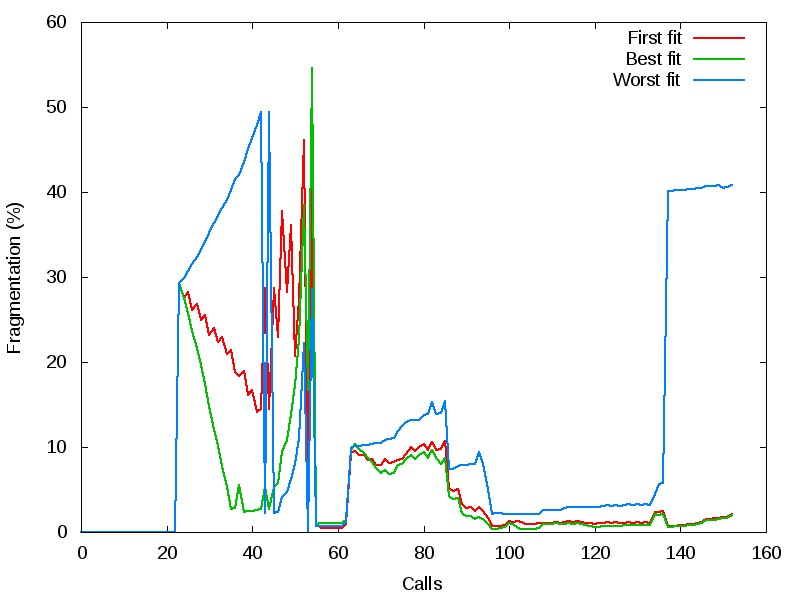
\includegraphics[width=1\linewidth]{Shashkova/images/fragment_zip.jpg}}
   \caption{Величина фрагментации с мутатором zip}
   \label{ris:image}
   \end{figure}
   
   Можно заметить, что первом участке у всех трех аллокаторов величина фрагментации равна 0. Это связано с тем, что освобождения памяти еще не производились и объекты
   находятся в куче последовательно, без пропусков. Затем фрагментация начинает возрастать. Как и предполагалось теоретически, почти на всех участках графика 
   фрагментация аллокатора Worst fit больше фрагментации остальных аллокаторов, а фрагментация аллокатора Best fit меньше фрагментации остальных аллокаторов.
   
   \begin{figure}[p]
   \center{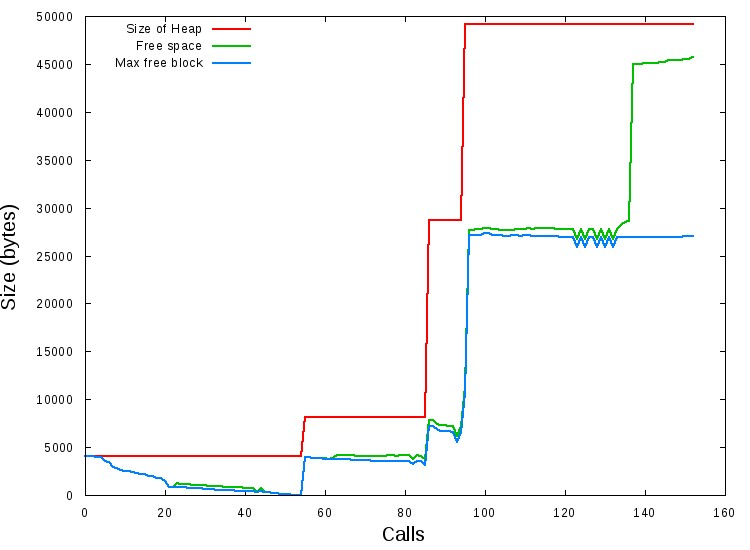
\includegraphics[width=1\linewidth]{Shashkova/images/size_zip_worst.jpg}}
   \caption{Состояние кучи с аллокаторм Worst fit и мутатором zip}
   \label{ris:image}
   \end{figure}
   
   Можно отметить резкий скачок, а затем резкое уменьшение фрагментации в районе 60-го запроса. Для объяснения такого поведения, рассмотрим график размера кучи, 
   например, для аллокатора Worst fit(см. Рис. 2). На нем представлены размер кучи, размер свободного пространства в куче и величина максимального свободного
   блока.
   Тогда становится понятным, что резкое изменение фрагментации в районе 60-го запроса связано с увеличением размера кучи (добавляется большой свободный блок). 
   Подобное повторяется в районе 82-го и 98-го запросов, однако, там фрагментация изменяется не столь резко. Это связано с тем, что общий размер кучи к тому моменту
   уже значительно увеличился.
   
   
   \begin{figure}[p]
   \center{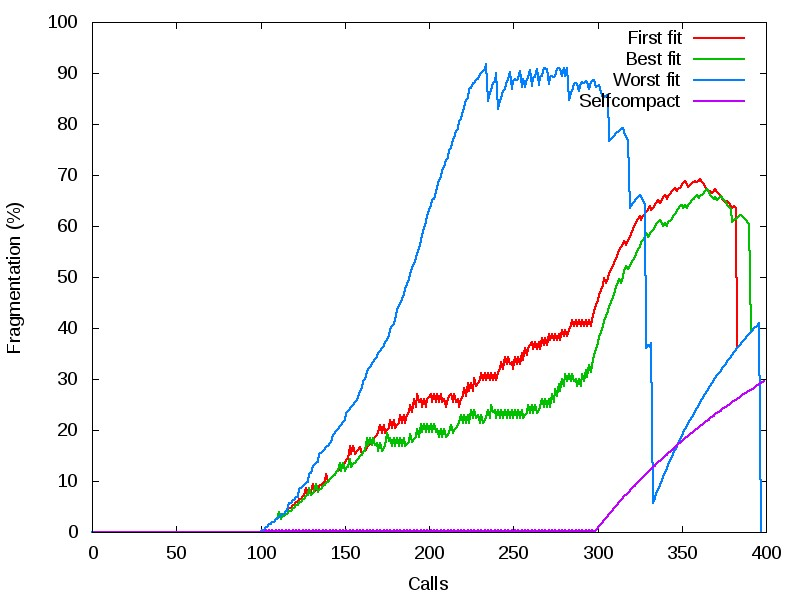
\includegraphics[width=1\linewidth]{Shashkova/images/fragment_list_selfcomp.jpg}}
   \caption{Величина фрагментации с мутатором sort list}
   \label{ris:image}
   \end{figure}
   
   На Рис. 3 представлена величина фрагментации в процессе исполнения программы --- сортировки связного списка --- для четырех аллокаторов. На первом участке графика
   видно, что для всех аллокатором величина фрагментации равна 0. На этом участке список создается, объекты располагаются в куче последовательно и все свободное
   пространство является одним блоком. 
   
   Затем, в процессе сортировки, некоторые объекты удаляются, под новые выделяется память. Здесь сразу можно заметить, что фрагментация алгоритма Worst fit растет
   быстрее фрагментации других алгоритмов. Около 300-го запроса можно отметить увеличение фрагментации у алгоритмов First fit и Best fit. 
   
   \begin{figure}[p]
   \center{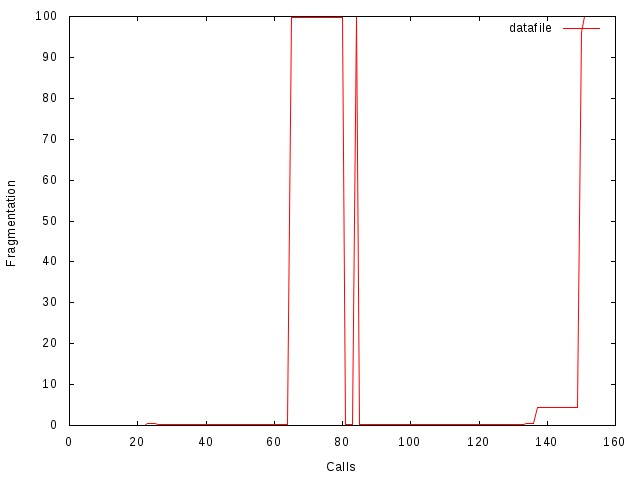
\includegraphics[width=1\linewidth]{Shashkova/images/fragment_bad.jpg}}
   \caption{Величина фрагментации аллокатора First fit}
   \label{ris:image}
   \end{figure}
   
    Хочется отметить, что сбор статистики помог выявить ошибку в первоначальной реализации аллокатора First fit. На Рис. 4 представлено, как изменялась фрагментация
   на одной из первых тестовых программ. 
   Такое резкое изменение фрагментации показалось нам неестественным. Благодаря этому была проведена перепроверка реализации и 
   выявлена ошибка.
   
   \begin{figure}[p]
   \center{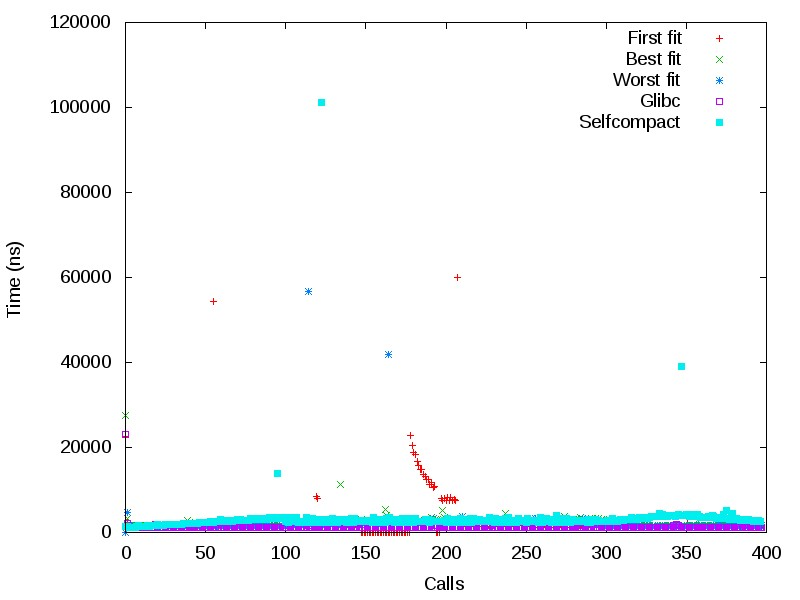
\includegraphics[width=1\linewidth]{Shashkova/images/time_gettime.jpg}}
   \caption{Время выполнения запросов}
   \label{ris:image}
   \end{figure}
   
   Также для различных алгоритмов измерялось время, затраченное аллокаторами на выполнение запросов. На Рис. 5 представлены результаты измерения времени в процессе
   работы программы. Можно заметить, что при некоторых запросах, время в несколько раз превышает среднее время на выделение. Это происходит на запросах о 
   выделении памяти, и, вероятно, это связано с поиском подходящего свободного блока. 
   
   \begin{figure}[p]
   \center{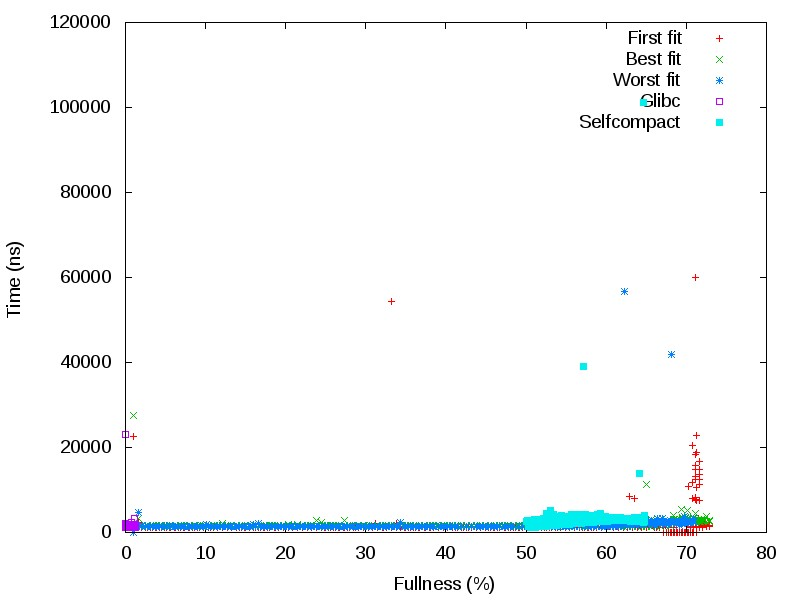
\includegraphics[width=1\linewidth]{Shashkova/images/time_full_self.jpg}}
   \caption{Зависимость времени выполнения запросов от заполненности кучи}
   \label{ris:image}
   \end{figure}
   
   \begin{figure}[p]
   \center{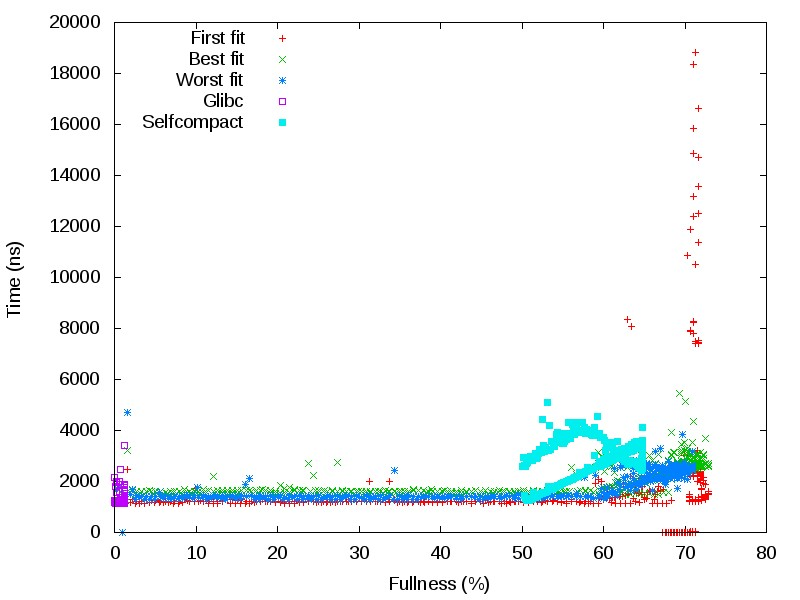
\includegraphics[width=1\linewidth]{Shashkova/images/time_full_zoom_3.jpg}}
   \caption{Зависимость времени выполнения запросов от заполненности кучи, увеличенный масштаб}
   \label{ris:image}
   \end{figure}
   
   На Рис. 6 представлена зависимость времени выделения от заполненности кучи. Наиболее выражена эта зависимость для алгоритма First fit. На Рис. 7 изображена та же
   зависимость с увеличенным масштабом для нижней части графика. На нём видно, что время выполнения запросов у самосжимающейся кучи больше, чем у остальных 
   алгоритмов. Также у всех алгоритмов наблюдается увеличение времени выполнения запросов с приближением заполненности кучи к наибольшему значению.
   
   
   \section{Заключение}
   
   В результате работы над данной курсовой работой:
   
    \begin{itemize}
     \item были изучены существующие метрики для сравнения реализаций кучи;
     \item были изучены подходы для проведения измерений;
     \item была создана система сравнения различных реализаций;
     \item была выявлена ошибка в реализации кучи.
    \end{itemize}

\begin{thebibliography}{99}
\bibitem{six_progs}
Benjamin Zorn, Dirk Grunwald.
Empirical Measurements of Six Allocation-intensive C Programs. University of Colorado, Boulder, 1992.

\bibitem{fragm}
Mark S. Johnstone, Paul R. Wilson.
The Memory Fragmentation Problem: Solved? The University of Texas at Austin, 1997.

\bibitem{un_mutator}
Martin Aigner, Christoph M. Kirsch. Towards a Universal Mutator for Benchmarking Heap Management Systems.
University of Salzburg, 2012.

\bibitem{ae}
James R. Larus. Abstract Execution: a Technique for Efficiently Tracing Programs.
Software --- Practice and Experience.

\bibitem{samofal}
Самофалов А.В. Способы реализации кучи и их свойства // Наст. сборник
\end{thebibliography}


%\documentclass[12pt,a4paper]{article}
%\usepackage[utf8x]{inputenc}
%\usepackage[russian]{babel}
%\usepackage[OT1]{fontenc}
%\usepackage{amsmath}
%\usepackage[a4paper,includeheadfoot,top=20mm,bottom=20mm,left=25mm,right=15mm]{geometry}
%\usepackage{indentfirst}
%\usepackage{amsfonts}
%\usepackage{amssymb}
%\usepackage{graphicx}
%\renewcommand\baselinestretch{1.5}
%\renewcommand\contentsname{Оглавление}

%\begin{document}
%\begin{titlepage}
%\thispagestyle{empty}
%\def\baselinestretch{1.0}
%\begin{center}
%	{\large САНКТ-ПЕТЕРБУРГСКИЙ ГОСУДАРСТВЕННЫЙ УНИВЕРСИТЕТ \\ \vskip 0.3em {\large Математико-механический факультет \\ \vskip 0.7em{\large Кафедра системного программирования \\}}}
%    \vspace*{0.15\textheight}
%    \vfill
%    {\large Шашкова Елизавета Михайловна}
%    
%    \vskip 2em
%    {\huge Методы профилирования реализаций кучи}
%    
%    \vskip 1em
%    {\large Курсовая работа} \\
%    \vskip 2em
%    {\normalsize \raggedleft 
%    Научный руководитель:\\
%    к.ф.-м.н. Д.Ю. Булычев
%    \\[3em]
%    \vspace*{0.08\textheight}
%    \vfill
%    {\centering Санкт-Петербург \\ 2013}
%    }
%\end{center}
%\end{titlepage}

\title{Методы профилирования реализаций кучи}
%
\titlerunning{Методы профилирования реализаций кучи}
\author{Шашкова Елизавета Михайловна}
%
\authorrunning{Е.М.Шашкова} % abbreviated author list (for running head)
%
%%%% list of authors for the TOC (use if author list has to be modified)
\tocauthor{Е.М.Шашкова}
%
\institute{Санк-Петербургский государственный университет\\
\email{Elizaveta239@yandex.ru}}

\maketitle              % typeset the title of the contribution

\begin{abstract}
\end{abstract}
%

\section*{Введение}

   Динамическое управление памятью --- это управление памятью для объектов, ни размер, ни время жизни которых, вообще говоря, неизвестны до
   выполнения программы. Под объектом мы будем понимать некоторый неделимый набор байт.
   
   Обычно при динамическом управлении памятью место под объекты выделяется в специальной области памяти --- \textquotedblleft куче\textquotedblright
   (heap). Существует
   две основных операции для управления памятью в куче: выделение памяти и освобождение. При выделении посылается запрос, в котором указывается количество
   требуемой памяти. При успешном выделении память изымается из кучи, то есть становится недоступна для последующего выделения.
   Освобождение памяти, наоборот, делает часть кучи доступной для последующего выделения.
   
   Поведение динамической памяти удобно описывать в терминах взаимодействия двух основных сущностей: \emph{аллокатора} и \emph{мутатора}. Аллокатор принимает запросы на выделение
   памяти в куче и её освобождение. Мутатор посылает данные запросы. Каждый запрос содержит количество памяти для выделения, причем 
   это количество, вообще говоря, становится известно только в момент исполнения программы.
   
   Эффективность работы программы во многом зависит от эффективности аллокатора. На сегодняшний момент существует много способов его 
   реализации; более того, развитие технологий стимулирует создание новых подходов. Поэтому становится важной задача уметь сравнивать разные
   реализации аллокаторов, находить наиболее подходящие реализации в данном конкретном случае.
   
   Для описания свойств аллокатора можно выделить два полярных подхода:
   \begin{enumerate}
   \item Рассмотрение свойств кучи с точки зрения поведения мутатора. Задача: определить, для какого класса программ данная реализация аллокатора 
   подойдет лучше всего. 
   \item Сравнительный анализ нескольких реализаций аллокатора. Задача: провести сравнение двух или нескольких аллокаторов при взаимодействии с
   одним и тем же мутатором.
   \end{enumerate}
   
   Основные свойства, которыми можно описать аллокатор в первом подходе:
   \begin{itemize}
   \item Суммарное количество выделенной памяти (в байтах и блоках).
   \item Наибольшее количество единовременно выделенной памяти за все время работы программы (в байтах и блоках).
   \item Среднее время жизни блока (в байтах). Это время вычисляется, как количество байт, помещенных в кучу за промежуток времени между 
   созданием и удалением объекта, поделенное на размер объекта (среднее время жизни одного байта в куче).
   \end{itemize}
   
   Основные свойства, которыми можно описать аллокатор во втором подходе:
   \begin{itemize}
   \item Фрагментация. Фрагментация вычисляется по следующей формуле: \[ F = \frac{free - free_{max}}{free} \]
   где $free$ --- количество свободных байт в куче, $free_{max}$ --- размер (в байтах) наибольшего свободного блока.  Так как память в куче выделяется
   блоками (наборами байтов), может так случиться, что в куче не осталось места для блока требуемого размера, хотя количество свободной 
   памяти еще превышает размер этого блока. С помощью данной формулы фрагментацию можно описать численной величиной. Чем меньше эта
   величина, тем \textquotedblleft лучше\textquotedblright~текущее состояние кучи. Фрагментации равна нулю, когда свободное место в 
   куче является одним блоком, и приближается к единице, когда размеры всех свободных блоков в куче малы. 
   \item Время выделения (в единицах времени).
   \item Порог работоспособности (количество запросов, обработанных аллокатором).
   \item Зависимость скорости работы аллокатора от нагрузки.
   \end{itemize}
    
   Цель данной курсовой работы заключается в том, чтобы изучить методы оценки реализации аллокатора. Необходимо понять, насколько 
   эффективно использование того или иного аллокатора, определить критерии, по которым различные аллокаторы будут сравниваться. В 
   соответствии с основными подходами, нужно сравнить поведение одного аллокатора при использовании нескольких различных мутаторов, а также
   сравнить поведение нескольких аллокаторов при работе с одним мутатором. В результате будет создан прототип системы для проведения 
   вышеуказанных сравнений.
   
   
   \section{Существующие подходы и метрики}
   Для сравнения различных реализаций аллокаторов прежде всего нужно выбрать метрики, по которым будет 
   производиться сравнение. Требуется понять, какие данные нужно собирать при запуске программ
   с использованием различных аллокаторов.
   
   В статье ~\cite{six_progs} представлены опытные данные, полученные с помощью шести программ на языке
   C. Авторы запустили каждую программу на нескольких наборах входных данных и построили распределения для следующих величин:
   
   \begin{itemize}
   \item размеров объектов;
   \item времён жизни объектов;
   \item интервалов времени между запросами.
   \end{itemize}
   
   Для этих распределений были найдены среднее, медиана и мода, которые характеризуют асимметричность распределения. Распределение размеров 
   объектов оказалось асимметричным 
   в сторону маленьких размеров: большая часть объектов, под которые выделялась память, имели размер менее 64 байт. Интересным
   оказался тот факт, что 90\% объектов имеют всего 10 различных размеров. Распределение времени жизни
   объектов показало, что большинство объектов живет в течение короткого промежутка времени: 40-80 машинных инструкций процессора 
   
   Данные об использовании памяти были получены посредством трассировки с помощью методики abstract execution~\cite{ae}. В качестве 
   тестовых программ для измерения были взяты: программа, находящая факториал больших целых чисел; оптимизатор Espresso; 
   GhostScript\footnote{http://www.ghostscript.com/} –-- интерпретатор языка PostScript; Gnu Awk\footnote{http://www.gnu.org/software/gawk/} –-- 
   интерпретатор языка AWK; интерпретатор Perl\footnote{http://www.perl.org/}; Chameleon –-- канальный роутер N-го уровня.
   
   Такой способ анализа аллокаторов нельзя полностью отнести ни к первому, ни ко второму подходу, т.к. в программах аллокатор и мутатор
   были фиксированными, изменялись только входные данные. Приоритетом для авторов являлось исследование свойств объектов, для которых выделяется
   память, а не аллокаторов.
   
   В статье ~\cite{fragm} авторы анализировали выделение памяти в нескольких приложениях, чтобы показать, что фрагментацию
   во время исполнения программы можно уменьшить посредством правильного выбора аллокатора. Было показано, что объекты,
   которые помещаются в кучу одновременно, удаляются из неё также одновременно. 
   Параметры, измерявшиеся в процессе работы программ, были таковы:
   
   \begin{itemize}
      \item время работы;
      \item суммарное количество выделенных объектов и байт;
      \item средний размер объектов;
      \item наибольшее количество объектов и байт, одновременно находящихся в куче;
      \item среднее время жизни объектов (в байтах).
   \end{itemize}
   
   Также, как и в предыдущей статье, было показано, что динамические объекты имеют обычно несколько определенных размеров. Был сделан
   вывод, что для уменьшения фрагментации при создании системы выделения памяти нужно опираться прежде всего на данное свойство программ.
   
   В данном исследовании авторы использовали как первый, так и второй подход. Они измеряли фрагментацию по всевозможным комбинациям имеющихся 
   у них мутаторов и аллокаторов.
   
   В ~\cite{un_mutator} авторы описывают созданный ими универсальный мутатор --- ACDC Benchmark Tool. Он представляет собой измеритель, 
   который может эмулировать выделение и очистку памяти и показывать различия между реализациями аллокаторов. Основная идея, заложенная в данном 
   измерителе, заключается в том, чтобы рассматривать в качестве метрики время и измерять его в байтах. Это было сделано для работы не только с
   однопоточными, но и с многопоточными мутаторами. 
   
   С помощью данного инструмента можно осуществить измерения в рамках как первого, так и второго подхода.
   
   
   \section{Проведение измерений}
   В данной работе были реализованы оба подхода к сбору данных. Для первого подхода, который заключается в рассмотрении свойств аллокатора с точки зрения мутатора, измерялись следующие величины:
   \begin{itemize}
      \item суммарное количество выделенной памяти (в байтах и блоках);
      \item наибольшее количество единовременно выделенной памяти за все время работы программы (в байтах и блоках);
      \item среднее время жизни блока (в байтах).
   \end{itemize}
      
   Для второго подхода, основная цель которого --- сравнить аллокаторы с использованием одного мутатора, 
   измерялись:
   \begin{itemize}
         \item фрагментация; 
         \item время выделения (в единицах времени);
         \item порог работоспособности (количество запросов, обработанных аллокатором);
         \item зависимость скорости работы аллокатора от нагрузки.
   \end{itemize}
      
   \subsection{Аллокаторы и мутаторы}
   
   Сбор данных производился как со стандартной реализации аллокатора в glibc, так и с собственной реализации,
   созданной Самофаловым А.В. ~\cite{samofal}. В его работе было реализовано несколько аллокаторов с различными алгоритмами
   выделения памяти.
   
   Эти алгоритмы:
   \begin{itemize}
      \item \textquotedblleft First fit\textquotedblright --- память выделяется в первом свободном блоке;
      \item \textquotedblleft Best fit\textquotedblright --- память выделяется в наиболее подходящем блоке;
      \item \textquotedblleft Worst fit\textquotedblright --- память выделяется в самом большом свободном блоке;
      \item \textquotedblleft Selfcompact\textquotedblright --- cамосжимающаяся куча.
   \end{itemize}
   
   В качестве мутаторов были взяты следующие программы:
   \begin{itemize}
        \item архиватор zip\footnote{http://www.info-zip.org};
   	    \item программа, сортирующая связный список --- sort list;
   	    \item архиватор tar\footnote{http://www.gnu.org/software/tar/}.
   \end{itemize}
   
   \subsection{Подробности реализации}
   
   В стандартной библиотеке языка C существует специальная структура \texttt{mallinfo}, которая описывает состояние кучи. Данная структура имеет следующие поля: 
   \begin{itemize}
   	     \item \texttt{int arena} --- суммарное пространство, выделенное под кучу (в байтах).
         \item \texttt{int ordblks} --- количество свободных блоков.
         \item \texttt{int smblks} --- количество свободных блоков \textquotedblleft fastbin\textquotedblright. Это блоки, которые были освобождены,
         однако, не были объединены с соседними свободными блоками. В этих блоках впоследствии можно 
         выделять память под объекты такого же размера.
          \item \texttt{int hblks} --- суммарное количество блоков, находящихся в куче.
          \item \texttt{int hblkhd} --- суммарное место, выделенное под блоки (в байтах).
          \item \texttt{int usmblks} --- наибольшее количество байт, находящихся в куче за время работы программы.
          \item \texttt{int fsmblks} --- суммарное место в блоках \textquotedblleft fastbin\textquotedblright (в байтах).
          \item \texttt{int uordblks} --- суммарное занятое пространство (в байтах).
          \item \texttt{int fordblks} --- суммарное свободное пространство (в байтах).
          \item \texttt{int keepcost} --- наибольшее количество пространства, которое можно освободить в начале кучи 
          (то есть посредством функции \texttt{malloc\_trim}) (в байтах).
   \end{itemize}
   
   Функция \texttt{mallinfo} возвращает копию структуры \texttt{mallinfo}. С её помощью были измерены некоторые величины для стандартной реализации аллокатора. 
   Для осуществления измерений были использованы hook-функции. Переменные \texttt{\_\_malloc\_hook}, \texttt{\_\_realloc\_hook} и \texttt{\_\_free\_hook} являются 
   указателями на функции, которые используют функции \texttt{malloc}, \texttt{realloc} и \texttt{free} соответственно всякий раз, когда они вызываются. Таким 
   образом можно привязывать вызов требуемых функций (в нашем случае --- сбор статистики) к запросам на выделение или очистку памяти.
   
   В собственной реализации для сбора статистики был создан аналог структуры \texttt{mallinfo} --- структура \texttt{myinfo}.
   Её устройство схоже с устройством \texttt{mallinfo}, однако, имеются некоторые различия. Она содержит следующие поля:
   \begin{itemize}
     \item \texttt{int arena} --- суммарное пространство, выделенное под кучу (в байтах);
     \item \texttt{int freemem} --- свободное пространство (в байтах);
     \item \texttt{int usdmem} --- занятое пространство (в байтах);
     \item \texttt{int freeblks} --- количество свободных блоков;
     \item \texttt{nt usdblks} --- количество используемых блоков;
     \item \texttt{maxfreeblk} --- размер наибольшего свободного блока (в байтах).
   \end{itemize} 
   
   Основным отличием данной структуры от структуры \texttt{mallinfo} является наличие поля с размером наибольшего свободного
   блока. Оно позволяет напрямую использовать это значение для вычисления фрагментации (по формуле, упоминавшейся
   во введении).
   
   
   \section{Результаты}
   
   Результаты измерений в первом подходе --- данные, усредненные по выполнению программы. Результаты представлены в следующих таблицах. Max(bytes) обозначает
   наибольшее количество единовременно выделенной памяти(в байтах). Sum(bytes) обозначает общее количество выделенной памяти(в байтах). Mean lifetime(bytes)
   обозначает среднее время жизни блока(в байтах).
    
    First fit:
    \begin{center}
    \begin{tabular}{| l | c | c | c | c | c |}
    \hline
    Мутатор & Max(bytes) & Max(blocks) & Sum(bytes) & Sum(blocks) & Mean lifetime(bytes)\\
    \hline
    zip & 21064 & 53 & 25845 & 77 & 1068.48\\
    \hline
    sort list & 808 & 101 & 1592 & 199 & 82.21 \\
    \hline
    tar & 52080 & 238 & 58736 & 404 & 446.86 \\
    \hline
    \end{tabular}
    \end{center}

    Best fit:
    \begin{center}
    \begin{tabular}{| l | c | c | c | c | c |}
    \hline
    Мутатор & Max(bytes) & Max(blocks) & Sum(bytes) & Sum(blocks) & Mean lifetime(bytes)\\
    \hline
    zip & 21080 & 53 & 25845 & 75 & 1068.64\\
    \hline
    sort list & 808 & 101 & 1592 & 199 & 82.27 \\
    \hline
    tar & 52112 & 238 & 58736 & 402 & 451.89 \\
    \hline
    \end{tabular}
    \end{center}
    
    Worst fit:
    \begin{center}
    \begin{tabular}{| l | c | c | c | c | c |}
    \hline
    Мутатор & Max(bytes) & Max(blocks) & Sum(bytes) & Sum(blocks) & Mean lifetime(bytes)\\
    \hline
    zip & 21064 & 53 & 25845 & 80 & 1069.85\\
    \hline
    sort list & 808 & 101 & 1592 & 199 & 80.72\\
    \hline
    tar & 52080 & 238 & 58736 & 404 & 455.58 \\
    \hline
    \end{tabular}
    \end{center}
    
   Средние величины для всех аллокаторов получились почти одинаковые. Данный подход к изучению аллокаторов не выявил их различий и особенностей.
    
   
   Во втором подходе измерения и сравнения производились после каждого запроса, которыми обменивались между собой аллокатор и мутатор. В связи с этим,
   полученные данные удобно представить в виде графиков.
   
   На Рис. 1 представлено изменение фрагментации для алгоритмов First fit, Best fit и Worst fit при работе с программой zip. Из пяти возможных аллокаторов
   величину фрагментации с мутатором zip удалось найти только для данных трех. Это связано с тем, что для стандартной реализации аллокатора фрагментацию по нашей
   формуле найти не удастся, так как нет возможности узнать размер наибольшего свободного блока. А аллокатор selfcompact требует специфичного написания мутатора и 
   его компиляции, поэтому запустить этот аллокатор с мутатором zip не представляется возможным.
   
   \begin{figure}[h]
   \center{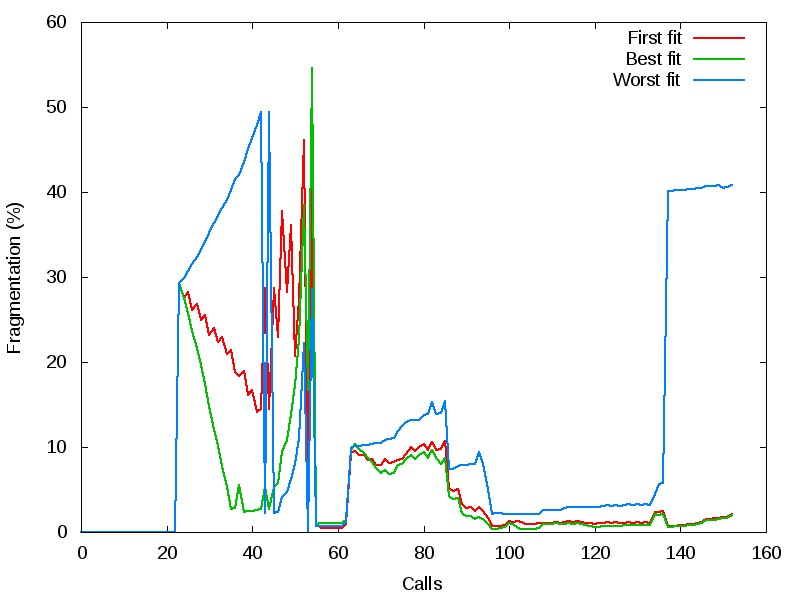
\includegraphics[width=1\linewidth]{Shashkova/images/fragment_zip.jpg}}
   \caption{Величина фрагментации с мутатором zip}
   \label{ris:image}
   \end{figure}
   
   Можно заметить, что первом участке у всех трех аллокаторов величина фрагментации равна 0. Это связано с тем, что освобождения памяти еще не производились и объекты
   находятся в куче последовательно, без пропусков. Затем фрагментация начинает возрастать. Как и предполагалось теоретически, почти на всех участках графика 
   фрагментация аллокатора Worst fit больше фрагментации остальных аллокаторов, а фрагментация аллокатора Best fit меньше фрагментации остальных аллокаторов.
   
   \begin{figure}[p]
   \center{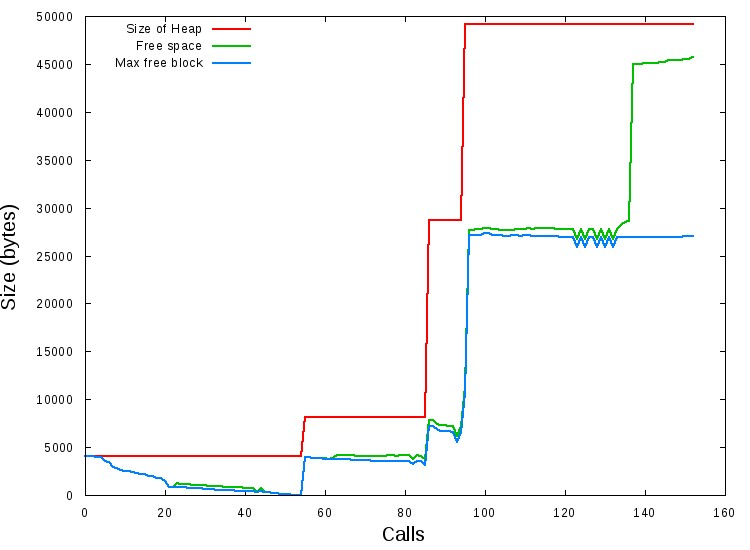
\includegraphics[width=1\linewidth]{Shashkova/images/size_zip_worst.jpg}}
   \caption{Состояние кучи с аллокаторм Worst fit и мутатором zip}
   \label{ris:image}
   \end{figure}
   
   Можно отметить резкий скачок, а затем резкое уменьшение фрагментации в районе 60-го запроса. Для объяснения такого поведения, рассмотрим график размера кучи, 
   например, для аллокатора Worst fit(см. Рис. 2). На нем представлены размер кучи, размер свободного пространства в куче и величина максимального свободного
   блока.
   Тогда становится понятным, что резкое изменение фрагментации в районе 60-го запроса связано с увеличением размера кучи (добавляется большой свободный блок). 
   Подобное повторяется в районе 82-го и 98-го запросов, однако, там фрагментация изменяется не столь резко. Это связано с тем, что общий размер кучи к тому моменту
   уже значительно увеличился.
   
   
   \begin{figure}[p]
   \center{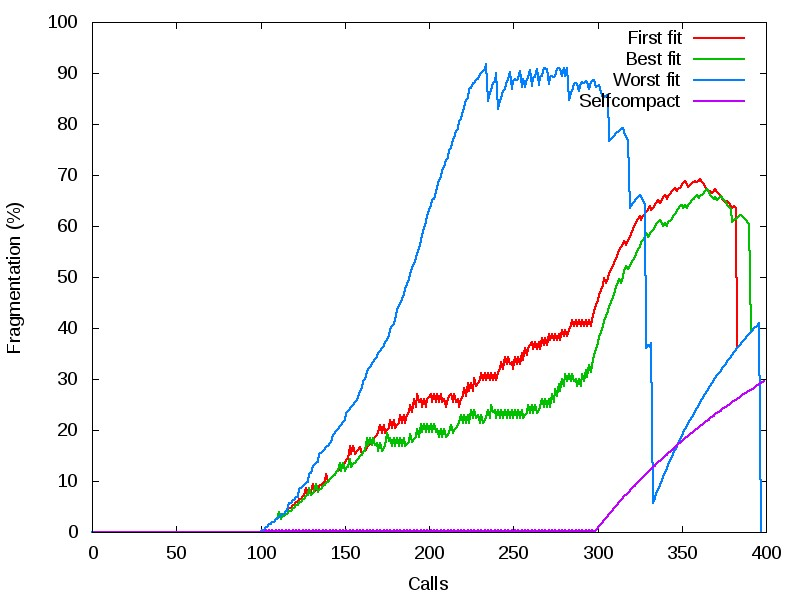
\includegraphics[width=1\linewidth]{Shashkova/images/fragment_list_selfcomp.jpg}}
   \caption{Величина фрагментации с мутатором sort list}
   \label{ris:image}
   \end{figure}
   
   На Рис. 3 представлена величина фрагментации в процессе исполнения программы --- сортировки связного списка --- для четырех аллокаторов. На первом участке графика
   видно, что для всех аллокатором величина фрагментации равна 0. На этом участке список создается, объекты располагаются в куче последовательно и все свободное
   пространство является одним блоком. 
   
   Затем, в процессе сортировки, некоторые объекты удаляются, под новые выделяется память. Здесь сразу можно заметить, что фрагментация алгоритма Worst fit растет
   быстрее фрагментации других алгоритмов. Около 300-го запроса можно отметить увеличение фрагментации у алгоритмов First fit и Best fit. 
   
   \begin{figure}[p]
   \center{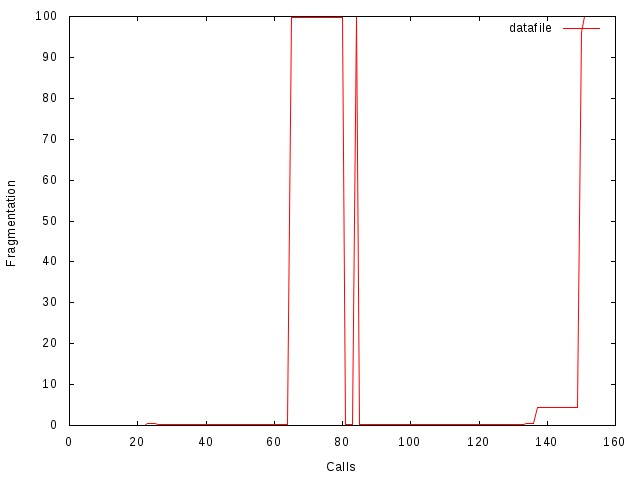
\includegraphics[width=1\linewidth]{Shashkova/images/fragment_bad.jpg}}
   \caption{Величина фрагментации аллокатора First fit}
   \label{ris:image}
   \end{figure}
   
    Хочется отметить, что сбор статистики помог выявить ошибку в первоначальной реализации аллокатора First fit. На Рис. 4 представлено, как изменялась фрагментация
   на одной из первых тестовых программ. 
   Такое резкое изменение фрагментации показалось нам неестественным. Благодаря этому была проведена перепроверка реализации и 
   выявлена ошибка.
   
   \begin{figure}[p]
   \center{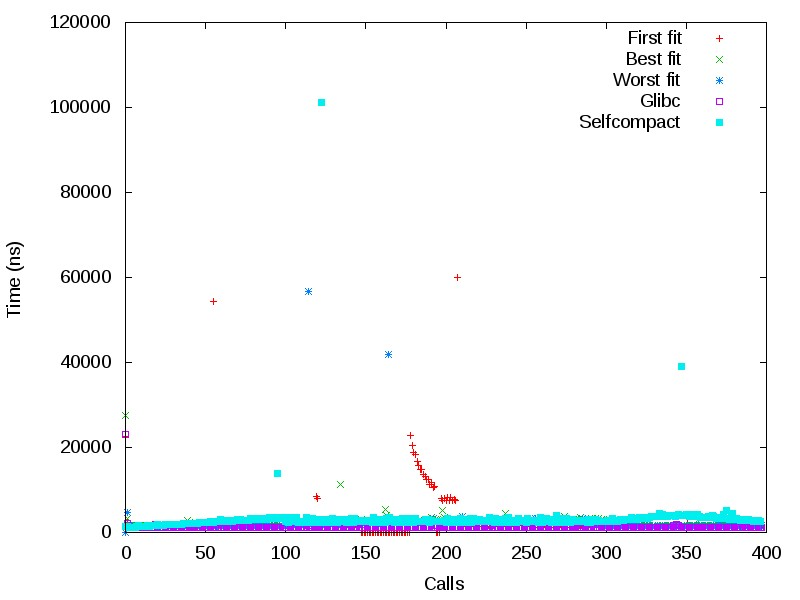
\includegraphics[width=1\linewidth]{Shashkova/images/time_gettime.jpg}}
   \caption{Время выполнения запросов}
   \label{ris:image}
   \end{figure}
   
   Также для различных алгоритмов измерялось время, затраченное аллокаторами на выполнение запросов. На Рис. 5 представлены результаты измерения времени в процессе
   работы программы. Можно заметить, что при некоторых запросах, время в несколько раз превышает среднее время на выделение. Это происходит на запросах о 
   выделении памяти, и, вероятно, это связано с поиском подходящего свободного блока. 
   
   \begin{figure}[p]
   \center{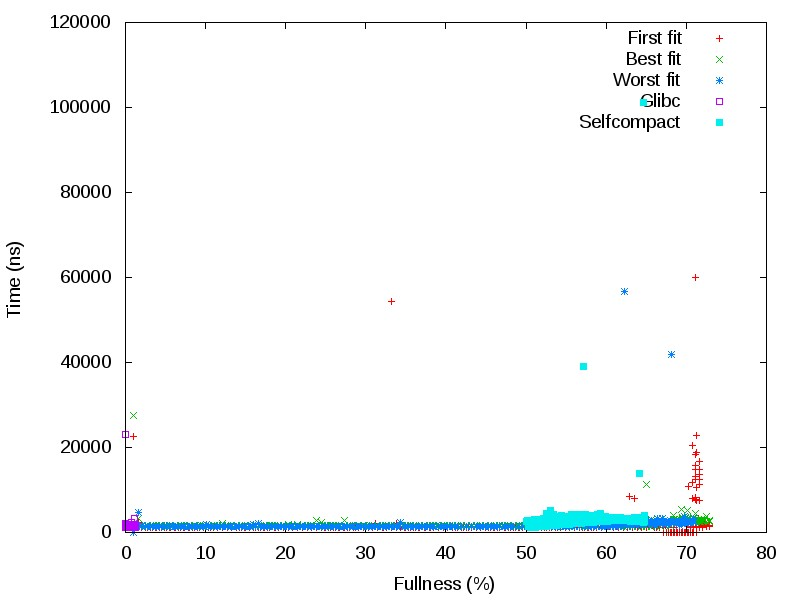
\includegraphics[width=1\linewidth]{Shashkova/images/time_full_self.jpg}}
   \caption{Зависимость времени выполнения запросов от заполненности кучи}
   \label{ris:image}
   \end{figure}
   
   \begin{figure}[p]
   \center{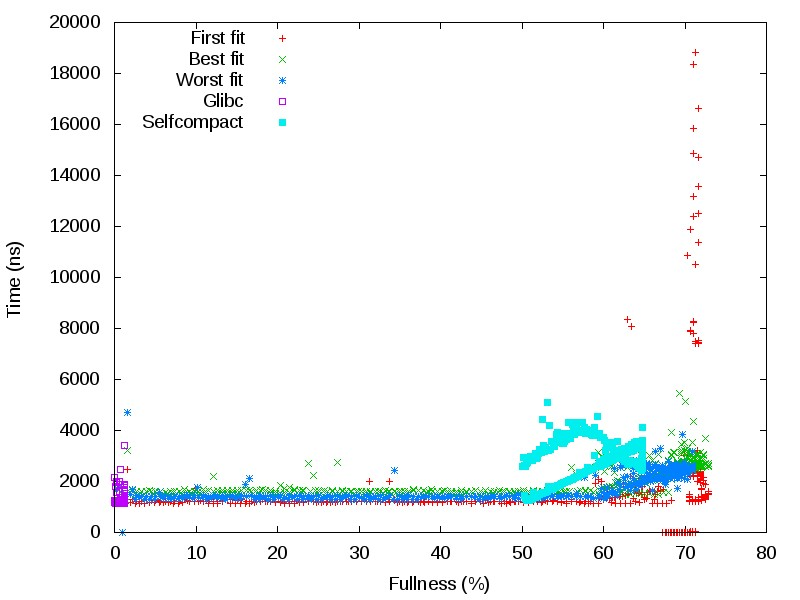
\includegraphics[width=1\linewidth]{Shashkova/images/time_full_zoom_3.jpg}}
   \caption{Зависимость времени выполнения запросов от заполненности кучи, увеличенный масштаб}
   \label{ris:image}
   \end{figure}
   
   На Рис. 6 представлена зависимость времени выделения от заполненности кучи. Наиболее выражена эта зависимость для алгоритма First fit. На Рис. 7 изображена та же
   зависимость с увеличенным масштабом для нижней части графика. На нём видно, что время выполнения запросов у самосжимающейся кучи больше, чем у остальных 
   алгоритмов. Также у всех алгоритмов наблюдается увеличение времени выполнения запросов с приближением заполненности кучи к наибольшему значению.
   
   
   \section{Заключение}
   
   В результате работы над данной курсовой работой:
   
    \begin{itemize}
     \item были изучены существующие метрики для сравнения реализаций кучи;
     \item были изучены подходы для проведения измерений;
     \item была создана система сравнения различных реализаций;
     \item была выявлена ошибка в реализации кучи.
    \end{itemize}

\begin{thebibliography}{99}
\bibitem{six_progs}
Benjamin Zorn, Dirk Grunwald.
Empirical Measurements of Six Allocation-intensive C Programs. University of Colorado, Boulder, 1992.

\bibitem{fragm}
Mark S. Johnstone, Paul R. Wilson.
The Memory Fragmentation Problem: Solved? The University of Texas at Austin, 1997.

\bibitem{un_mutator}
Martin Aigner, Christoph M. Kirsch. Towards a Universal Mutator for Benchmarking Heap Management Systems.
University of Salzburg, 2012.

\bibitem{ae}
James R. Larus. Abstract Execution: a Technique for Efficiently Tracing Programs.
Software --- Practice and Experience.

\bibitem{samofal}
Самофалов А.В. Способы реализации кучи и их свойства // Наст. сборник
\end{thebibliography}

%\documentclass[12pt,a4paper]{article}
%\usepackage[utf8x]{inputenc}
%\usepackage[russian]{babel}
%\usepackage[OT1]{fontenc}
%\usepackage{amsmath}
%\usepackage[a4paper,includeheadfoot,top=20mm,bottom=20mm,left=25mm,right=15mm]{geometry}
%\usepackage{indentfirst}
%\usepackage{amsfonts}
%\usepackage{amssymb}
%\usepackage{graphicx}
%\renewcommand\baselinestretch{1.5}
%\renewcommand\contentsname{Оглавление}

%\begin{document}
%\begin{titlepage}
%\thispagestyle{empty}
%\def\baselinestretch{1.0}
%\begin{center}
%	{\large САНКТ-ПЕТЕРБУРГСКИЙ ГОСУДАРСТВЕННЫЙ УНИВЕРСИТЕТ \\ \vskip 0.3em {\large Математико-механический факультет \\ \vskip 0.7em{\large Кафедра системного программирования \\}}}
%    \vspace*{0.15\textheight}
%    \vfill
%    {\large Шашкова Елизавета Михайловна}
%    
%    \vskip 2em
%    {\huge Методы профилирования реализаций кучи}
%    
%    \vskip 1em
%    {\large Курсовая работа} \\
%    \vskip 2em
%    {\normalsize \raggedleft 
%    Научный руководитель:\\
%    к.ф.-м.н. Д.Ю. Булычев
%    \\[3em]
%    \vspace*{0.08\textheight}
%    \vfill
%    {\centering Санкт-Петербург \\ 2013}
%    }
%\end{center}
%\end{titlepage}

\title{Методы профилирования реализаций кучи}
%
\titlerunning{Методы профилирования реализаций кучи}
\author{Шашкова Елизавета Михайловна}
%
\authorrunning{Е.М.Шашкова} % abbreviated author list (for running head)
%
%%%% list of authors for the TOC (use if author list has to be modified)
\tocauthor{Е.М.Шашкова}
%
\institute{Санк-Петербургский государственный университет\\
\email{Elizaveta239@yandex.ru}}

\maketitle              % typeset the title of the contribution

\begin{abstract}
\end{abstract}
%

\section*{Введение}

   Динамическое управление памятью --- это управление памятью для объектов, ни размер, ни время жизни которых, вообще говоря, неизвестны до
   выполнения программы. Под объектом мы будем понимать некоторый неделимый набор байт.
   
   Обычно при динамическом управлении памятью место под объекты выделяется в специальной области памяти --- \textquotedblleft куче\textquotedblright
   (heap). Существует
   две основных операции для управления памятью в куче: выделение памяти и освобождение. При выделении посылается запрос, в котором указывается количество
   требуемой памяти. При успешном выделении память изымается из кучи, то есть становится недоступна для последующего выделения.
   Освобождение памяти, наоборот, делает часть кучи доступной для последующего выделения.
   
   Поведение динамической памяти удобно описывать в терминах взаимодействия двух основных сущностей: \emph{аллокатора} и \emph{мутатора}. Аллокатор принимает запросы на выделение
   памяти в куче и её освобождение. Мутатор посылает данные запросы. Каждый запрос содержит количество памяти для выделения, причем 
   это количество, вообще говоря, становится известно только в момент исполнения программы.
   
   Эффективность работы программы во многом зависит от эффективности аллокатора. На сегодняшний момент существует много способов его 
   реализации; более того, развитие технологий стимулирует создание новых подходов. Поэтому становится важной задача уметь сравнивать разные
   реализации аллокаторов, находить наиболее подходящие реализации в данном конкретном случае.
   
   Для описания свойств аллокатора можно выделить два полярных подхода:
   \begin{enumerate}
   \item Рассмотрение свойств кучи с точки зрения поведения мутатора. Задача: определить, для какого класса программ данная реализация аллокатора 
   подойдет лучше всего. 
   \item Сравнительный анализ нескольких реализаций аллокатора. Задача: провести сравнение двух или нескольких аллокаторов при взаимодействии с
   одним и тем же мутатором.
   \end{enumerate}
   
   Основные свойства, которыми можно описать аллокатор в первом подходе:
   \begin{itemize}
   \item Суммарное количество выделенной памяти (в байтах и блоках).
   \item Наибольшее количество единовременно выделенной памяти за все время работы программы (в байтах и блоках).
   \item Среднее время жизни блока (в байтах). Это время вычисляется, как количество байт, помещенных в кучу за промежуток времени между 
   созданием и удалением объекта, поделенное на размер объекта (среднее время жизни одного байта в куче).
   \end{itemize}
   
   Основные свойства, которыми можно описать аллокатор во втором подходе:
   \begin{itemize}
   \item Фрагментация. Фрагментация вычисляется по следующей формуле: \[ F = \frac{free - free_{max}}{free} \]
   где $free$ --- количество свободных байт в куче, $free_{max}$ --- размер (в байтах) наибольшего свободного блока.  Так как память в куче выделяется
   блоками (наборами байтов), может так случиться, что в куче не осталось места для блока требуемого размера, хотя количество свободной 
   памяти еще превышает размер этого блока. С помощью данной формулы фрагментацию можно описать численной величиной. Чем меньше эта
   величина, тем \textquotedblleft лучше\textquotedblright~текущее состояние кучи. Фрагментации равна нулю, когда свободное место в 
   куче является одним блоком, и приближается к единице, когда размеры всех свободных блоков в куче малы. 
   \item Время выделения (в единицах времени).
   \item Порог работоспособности (количество запросов, обработанных аллокатором).
   \item Зависимость скорости работы аллокатора от нагрузки.
   \end{itemize}
    
   Цель данной курсовой работы заключается в том, чтобы изучить методы оценки реализации аллокатора. Необходимо понять, насколько 
   эффективно использование того или иного аллокатора, определить критерии, по которым различные аллокаторы будут сравниваться. В 
   соответствии с основными подходами, нужно сравнить поведение одного аллокатора при использовании нескольких различных мутаторов, а также
   сравнить поведение нескольких аллокаторов при работе с одним мутатором. В результате будет создан прототип системы для проведения 
   вышеуказанных сравнений.
   
   
   \section{Существующие подходы и метрики}
   Для сравнения различных реализаций аллокаторов прежде всего нужно выбрать метрики, по которым будет 
   производиться сравнение. Требуется понять, какие данные нужно собирать при запуске программ
   с использованием различных аллокаторов.
   
   В статье ~\cite{six_progs} представлены опытные данные, полученные с помощью шести программ на языке
   C. Авторы запустили каждую программу на нескольких наборах входных данных и построили распределения для следующих величин:
   
   \begin{itemize}
   \item размеров объектов;
   \item времён жизни объектов;
   \item интервалов времени между запросами.
   \end{itemize}
   
   Для этих распределений были найдены среднее, медиана и мода, которые характеризуют асимметричность распределения. Распределение размеров 
   объектов оказалось асимметричным 
   в сторону маленьких размеров: большая часть объектов, под которые выделялась память, имели размер менее 64 байт. Интересным
   оказался тот факт, что 90\% объектов имеют всего 10 различных размеров. Распределение времени жизни
   объектов показало, что большинство объектов живет в течение короткого промежутка времени: 40-80 машинных инструкций процессора 
   
   Данные об использовании памяти были получены посредством трассировки с помощью методики abstract execution~\cite{ae}. В качестве 
   тестовых программ для измерения были взяты: программа, находящая факториал больших целых чисел; оптимизатор Espresso; 
   GhostScript\footnote{http://www.ghostscript.com/} –-- интерпретатор языка PostScript; Gnu Awk\footnote{http://www.gnu.org/software/gawk/} –-- 
   интерпретатор языка AWK; интерпретатор Perl\footnote{http://www.perl.org/}; Chameleon –-- канальный роутер N-го уровня.
   
   Такой способ анализа аллокаторов нельзя полностью отнести ни к первому, ни ко второму подходу, т.к. в программах аллокатор и мутатор
   были фиксированными, изменялись только входные данные. Приоритетом для авторов являлось исследование свойств объектов, для которых выделяется
   память, а не аллокаторов.
   
   В статье ~\cite{fragm} авторы анализировали выделение памяти в нескольких приложениях, чтобы показать, что фрагментацию
   во время исполнения программы можно уменьшить посредством правильного выбора аллокатора. Было показано, что объекты,
   которые помещаются в кучу одновременно, удаляются из неё также одновременно. 
   Параметры, измерявшиеся в процессе работы программ, были таковы:
   
   \begin{itemize}
      \item время работы;
      \item суммарное количество выделенных объектов и байт;
      \item средний размер объектов;
      \item наибольшее количество объектов и байт, одновременно находящихся в куче;
      \item среднее время жизни объектов (в байтах).
   \end{itemize}
   
   Также, как и в предыдущей статье, было показано, что динамические объекты имеют обычно несколько определенных размеров. Был сделан
   вывод, что для уменьшения фрагментации при создании системы выделения памяти нужно опираться прежде всего на данное свойство программ.
   
   В данном исследовании авторы использовали как первый, так и второй подход. Они измеряли фрагментацию по всевозможным комбинациям имеющихся 
   у них мутаторов и аллокаторов.
   
   В ~\cite{un_mutator} авторы описывают созданный ими универсальный мутатор --- ACDC Benchmark Tool. Он представляет собой измеритель, 
   который может эмулировать выделение и очистку памяти и показывать различия между реализациями аллокаторов. Основная идея, заложенная в данном 
   измерителе, заключается в том, чтобы рассматривать в качестве метрики время и измерять его в байтах. Это было сделано для работы не только с
   однопоточными, но и с многопоточными мутаторами. 
   
   С помощью данного инструмента можно осуществить измерения в рамках как первого, так и второго подхода.
   
   
   \section{Проведение измерений}
   В данной работе были реализованы оба подхода к сбору данных. Для первого подхода, который заключается в рассмотрении свойств аллокатора с точки зрения мутатора, измерялись следующие величины:
   \begin{itemize}
      \item суммарное количество выделенной памяти (в байтах и блоках);
      \item наибольшее количество единовременно выделенной памяти за все время работы программы (в байтах и блоках);
      \item среднее время жизни блока (в байтах).
   \end{itemize}
      
   Для второго подхода, основная цель которого --- сравнить аллокаторы с использованием одного мутатора, 
   измерялись:
   \begin{itemize}
         \item фрагментация; 
         \item время выделения (в единицах времени);
         \item порог работоспособности (количество запросов, обработанных аллокатором);
         \item зависимость скорости работы аллокатора от нагрузки.
   \end{itemize}
      
   \subsection{Аллокаторы и мутаторы}
   
   Сбор данных производился как со стандартной реализации аллокатора в glibc, так и с собственной реализации,
   созданной Самофаловым А.В. ~\cite{samofal}. В его работе было реализовано несколько аллокаторов с различными алгоритмами
   выделения памяти.
   
   Эти алгоритмы:
   \begin{itemize}
      \item \textquotedblleft First fit\textquotedblright --- память выделяется в первом свободном блоке;
      \item \textquotedblleft Best fit\textquotedblright --- память выделяется в наиболее подходящем блоке;
      \item \textquotedblleft Worst fit\textquotedblright --- память выделяется в самом большом свободном блоке;
      \item \textquotedblleft Selfcompact\textquotedblright --- cамосжимающаяся куча.
   \end{itemize}
   
   В качестве мутаторов были взяты следующие программы:
   \begin{itemize}
        \item архиватор zip\footnote{http://www.info-zip.org};
   	    \item программа, сортирующая связный список --- sort list;
   	    \item архиватор tar\footnote{http://www.gnu.org/software/tar/}.
   \end{itemize}
   
   \subsection{Подробности реализации}
   
   В стандартной библиотеке языка C существует специальная структура \texttt{mallinfo}, которая описывает состояние кучи. Данная структура имеет следующие поля: 
   \begin{itemize}
   	     \item \texttt{int arena} --- суммарное пространство, выделенное под кучу (в байтах).
         \item \texttt{int ordblks} --- количество свободных блоков.
         \item \texttt{int smblks} --- количество свободных блоков \textquotedblleft fastbin\textquotedblright. Это блоки, которые были освобождены,
         однако, не были объединены с соседними свободными блоками. В этих блоках впоследствии можно 
         выделять память под объекты такого же размера.
          \item \texttt{int hblks} --- суммарное количество блоков, находящихся в куче.
          \item \texttt{int hblkhd} --- суммарное место, выделенное под блоки (в байтах).
          \item \texttt{int usmblks} --- наибольшее количество байт, находящихся в куче за время работы программы.
          \item \texttt{int fsmblks} --- суммарное место в блоках \textquotedblleft fastbin\textquotedblright (в байтах).
          \item \texttt{int uordblks} --- суммарное занятое пространство (в байтах).
          \item \texttt{int fordblks} --- суммарное свободное пространство (в байтах).
          \item \texttt{int keepcost} --- наибольшее количество пространства, которое можно освободить в начале кучи 
          (то есть посредством функции \texttt{malloc\_trim}) (в байтах).
   \end{itemize}
   
   Функция \texttt{mallinfo} возвращает копию структуры \texttt{mallinfo}. С её помощью были измерены некоторые величины для стандартной реализации аллокатора. 
   Для осуществления измерений были использованы hook-функции. Переменные \texttt{\_\_malloc\_hook}, \texttt{\_\_realloc\_hook} и \texttt{\_\_free\_hook} являются 
   указателями на функции, которые используют функции \texttt{malloc}, \texttt{realloc} и \texttt{free} соответственно всякий раз, когда они вызываются. Таким 
   образом можно привязывать вызов требуемых функций (в нашем случае --- сбор статистики) к запросам на выделение или очистку памяти.
   
   В собственной реализации для сбора статистики был создан аналог структуры \texttt{mallinfo} --- структура \texttt{myinfo}.
   Её устройство схоже с устройством \texttt{mallinfo}, однако, имеются некоторые различия. Она содержит следующие поля:
   \begin{itemize}
     \item \texttt{int arena} --- суммарное пространство, выделенное под кучу (в байтах);
     \item \texttt{int freemem} --- свободное пространство (в байтах);
     \item \texttt{int usdmem} --- занятое пространство (в байтах);
     \item \texttt{int freeblks} --- количество свободных блоков;
     \item \texttt{nt usdblks} --- количество используемых блоков;
     \item \texttt{maxfreeblk} --- размер наибольшего свободного блока (в байтах).
   \end{itemize} 
   
   Основным отличием данной структуры от структуры \texttt{mallinfo} является наличие поля с размером наибольшего свободного
   блока. Оно позволяет напрямую использовать это значение для вычисления фрагментации (по формуле, упоминавшейся
   во введении).
   
   
   \section{Результаты}
   
   Результаты измерений в первом подходе --- данные, усредненные по выполнению программы. Результаты представлены в следующих таблицах. Max(bytes) обозначает
   наибольшее количество единовременно выделенной памяти(в байтах). Sum(bytes) обозначает общее количество выделенной памяти(в байтах). Mean lifetime(bytes)
   обозначает среднее время жизни блока(в байтах).
    
    First fit:
    \begin{center}
    \begin{tabular}{| l | c | c | c | c | c |}
    \hline
    Мутатор & Max(bytes) & Max(blocks) & Sum(bytes) & Sum(blocks) & Mean lifetime(bytes)\\
    \hline
    zip & 21064 & 53 & 25845 & 77 & 1068.48\\
    \hline
    sort list & 808 & 101 & 1592 & 199 & 82.21 \\
    \hline
    tar & 52080 & 238 & 58736 & 404 & 446.86 \\
    \hline
    \end{tabular}
    \end{center}

    Best fit:
    \begin{center}
    \begin{tabular}{| l | c | c | c | c | c |}
    \hline
    Мутатор & Max(bytes) & Max(blocks) & Sum(bytes) & Sum(blocks) & Mean lifetime(bytes)\\
    \hline
    zip & 21080 & 53 & 25845 & 75 & 1068.64\\
    \hline
    sort list & 808 & 101 & 1592 & 199 & 82.27 \\
    \hline
    tar & 52112 & 238 & 58736 & 402 & 451.89 \\
    \hline
    \end{tabular}
    \end{center}
    
    Worst fit:
    \begin{center}
    \begin{tabular}{| l | c | c | c | c | c |}
    \hline
    Мутатор & Max(bytes) & Max(blocks) & Sum(bytes) & Sum(blocks) & Mean lifetime(bytes)\\
    \hline
    zip & 21064 & 53 & 25845 & 80 & 1069.85\\
    \hline
    sort list & 808 & 101 & 1592 & 199 & 80.72\\
    \hline
    tar & 52080 & 238 & 58736 & 404 & 455.58 \\
    \hline
    \end{tabular}
    \end{center}
    
   Средние величины для всех аллокаторов получились почти одинаковые. Данный подход к изучению аллокаторов не выявил их различий и особенностей.
    
   
   Во втором подходе измерения и сравнения производились после каждого запроса, которыми обменивались между собой аллокатор и мутатор. В связи с этим,
   полученные данные удобно представить в виде графиков.
   
   На Рис. 1 представлено изменение фрагментации для алгоритмов First fit, Best fit и Worst fit при работе с программой zip. Из пяти возможных аллокаторов
   величину фрагментации с мутатором zip удалось найти только для данных трех. Это связано с тем, что для стандартной реализации аллокатора фрагментацию по нашей
   формуле найти не удастся, так как нет возможности узнать размер наибольшего свободного блока. А аллокатор selfcompact требует специфичного написания мутатора и 
   его компиляции, поэтому запустить этот аллокатор с мутатором zip не представляется возможным.
   
   \begin{figure}[h]
   \center{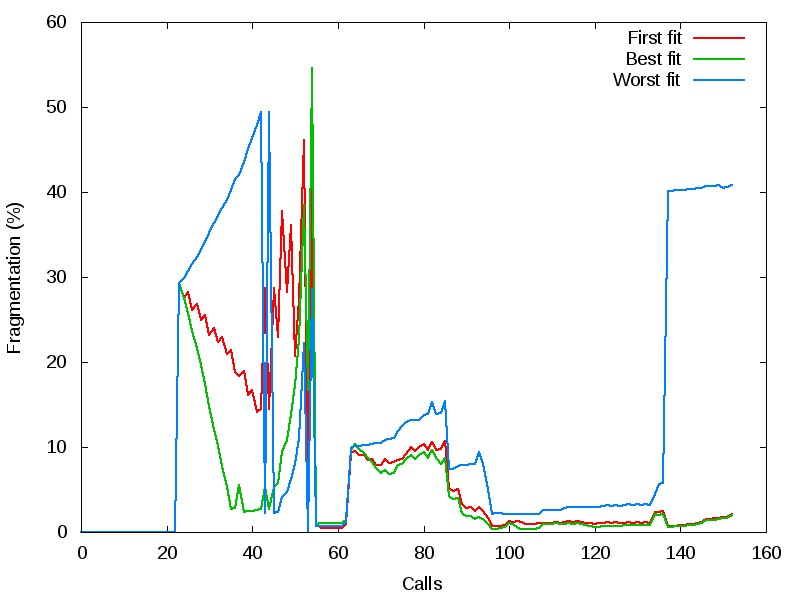
\includegraphics[width=1\linewidth]{Shashkova/images/fragment_zip.jpg}}
   \caption{Величина фрагментации с мутатором zip}
   \label{ris:image}
   \end{figure}
   
   Можно заметить, что первом участке у всех трех аллокаторов величина фрагментации равна 0. Это связано с тем, что освобождения памяти еще не производились и объекты
   находятся в куче последовательно, без пропусков. Затем фрагментация начинает возрастать. Как и предполагалось теоретически, почти на всех участках графика 
   фрагментация аллокатора Worst fit больше фрагментации остальных аллокаторов, а фрагментация аллокатора Best fit меньше фрагментации остальных аллокаторов.
   
   \begin{figure}[p]
   \center{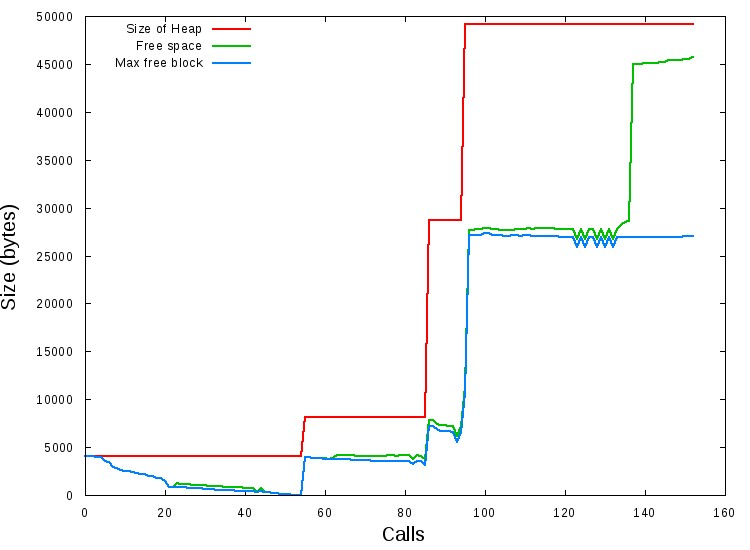
\includegraphics[width=1\linewidth]{Shashkova/images/size_zip_worst.jpg}}
   \caption{Состояние кучи с аллокаторм Worst fit и мутатором zip}
   \label{ris:image}
   \end{figure}
   
   Можно отметить резкий скачок, а затем резкое уменьшение фрагментации в районе 60-го запроса. Для объяснения такого поведения, рассмотрим график размера кучи, 
   например, для аллокатора Worst fit(см. Рис. 2). На нем представлены размер кучи, размер свободного пространства в куче и величина максимального свободного
   блока.
   Тогда становится понятным, что резкое изменение фрагментации в районе 60-го запроса связано с увеличением размера кучи (добавляется большой свободный блок). 
   Подобное повторяется в районе 82-го и 98-го запросов, однако, там фрагментация изменяется не столь резко. Это связано с тем, что общий размер кучи к тому моменту
   уже значительно увеличился.
   
   
   \begin{figure}[p]
   \center{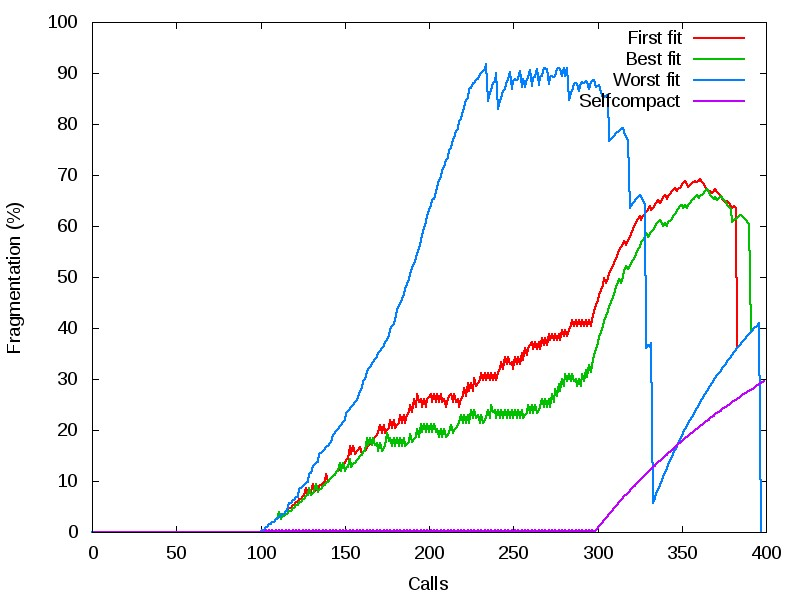
\includegraphics[width=1\linewidth]{Shashkova/images/fragment_list_selfcomp.jpg}}
   \caption{Величина фрагментации с мутатором sort list}
   \label{ris:image}
   \end{figure}
   
   На Рис. 3 представлена величина фрагментации в процессе исполнения программы --- сортировки связного списка --- для четырех аллокаторов. На первом участке графика
   видно, что для всех аллокатором величина фрагментации равна 0. На этом участке список создается, объекты располагаются в куче последовательно и все свободное
   пространство является одним блоком. 
   
   Затем, в процессе сортировки, некоторые объекты удаляются, под новые выделяется память. Здесь сразу можно заметить, что фрагментация алгоритма Worst fit растет
   быстрее фрагментации других алгоритмов. Около 300-го запроса можно отметить увеличение фрагментации у алгоритмов First fit и Best fit. 
   
   \begin{figure}[p]
   \center{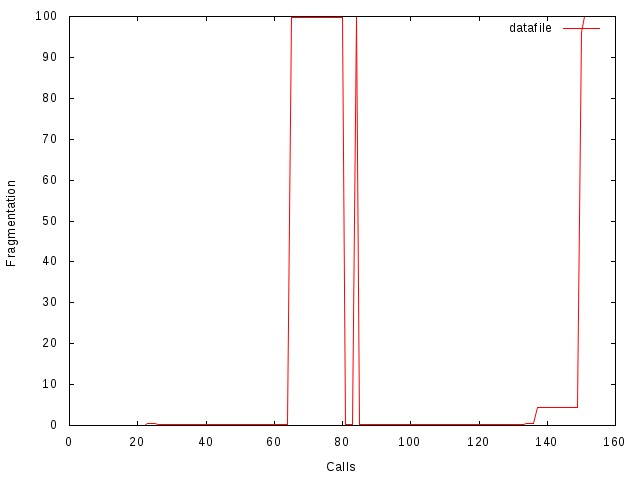
\includegraphics[width=1\linewidth]{Shashkova/images/fragment_bad.jpg}}
   \caption{Величина фрагментации аллокатора First fit}
   \label{ris:image}
   \end{figure}
   
    Хочется отметить, что сбор статистики помог выявить ошибку в первоначальной реализации аллокатора First fit. На Рис. 4 представлено, как изменялась фрагментация
   на одной из первых тестовых программ. 
   Такое резкое изменение фрагментации показалось нам неестественным. Благодаря этому была проведена перепроверка реализации и 
   выявлена ошибка.
   
   \begin{figure}[p]
   \center{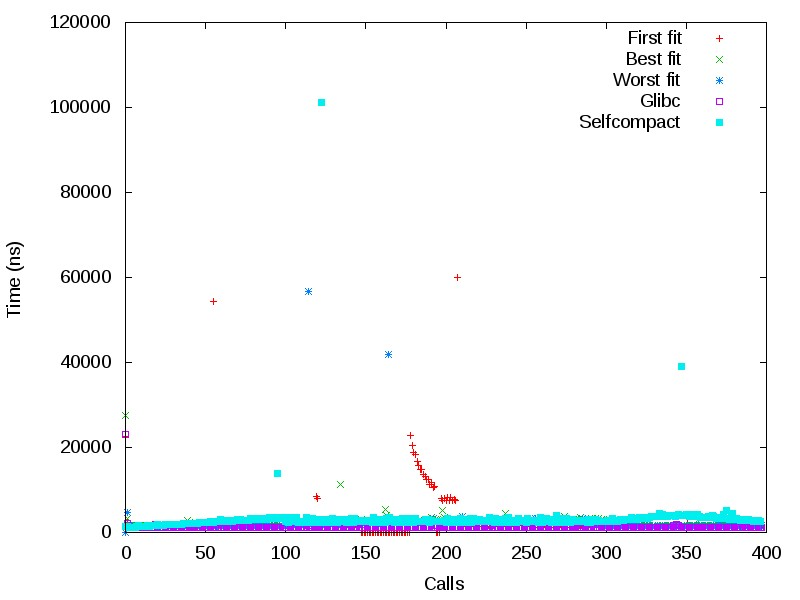
\includegraphics[width=1\linewidth]{Shashkova/images/time_gettime.jpg}}
   \caption{Время выполнения запросов}
   \label{ris:image}
   \end{figure}
   
   Также для различных алгоритмов измерялось время, затраченное аллокаторами на выполнение запросов. На Рис. 5 представлены результаты измерения времени в процессе
   работы программы. Можно заметить, что при некоторых запросах, время в несколько раз превышает среднее время на выделение. Это происходит на запросах о 
   выделении памяти, и, вероятно, это связано с поиском подходящего свободного блока. 
   
   \begin{figure}[p]
   \center{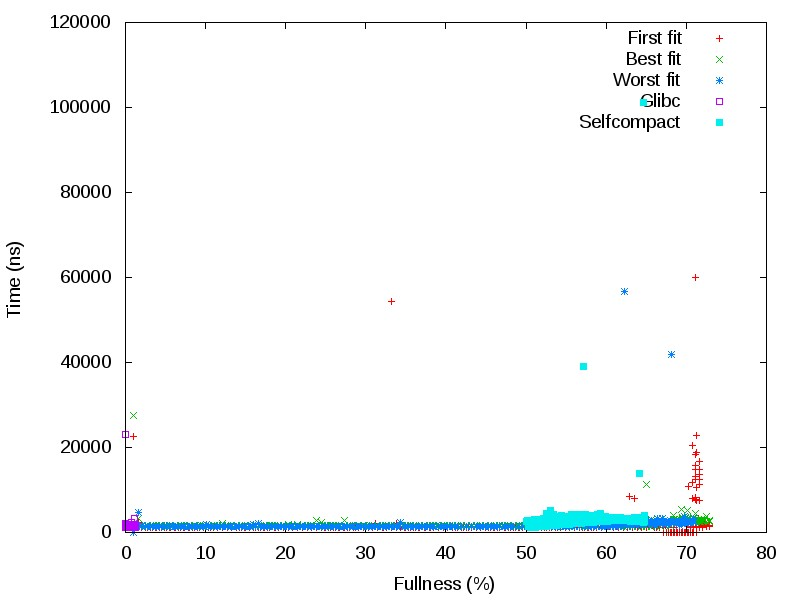
\includegraphics[width=1\linewidth]{Shashkova/images/time_full_self.jpg}}
   \caption{Зависимость времени выполнения запросов от заполненности кучи}
   \label{ris:image}
   \end{figure}
   
   \begin{figure}[p]
   \center{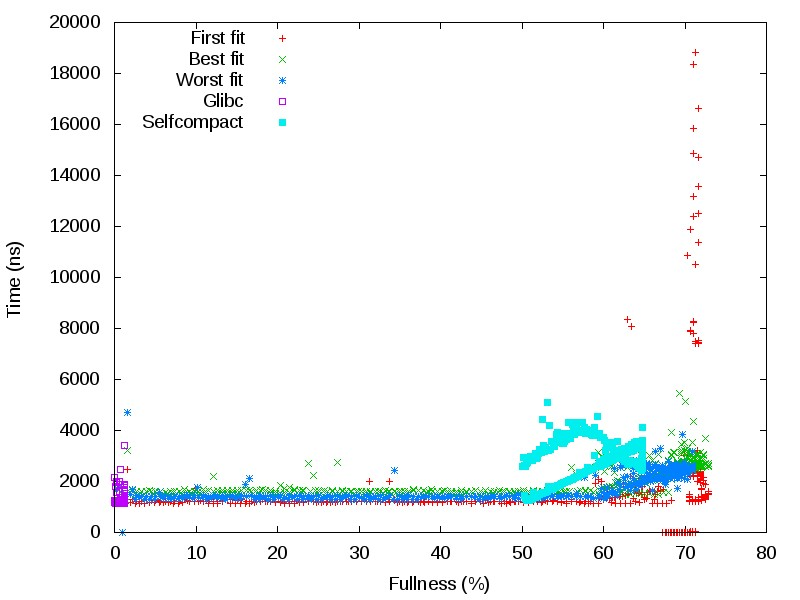
\includegraphics[width=1\linewidth]{Shashkova/images/time_full_zoom_3.jpg}}
   \caption{Зависимость времени выполнения запросов от заполненности кучи, увеличенный масштаб}
   \label{ris:image}
   \end{figure}
   
   На Рис. 6 представлена зависимость времени выделения от заполненности кучи. Наиболее выражена эта зависимость для алгоритма First fit. На Рис. 7 изображена та же
   зависимость с увеличенным масштабом для нижней части графика. На нём видно, что время выполнения запросов у самосжимающейся кучи больше, чем у остальных 
   алгоритмов. Также у всех алгоритмов наблюдается увеличение времени выполнения запросов с приближением заполненности кучи к наибольшему значению.
   
   
   \section{Заключение}
   
   В результате работы над данной курсовой работой:
   
    \begin{itemize}
     \item были изучены существующие метрики для сравнения реализаций кучи;
     \item были изучены подходы для проведения измерений;
     \item была создана система сравнения различных реализаций;
     \item была выявлена ошибка в реализации кучи.
    \end{itemize}

\begin{thebibliography}{99}
\bibitem{six_progs}
Benjamin Zorn, Dirk Grunwald.
Empirical Measurements of Six Allocation-intensive C Programs. University of Colorado, Boulder, 1992.

\bibitem{fragm}
Mark S. Johnstone, Paul R. Wilson.
The Memory Fragmentation Problem: Solved? The University of Texas at Austin, 1997.

\bibitem{un_mutator}
Martin Aigner, Christoph M. Kirsch. Towards a Universal Mutator for Benchmarking Heap Management Systems.
University of Salzburg, 2012.

\bibitem{ae}
James R. Larus. Abstract Execution: a Technique for Efficiently Tracing Programs.
Software --- Practice and Experience.

\bibitem{samofal}
Самофалов А.В. Способы реализации кучи и их свойства // Наст. сборник
\end{thebibliography}

%\documentclass[12pt,a4paper]{article}
%\usepackage[utf8x]{inputenc}
%\usepackage[russian]{babel}
%\usepackage[OT1]{fontenc}
%\usepackage{amsmath}
%\usepackage[a4paper,includeheadfoot,top=20mm,bottom=20mm,left=25mm,right=15mm]{geometry}
%\usepackage{indentfirst}
%\usepackage{amsfonts}
%\usepackage{amssymb}
%\usepackage{graphicx}
%\renewcommand\baselinestretch{1.5}
%\renewcommand\contentsname{Оглавление}

%\begin{document}
%\begin{titlepage}
%\thispagestyle{empty}
%\def\baselinestretch{1.0}
%\begin{center}
%	{\large САНКТ-ПЕТЕРБУРГСКИЙ ГОСУДАРСТВЕННЫЙ УНИВЕРСИТЕТ \\ \vskip 0.3em {\large Математико-механический факультет \\ \vskip 0.7em{\large Кафедра системного программирования \\}}}
%    \vspace*{0.15\textheight}
%    \vfill
%    {\large Шашкова Елизавета Михайловна}
%    
%    \vskip 2em
%    {\huge Методы профилирования реализаций кучи}
%    
%    \vskip 1em
%    {\large Курсовая работа} \\
%    \vskip 2em
%    {\normalsize \raggedleft 
%    Научный руководитель:\\
%    к.ф.-м.н. Д.Ю. Булычев
%    \\[3em]
%    \vspace*{0.08\textheight}
%    \vfill
%    {\centering Санкт-Петербург \\ 2013}
%    }
%\end{center}
%\end{titlepage}

\title{Методы профилирования реализаций кучи}
%
\titlerunning{Методы профилирования реализаций кучи}
\author{Шашкова Елизавета Михайловна}
%
\authorrunning{Е.М.Шашкова} % abbreviated author list (for running head)
%
%%%% list of authors for the TOC (use if author list has to be modified)
\tocauthor{Е.М.Шашкова}
%
\institute{Санк-Петербургский государственный университет\\
\email{Elizaveta239@yandex.ru}}

\maketitle              % typeset the title of the contribution

\begin{abstract}
\end{abstract}
%

\section*{Введение}

   Динамическое управление памятью --- это управление памятью для объектов, ни размер, ни время жизни которых, вообще говоря, неизвестны до
   выполнения программы. Под объектом мы будем понимать некоторый неделимый набор байт.
   
   Обычно при динамическом управлении памятью место под объекты выделяется в специальной области памяти --- \textquotedblleft куче\textquotedblright
   (heap). Существует
   две основных операции для управления памятью в куче: выделение памяти и освобождение. При выделении посылается запрос, в котором указывается количество
   требуемой памяти. При успешном выделении память изымается из кучи, то есть становится недоступна для последующего выделения.
   Освобождение памяти, наоборот, делает часть кучи доступной для последующего выделения.
   
   Поведение динамической памяти удобно описывать в терминах взаимодействия двух основных сущностей: \emph{аллокатора} и \emph{мутатора}. Аллокатор принимает запросы на выделение
   памяти в куче и её освобождение. Мутатор посылает данные запросы. Каждый запрос содержит количество памяти для выделения, причем 
   это количество, вообще говоря, становится известно только в момент исполнения программы.
   
   Эффективность работы программы во многом зависит от эффективности аллокатора. На сегодняшний момент существует много способов его 
   реализации; более того, развитие технологий стимулирует создание новых подходов. Поэтому становится важной задача уметь сравнивать разные
   реализации аллокаторов, находить наиболее подходящие реализации в данном конкретном случае.
   
   Для описания свойств аллокатора можно выделить два полярных подхода:
   \begin{enumerate}
   \item Рассмотрение свойств кучи с точки зрения поведения мутатора. Задача: определить, для какого класса программ данная реализация аллокатора 
   подойдет лучше всего. 
   \item Сравнительный анализ нескольких реализаций аллокатора. Задача: провести сравнение двух или нескольких аллокаторов при взаимодействии с
   одним и тем же мутатором.
   \end{enumerate}
   
   Основные свойства, которыми можно описать аллокатор в первом подходе:
   \begin{itemize}
   \item Суммарное количество выделенной памяти (в байтах и блоках).
   \item Наибольшее количество единовременно выделенной памяти за все время работы программы (в байтах и блоках).
   \item Среднее время жизни блока (в байтах). Это время вычисляется, как количество байт, помещенных в кучу за промежуток времени между 
   созданием и удалением объекта, поделенное на размер объекта (среднее время жизни одного байта в куче).
   \end{itemize}
   
   Основные свойства, которыми можно описать аллокатор во втором подходе:
   \begin{itemize}
   \item Фрагментация. Фрагментация вычисляется по следующей формуле: \[ F = \frac{free - free_{max}}{free} \]
   где $free$ --- количество свободных байт в куче, $free_{max}$ --- размер (в байтах) наибольшего свободного блока.  Так как память в куче выделяется
   блоками (наборами байтов), может так случиться, что в куче не осталось места для блока требуемого размера, хотя количество свободной 
   памяти еще превышает размер этого блока. С помощью данной формулы фрагментацию можно описать численной величиной. Чем меньше эта
   величина, тем \textquotedblleft лучше\textquotedblright~текущее состояние кучи. Фрагментации равна нулю, когда свободное место в 
   куче является одним блоком, и приближается к единице, когда размеры всех свободных блоков в куче малы. 
   \item Время выделения (в единицах времени).
   \item Порог работоспособности (количество запросов, обработанных аллокатором).
   \item Зависимость скорости работы аллокатора от нагрузки.
   \end{itemize}
    
   Цель данной курсовой работы заключается в том, чтобы изучить методы оценки реализации аллокатора. Необходимо понять, насколько 
   эффективно использование того или иного аллокатора, определить критерии, по которым различные аллокаторы будут сравниваться. В 
   соответствии с основными подходами, нужно сравнить поведение одного аллокатора при использовании нескольких различных мутаторов, а также
   сравнить поведение нескольких аллокаторов при работе с одним мутатором. В результате будет создан прототип системы для проведения 
   вышеуказанных сравнений.
   
   
   \section{Существующие подходы и метрики}
   Для сравнения различных реализаций аллокаторов прежде всего нужно выбрать метрики, по которым будет 
   производиться сравнение. Требуется понять, какие данные нужно собирать при запуске программ
   с использованием различных аллокаторов.
   
   В статье ~\cite{six_progs} представлены опытные данные, полученные с помощью шести программ на языке
   C. Авторы запустили каждую программу на нескольких наборах входных данных и построили распределения для следующих величин:
   
   \begin{itemize}
   \item размеров объектов;
   \item времён жизни объектов;
   \item интервалов времени между запросами.
   \end{itemize}
   
   Для этих распределений были найдены среднее, медиана и мода, которые характеризуют асимметричность распределения. Распределение размеров 
   объектов оказалось асимметричным 
   в сторону маленьких размеров: большая часть объектов, под которые выделялась память, имели размер менее 64 байт. Интересным
   оказался тот факт, что 90\% объектов имеют всего 10 различных размеров. Распределение времени жизни
   объектов показало, что большинство объектов живет в течение короткого промежутка времени: 40-80 машинных инструкций процессора 
   
   Данные об использовании памяти были получены посредством трассировки с помощью методики abstract execution~\cite{ae}. В качестве 
   тестовых программ для измерения были взяты: программа, находящая факториал больших целых чисел; оптимизатор Espresso; 
   GhostScript\footnote{http://www.ghostscript.com/} –-- интерпретатор языка PostScript; Gnu Awk\footnote{http://www.gnu.org/software/gawk/} –-- 
   интерпретатор языка AWK; интерпретатор Perl\footnote{http://www.perl.org/}; Chameleon –-- канальный роутер N-го уровня.
   
   Такой способ анализа аллокаторов нельзя полностью отнести ни к первому, ни ко второму подходу, т.к. в программах аллокатор и мутатор
   были фиксированными, изменялись только входные данные. Приоритетом для авторов являлось исследование свойств объектов, для которых выделяется
   память, а не аллокаторов.
   
   В статье ~\cite{fragm} авторы анализировали выделение памяти в нескольких приложениях, чтобы показать, что фрагментацию
   во время исполнения программы можно уменьшить посредством правильного выбора аллокатора. Было показано, что объекты,
   которые помещаются в кучу одновременно, удаляются из неё также одновременно. 
   Параметры, измерявшиеся в процессе работы программ, были таковы:
   
   \begin{itemize}
      \item время работы;
      \item суммарное количество выделенных объектов и байт;
      \item средний размер объектов;
      \item наибольшее количество объектов и байт, одновременно находящихся в куче;
      \item среднее время жизни объектов (в байтах).
   \end{itemize}
   
   Также, как и в предыдущей статье, было показано, что динамические объекты имеют обычно несколько определенных размеров. Был сделан
   вывод, что для уменьшения фрагментации при создании системы выделения памяти нужно опираться прежде всего на данное свойство программ.
   
   В данном исследовании авторы использовали как первый, так и второй подход. Они измеряли фрагментацию по всевозможным комбинациям имеющихся 
   у них мутаторов и аллокаторов.
   
   В ~\cite{un_mutator} авторы описывают созданный ими универсальный мутатор --- ACDC Benchmark Tool. Он представляет собой измеритель, 
   который может эмулировать выделение и очистку памяти и показывать различия между реализациями аллокаторов. Основная идея, заложенная в данном 
   измерителе, заключается в том, чтобы рассматривать в качестве метрики время и измерять его в байтах. Это было сделано для работы не только с
   однопоточными, но и с многопоточными мутаторами. 
   
   С помощью данного инструмента можно осуществить измерения в рамках как первого, так и второго подхода.
   
   
   \section{Проведение измерений}
   В данной работе были реализованы оба подхода к сбору данных. Для первого подхода, который заключается в рассмотрении свойств аллокатора с точки зрения мутатора, измерялись следующие величины:
   \begin{itemize}
      \item суммарное количество выделенной памяти (в байтах и блоках);
      \item наибольшее количество единовременно выделенной памяти за все время работы программы (в байтах и блоках);
      \item среднее время жизни блока (в байтах).
   \end{itemize}
      
   Для второго подхода, основная цель которого --- сравнить аллокаторы с использованием одного мутатора, 
   измерялись:
   \begin{itemize}
         \item фрагментация; 
         \item время выделения (в единицах времени);
         \item порог работоспособности (количество запросов, обработанных аллокатором);
         \item зависимость скорости работы аллокатора от нагрузки.
   \end{itemize}
      
   \subsection{Аллокаторы и мутаторы}
   
   Сбор данных производился как со стандартной реализации аллокатора в glibc, так и с собственной реализации,
   созданной Самофаловым А.В. ~\cite{samofal}. В его работе было реализовано несколько аллокаторов с различными алгоритмами
   выделения памяти.
   
   Эти алгоритмы:
   \begin{itemize}
      \item \textquotedblleft First fit\textquotedblright --- память выделяется в первом свободном блоке;
      \item \textquotedblleft Best fit\textquotedblright --- память выделяется в наиболее подходящем блоке;
      \item \textquotedblleft Worst fit\textquotedblright --- память выделяется в самом большом свободном блоке;
      \item \textquotedblleft Selfcompact\textquotedblright --- cамосжимающаяся куча.
   \end{itemize}
   
   В качестве мутаторов были взяты следующие программы:
   \begin{itemize}
        \item архиватор zip\footnote{http://www.info-zip.org};
   	    \item программа, сортирующая связный список --- sort list;
   	    \item архиватор tar\footnote{http://www.gnu.org/software/tar/}.
   \end{itemize}
   
   \subsection{Подробности реализации}
   
   В стандартной библиотеке языка C существует специальная структура \texttt{mallinfo}, которая описывает состояние кучи. Данная структура имеет следующие поля: 
   \begin{itemize}
   	     \item \texttt{int arena} --- суммарное пространство, выделенное под кучу (в байтах).
         \item \texttt{int ordblks} --- количество свободных блоков.
         \item \texttt{int smblks} --- количество свободных блоков \textquotedblleft fastbin\textquotedblright. Это блоки, которые были освобождены,
         однако, не были объединены с соседними свободными блоками. В этих блоках впоследствии можно 
         выделять память под объекты такого же размера.
          \item \texttt{int hblks} --- суммарное количество блоков, находящихся в куче.
          \item \texttt{int hblkhd} --- суммарное место, выделенное под блоки (в байтах).
          \item \texttt{int usmblks} --- наибольшее количество байт, находящихся в куче за время работы программы.
          \item \texttt{int fsmblks} --- суммарное место в блоках \textquotedblleft fastbin\textquotedblright (в байтах).
          \item \texttt{int uordblks} --- суммарное занятое пространство (в байтах).
          \item \texttt{int fordblks} --- суммарное свободное пространство (в байтах).
          \item \texttt{int keepcost} --- наибольшее количество пространства, которое можно освободить в начале кучи 
          (то есть посредством функции \texttt{malloc\_trim}) (в байтах).
   \end{itemize}
   
   Функция \texttt{mallinfo} возвращает копию структуры \texttt{mallinfo}. С её помощью были измерены некоторые величины для стандартной реализации аллокатора. 
   Для осуществления измерений были использованы hook-функции. Переменные \texttt{\_\_malloc\_hook}, \texttt{\_\_realloc\_hook} и \texttt{\_\_free\_hook} являются 
   указателями на функции, которые используют функции \texttt{malloc}, \texttt{realloc} и \texttt{free} соответственно всякий раз, когда они вызываются. Таким 
   образом можно привязывать вызов требуемых функций (в нашем случае --- сбор статистики) к запросам на выделение или очистку памяти.
   
   В собственной реализации для сбора статистики был создан аналог структуры \texttt{mallinfo} --- структура \texttt{myinfo}.
   Её устройство схоже с устройством \texttt{mallinfo}, однако, имеются некоторые различия. Она содержит следующие поля:
   \begin{itemize}
     \item \texttt{int arena} --- суммарное пространство, выделенное под кучу (в байтах);
     \item \texttt{int freemem} --- свободное пространство (в байтах);
     \item \texttt{int usdmem} --- занятое пространство (в байтах);
     \item \texttt{int freeblks} --- количество свободных блоков;
     \item \texttt{nt usdblks} --- количество используемых блоков;
     \item \texttt{maxfreeblk} --- размер наибольшего свободного блока (в байтах).
   \end{itemize} 
   
   Основным отличием данной структуры от структуры \texttt{mallinfo} является наличие поля с размером наибольшего свободного
   блока. Оно позволяет напрямую использовать это значение для вычисления фрагментации (по формуле, упоминавшейся
   во введении).
   
   
   \section{Результаты}
   
   Результаты измерений в первом подходе --- данные, усредненные по выполнению программы. Результаты представлены в следующих таблицах. Max(bytes) обозначает
   наибольшее количество единовременно выделенной памяти(в байтах). Sum(bytes) обозначает общее количество выделенной памяти(в байтах). Mean lifetime(bytes)
   обозначает среднее время жизни блока(в байтах).
    
    First fit:
    \begin{center}
    \begin{tabular}{| l | c | c | c | c | c |}
    \hline
    Мутатор & Max(bytes) & Max(blocks) & Sum(bytes) & Sum(blocks) & Mean lifetime(bytes)\\
    \hline
    zip & 21064 & 53 & 25845 & 77 & 1068.48\\
    \hline
    sort list & 808 & 101 & 1592 & 199 & 82.21 \\
    \hline
    tar & 52080 & 238 & 58736 & 404 & 446.86 \\
    \hline
    \end{tabular}
    \end{center}

    Best fit:
    \begin{center}
    \begin{tabular}{| l | c | c | c | c | c |}
    \hline
    Мутатор & Max(bytes) & Max(blocks) & Sum(bytes) & Sum(blocks) & Mean lifetime(bytes)\\
    \hline
    zip & 21080 & 53 & 25845 & 75 & 1068.64\\
    \hline
    sort list & 808 & 101 & 1592 & 199 & 82.27 \\
    \hline
    tar & 52112 & 238 & 58736 & 402 & 451.89 \\
    \hline
    \end{tabular}
    \end{center}
    
    Worst fit:
    \begin{center}
    \begin{tabular}{| l | c | c | c | c | c |}
    \hline
    Мутатор & Max(bytes) & Max(blocks) & Sum(bytes) & Sum(blocks) & Mean lifetime(bytes)\\
    \hline
    zip & 21064 & 53 & 25845 & 80 & 1069.85\\
    \hline
    sort list & 808 & 101 & 1592 & 199 & 80.72\\
    \hline
    tar & 52080 & 238 & 58736 & 404 & 455.58 \\
    \hline
    \end{tabular}
    \end{center}
    
   Средние величины для всех аллокаторов получились почти одинаковые. Данный подход к изучению аллокаторов не выявил их различий и особенностей.
    
   
   Во втором подходе измерения и сравнения производились после каждого запроса, которыми обменивались между собой аллокатор и мутатор. В связи с этим,
   полученные данные удобно представить в виде графиков.
   
   На Рис. 1 представлено изменение фрагментации для алгоритмов First fit, Best fit и Worst fit при работе с программой zip. Из пяти возможных аллокаторов
   величину фрагментации с мутатором zip удалось найти только для данных трех. Это связано с тем, что для стандартной реализации аллокатора фрагментацию по нашей
   формуле найти не удастся, так как нет возможности узнать размер наибольшего свободного блока. А аллокатор selfcompact требует специфичного написания мутатора и 
   его компиляции, поэтому запустить этот аллокатор с мутатором zip не представляется возможным.
   
   \begin{figure}[h]
   \center{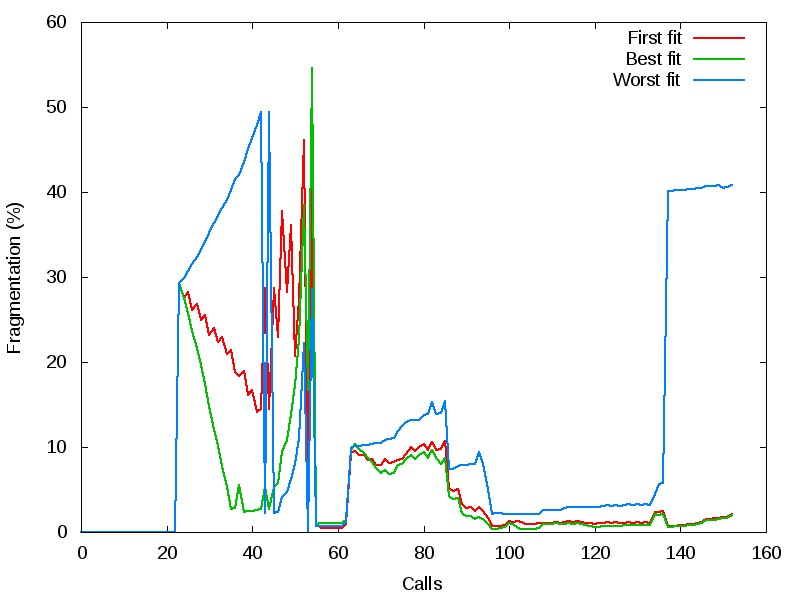
\includegraphics[width=1\linewidth]{Shashkova/images/fragment_zip.jpg}}
   \caption{Величина фрагментации с мутатором zip}
   \label{ris:image}
   \end{figure}
   
   Можно заметить, что первом участке у всех трех аллокаторов величина фрагментации равна 0. Это связано с тем, что освобождения памяти еще не производились и объекты
   находятся в куче последовательно, без пропусков. Затем фрагментация начинает возрастать. Как и предполагалось теоретически, почти на всех участках графика 
   фрагментация аллокатора Worst fit больше фрагментации остальных аллокаторов, а фрагментация аллокатора Best fit меньше фрагментации остальных аллокаторов.
   
   \begin{figure}[p]
   \center{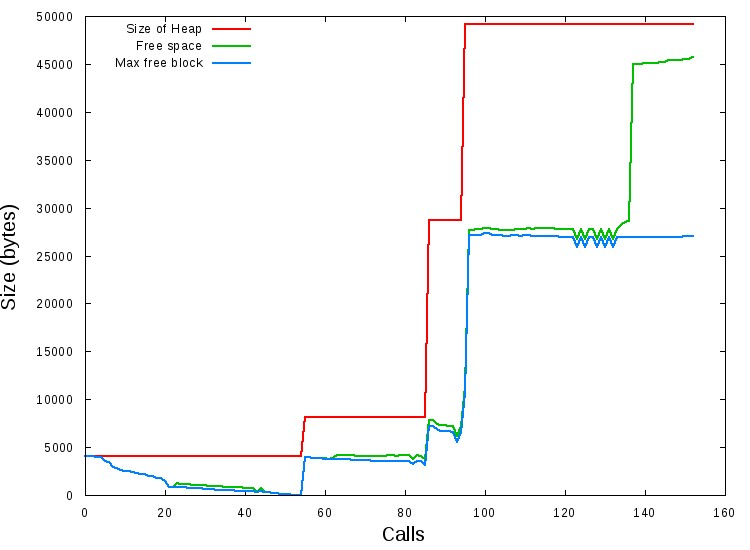
\includegraphics[width=1\linewidth]{Shashkova/images/size_zip_worst.jpg}}
   \caption{Состояние кучи с аллокаторм Worst fit и мутатором zip}
   \label{ris:image}
   \end{figure}
   
   Можно отметить резкий скачок, а затем резкое уменьшение фрагментации в районе 60-го запроса. Для объяснения такого поведения, рассмотрим график размера кучи, 
   например, для аллокатора Worst fit(см. Рис. 2). На нем представлены размер кучи, размер свободного пространства в куче и величина максимального свободного
   блока.
   Тогда становится понятным, что резкое изменение фрагментации в районе 60-го запроса связано с увеличением размера кучи (добавляется большой свободный блок). 
   Подобное повторяется в районе 82-го и 98-го запросов, однако, там фрагментация изменяется не столь резко. Это связано с тем, что общий размер кучи к тому моменту
   уже значительно увеличился.
   
   
   \begin{figure}[p]
   \center{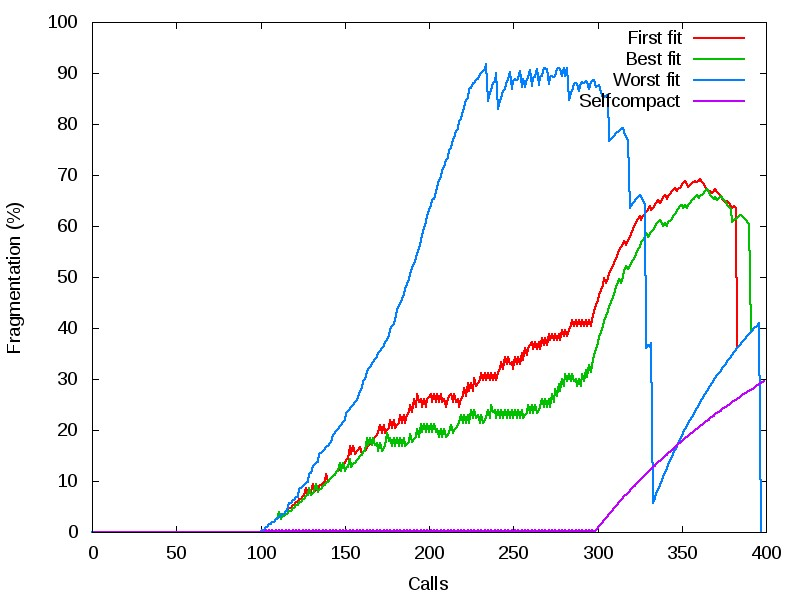
\includegraphics[width=1\linewidth]{Shashkova/images/fragment_list_selfcomp.jpg}}
   \caption{Величина фрагментации с мутатором sort list}
   \label{ris:image}
   \end{figure}
   
   На Рис. 3 представлена величина фрагментации в процессе исполнения программы --- сортировки связного списка --- для четырех аллокаторов. На первом участке графика
   видно, что для всех аллокатором величина фрагментации равна 0. На этом участке список создается, объекты располагаются в куче последовательно и все свободное
   пространство является одним блоком. 
   
   Затем, в процессе сортировки, некоторые объекты удаляются, под новые выделяется память. Здесь сразу можно заметить, что фрагментация алгоритма Worst fit растет
   быстрее фрагментации других алгоритмов. Около 300-го запроса можно отметить увеличение фрагментации у алгоритмов First fit и Best fit. 
   
   \begin{figure}[p]
   \center{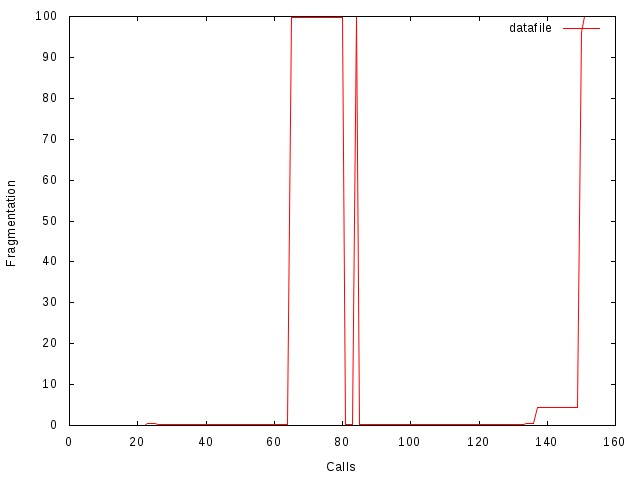
\includegraphics[width=1\linewidth]{Shashkova/images/fragment_bad.jpg}}
   \caption{Величина фрагментации аллокатора First fit}
   \label{ris:image}
   \end{figure}
   
    Хочется отметить, что сбор статистики помог выявить ошибку в первоначальной реализации аллокатора First fit. На Рис. 4 представлено, как изменялась фрагментация
   на одной из первых тестовых программ. 
   Такое резкое изменение фрагментации показалось нам неестественным. Благодаря этому была проведена перепроверка реализации и 
   выявлена ошибка.
   
   \begin{figure}[p]
   \center{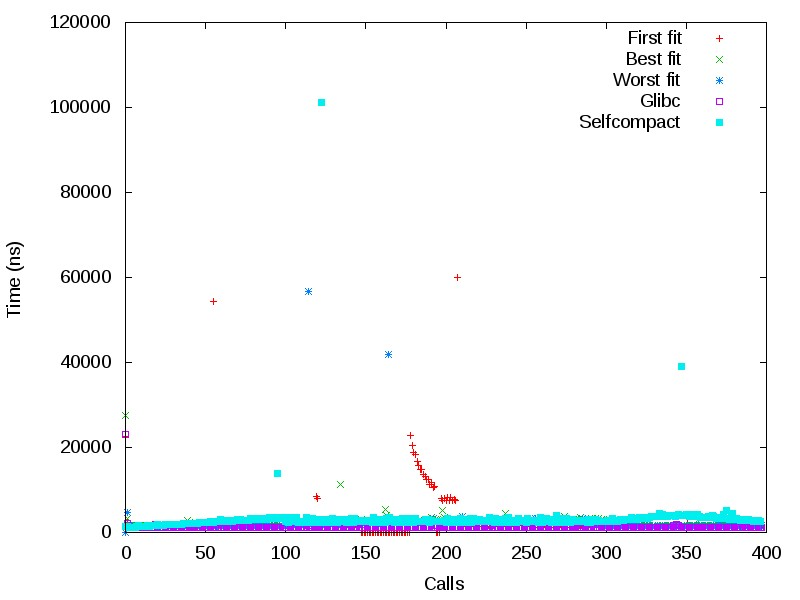
\includegraphics[width=1\linewidth]{Shashkova/images/time_gettime.jpg}}
   \caption{Время выполнения запросов}
   \label{ris:image}
   \end{figure}
   
   Также для различных алгоритмов измерялось время, затраченное аллокаторами на выполнение запросов. На Рис. 5 представлены результаты измерения времени в процессе
   работы программы. Можно заметить, что при некоторых запросах, время в несколько раз превышает среднее время на выделение. Это происходит на запросах о 
   выделении памяти, и, вероятно, это связано с поиском подходящего свободного блока. 
   
   \begin{figure}[p]
   \center{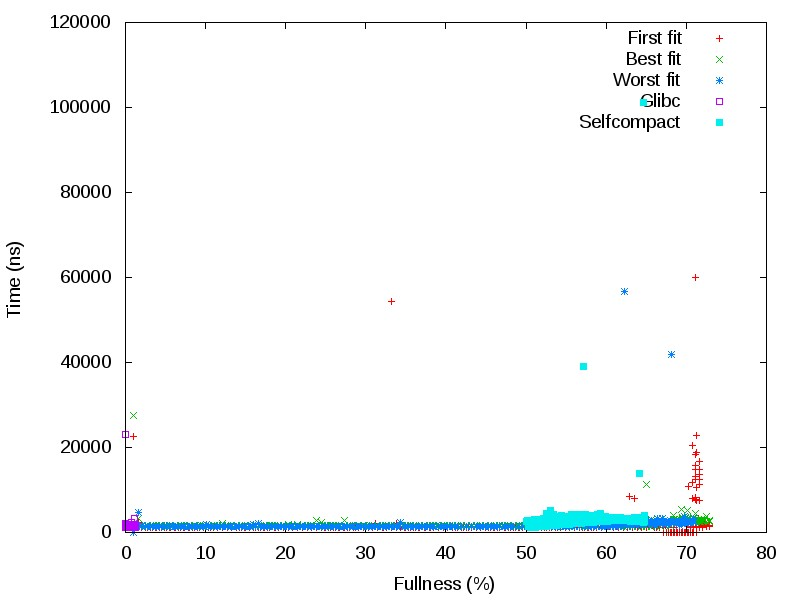
\includegraphics[width=1\linewidth]{Shashkova/images/time_full_self.jpg}}
   \caption{Зависимость времени выполнения запросов от заполненности кучи}
   \label{ris:image}
   \end{figure}
   
   \begin{figure}[p]
   \center{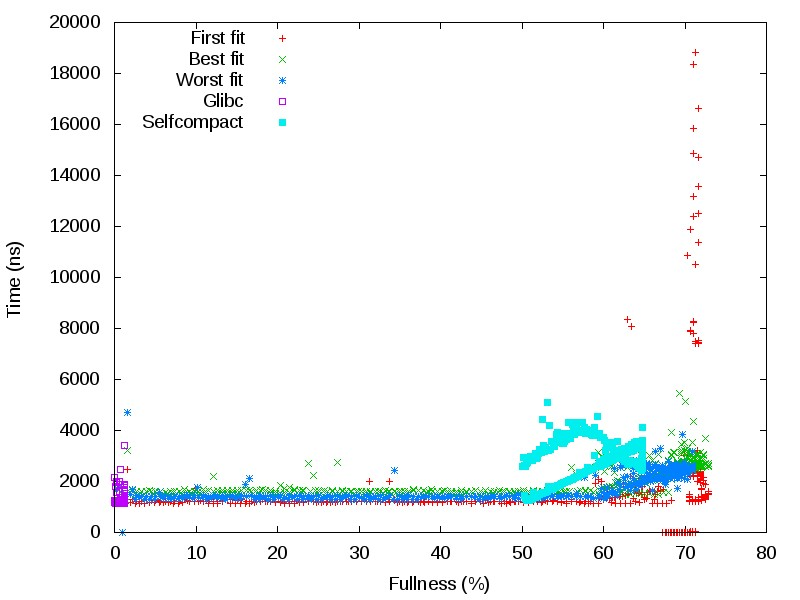
\includegraphics[width=1\linewidth]{Shashkova/images/time_full_zoom_3.jpg}}
   \caption{Зависимость времени выполнения запросов от заполненности кучи, увеличенный масштаб}
   \label{ris:image}
   \end{figure}
   
   На Рис. 6 представлена зависимость времени выделения от заполненности кучи. Наиболее выражена эта зависимость для алгоритма First fit. На Рис. 7 изображена та же
   зависимость с увеличенным масштабом для нижней части графика. На нём видно, что время выполнения запросов у самосжимающейся кучи больше, чем у остальных 
   алгоритмов. Также у всех алгоритмов наблюдается увеличение времени выполнения запросов с приближением заполненности кучи к наибольшему значению.
   
   
   \section{Заключение}
   
   В результате работы над данной курсовой работой:
   
    \begin{itemize}
     \item были изучены существующие метрики для сравнения реализаций кучи;
     \item были изучены подходы для проведения измерений;
     \item была создана система сравнения различных реализаций;
     \item была выявлена ошибка в реализации кучи.
    \end{itemize}

\begin{thebibliography}{99}
\bibitem{six_progs}
Benjamin Zorn, Dirk Grunwald.
Empirical Measurements of Six Allocation-intensive C Programs. University of Colorado, Boulder, 1992.

\bibitem{fragm}
Mark S. Johnstone, Paul R. Wilson.
The Memory Fragmentation Problem: Solved? The University of Texas at Austin, 1997.

\bibitem{un_mutator}
Martin Aigner, Christoph M. Kirsch. Towards a Universal Mutator for Benchmarking Heap Management Systems.
University of Salzburg, 2012.

\bibitem{ae}
James R. Larus. Abstract Execution: a Technique for Efficiently Tracing Programs.
Software --- Practice and Experience.

\bibitem{samofal}
Самофалов А.В. Способы реализации кучи и их свойства // Наст. сборник
\end{thebibliography}


%\documentclass[12pt,a4paper]{article}
%\usepackage[utf8x]{inputenc}
%\usepackage[russian]{babel}
%\usepackage[OT1]{fontenc}
%\usepackage{amsmath}
%\usepackage[a4paper,includeheadfoot,top=20mm,bottom=20mm,left=25mm,right=15mm]{geometry}
%\usepackage{indentfirst}
%\usepackage{amsfonts}
%\usepackage{amssymb}
%\usepackage{graphicx}
%\renewcommand\baselinestretch{1.5}
%\renewcommand\contentsname{Оглавление}

%\begin{document}
%\begin{titlepage}
%\thispagestyle{empty}
%\def\baselinestretch{1.0}
%\begin{center}
%	{\large САНКТ-ПЕТЕРБУРГСКИЙ ГОСУДАРСТВЕННЫЙ УНИВЕРСИТЕТ \\ \vskip 0.3em {\large Математико-механический факультет \\ \vskip 0.7em{\large Кафедра системного программирования \\}}}
%    \vspace*{0.15\textheight}
%    \vfill
%    {\large Шашкова Елизавета Михайловна}
%    
%    \vskip 2em
%    {\huge Методы профилирования реализаций кучи}
%    
%    \vskip 1em
%    {\large Курсовая работа} \\
%    \vskip 2em
%    {\normalsize \raggedleft 
%    Научный руководитель:\\
%    к.ф.-м.н. Д.Ю. Булычев
%    \\[3em]
%    \vspace*{0.08\textheight}
%    \vfill
%    {\centering Санкт-Петербург \\ 2013}
%    }
%\end{center}
%\end{titlepage}

\title{Методы профилирования реализаций кучи}
%
\titlerunning{Методы профилирования реализаций кучи}
\author{Шашкова Елизавета Михайловна}
%
\authorrunning{Е.М.Шашкова} % abbreviated author list (for running head)
%
%%%% list of authors for the TOC (use if author list has to be modified)
\tocauthor{Е.М.Шашкова}
%
\institute{Санк-Петербургский государственный университет\\
\email{Elizaveta239@yandex.ru}}

\maketitle              % typeset the title of the contribution

\begin{abstract}
\end{abstract}
%

\section*{Введение}

   Динамическое управление памятью --- это управление памятью для объектов, ни размер, ни время жизни которых, вообще говоря, неизвестны до
   выполнения программы. Под объектом мы будем понимать некоторый неделимый набор байт.
   
   Обычно при динамическом управлении памятью место под объекты выделяется в специальной области памяти --- \textquotedblleft куче\textquotedblright
   (heap). Существует
   две основных операции для управления памятью в куче: выделение памяти и освобождение. При выделении посылается запрос, в котором указывается количество
   требуемой памяти. При успешном выделении память изымается из кучи, то есть становится недоступна для последующего выделения.
   Освобождение памяти, наоборот, делает часть кучи доступной для последующего выделения.
   
   Поведение динамической памяти удобно описывать в терминах взаимодействия двух основных сущностей: \emph{аллокатора} и \emph{мутатора}. Аллокатор принимает запросы на выделение
   памяти в куче и её освобождение. Мутатор посылает данные запросы. Каждый запрос содержит количество памяти для выделения, причем 
   это количество, вообще говоря, становится известно только в момент исполнения программы.
   
   Эффективность работы программы во многом зависит от эффективности аллокатора. На сегодняшний момент существует много способов его 
   реализации; более того, развитие технологий стимулирует создание новых подходов. Поэтому становится важной задача уметь сравнивать разные
   реализации аллокаторов, находить наиболее подходящие реализации в данном конкретном случае.
   
   Для описания свойств аллокатора можно выделить два полярных подхода:
   \begin{enumerate}
   \item Рассмотрение свойств кучи с точки зрения поведения мутатора. Задача: определить, для какого класса программ данная реализация аллокатора 
   подойдет лучше всего. 
   \item Сравнительный анализ нескольких реализаций аллокатора. Задача: провести сравнение двух или нескольких аллокаторов при взаимодействии с
   одним и тем же мутатором.
   \end{enumerate}
   
   Основные свойства, которыми можно описать аллокатор в первом подходе:
   \begin{itemize}
   \item Суммарное количество выделенной памяти (в байтах и блоках).
   \item Наибольшее количество единовременно выделенной памяти за все время работы программы (в байтах и блоках).
   \item Среднее время жизни блока (в байтах). Это время вычисляется, как количество байт, помещенных в кучу за промежуток времени между 
   созданием и удалением объекта, поделенное на размер объекта (среднее время жизни одного байта в куче).
   \end{itemize}
   
   Основные свойства, которыми можно описать аллокатор во втором подходе:
   \begin{itemize}
   \item Фрагментация. Фрагментация вычисляется по следующей формуле: \[ F = \frac{free - free_{max}}{free} \]
   где $free$ --- количество свободных байт в куче, $free_{max}$ --- размер (в байтах) наибольшего свободного блока.  Так как память в куче выделяется
   блоками (наборами байтов), может так случиться, что в куче не осталось места для блока требуемого размера, хотя количество свободной 
   памяти еще превышает размер этого блока. С помощью данной формулы фрагментацию можно описать численной величиной. Чем меньше эта
   величина, тем \textquotedblleft лучше\textquotedblright~текущее состояние кучи. Фрагментации равна нулю, когда свободное место в 
   куче является одним блоком, и приближается к единице, когда размеры всех свободных блоков в куче малы. 
   \item Время выделения (в единицах времени).
   \item Порог работоспособности (количество запросов, обработанных аллокатором).
   \item Зависимость скорости работы аллокатора от нагрузки.
   \end{itemize}
    
   Цель данной курсовой работы заключается в том, чтобы изучить методы оценки реализации аллокатора. Необходимо понять, насколько 
   эффективно использование того или иного аллокатора, определить критерии, по которым различные аллокаторы будут сравниваться. В 
   соответствии с основными подходами, нужно сравнить поведение одного аллокатора при использовании нескольких различных мутаторов, а также
   сравнить поведение нескольких аллокаторов при работе с одним мутатором. В результате будет создан прототип системы для проведения 
   вышеуказанных сравнений.
   
   
   \section{Существующие подходы и метрики}
   Для сравнения различных реализаций аллокаторов прежде всего нужно выбрать метрики, по которым будет 
   производиться сравнение. Требуется понять, какие данные нужно собирать при запуске программ
   с использованием различных аллокаторов.
   
   В статье ~\cite{six_progs} представлены опытные данные, полученные с помощью шести программ на языке
   C. Авторы запустили каждую программу на нескольких наборах входных данных и построили распределения для следующих величин:
   
   \begin{itemize}
   \item размеров объектов;
   \item времён жизни объектов;
   \item интервалов времени между запросами.
   \end{itemize}
   
   Для этих распределений были найдены среднее, медиана и мода, которые характеризуют асимметричность распределения. Распределение размеров 
   объектов оказалось асимметричным 
   в сторону маленьких размеров: большая часть объектов, под которые выделялась память, имели размер менее 64 байт. Интересным
   оказался тот факт, что 90\% объектов имеют всего 10 различных размеров. Распределение времени жизни
   объектов показало, что большинство объектов живет в течение короткого промежутка времени: 40-80 машинных инструкций процессора 
   
   Данные об использовании памяти были получены посредством трассировки с помощью методики abstract execution~\cite{ae}. В качестве 
   тестовых программ для измерения были взяты: программа, находящая факториал больших целых чисел; оптимизатор Espresso; 
   GhostScript\footnote{http://www.ghostscript.com/} –-- интерпретатор языка PostScript; Gnu Awk\footnote{http://www.gnu.org/software/gawk/} –-- 
   интерпретатор языка AWK; интерпретатор Perl\footnote{http://www.perl.org/}; Chameleon –-- канальный роутер N-го уровня.
   
   Такой способ анализа аллокаторов нельзя полностью отнести ни к первому, ни ко второму подходу, т.к. в программах аллокатор и мутатор
   были фиксированными, изменялись только входные данные. Приоритетом для авторов являлось исследование свойств объектов, для которых выделяется
   память, а не аллокаторов.
   
   В статье ~\cite{fragm} авторы анализировали выделение памяти в нескольких приложениях, чтобы показать, что фрагментацию
   во время исполнения программы можно уменьшить посредством правильного выбора аллокатора. Было показано, что объекты,
   которые помещаются в кучу одновременно, удаляются из неё также одновременно. 
   Параметры, измерявшиеся в процессе работы программ, были таковы:
   
   \begin{itemize}
      \item время работы;
      \item суммарное количество выделенных объектов и байт;
      \item средний размер объектов;
      \item наибольшее количество объектов и байт, одновременно находящихся в куче;
      \item среднее время жизни объектов (в байтах).
   \end{itemize}
   
   Также, как и в предыдущей статье, было показано, что динамические объекты имеют обычно несколько определенных размеров. Был сделан
   вывод, что для уменьшения фрагментации при создании системы выделения памяти нужно опираться прежде всего на данное свойство программ.
   
   В данном исследовании авторы использовали как первый, так и второй подход. Они измеряли фрагментацию по всевозможным комбинациям имеющихся 
   у них мутаторов и аллокаторов.
   
   В ~\cite{un_mutator} авторы описывают созданный ими универсальный мутатор --- ACDC Benchmark Tool. Он представляет собой измеритель, 
   который может эмулировать выделение и очистку памяти и показывать различия между реализациями аллокаторов. Основная идея, заложенная в данном 
   измерителе, заключается в том, чтобы рассматривать в качестве метрики время и измерять его в байтах. Это было сделано для работы не только с
   однопоточными, но и с многопоточными мутаторами. 
   
   С помощью данного инструмента можно осуществить измерения в рамках как первого, так и второго подхода.
   
   
   \section{Проведение измерений}
   В данной работе были реализованы оба подхода к сбору данных. Для первого подхода, который заключается в рассмотрении свойств аллокатора с точки зрения мутатора, измерялись следующие величины:
   \begin{itemize}
      \item суммарное количество выделенной памяти (в байтах и блоках);
      \item наибольшее количество единовременно выделенной памяти за все время работы программы (в байтах и блоках);
      \item среднее время жизни блока (в байтах).
   \end{itemize}
      
   Для второго подхода, основная цель которого --- сравнить аллокаторы с использованием одного мутатора, 
   измерялись:
   \begin{itemize}
         \item фрагментация; 
         \item время выделения (в единицах времени);
         \item порог работоспособности (количество запросов, обработанных аллокатором);
         \item зависимость скорости работы аллокатора от нагрузки.
   \end{itemize}
      
   \subsection{Аллокаторы и мутаторы}
   
   Сбор данных производился как со стандартной реализации аллокатора в glibc, так и с собственной реализации,
   созданной Самофаловым А.В. ~\cite{samofal}. В его работе было реализовано несколько аллокаторов с различными алгоритмами
   выделения памяти.
   
   Эти алгоритмы:
   \begin{itemize}
      \item \textquotedblleft First fit\textquotedblright --- память выделяется в первом свободном блоке;
      \item \textquotedblleft Best fit\textquotedblright --- память выделяется в наиболее подходящем блоке;
      \item \textquotedblleft Worst fit\textquotedblright --- память выделяется в самом большом свободном блоке;
      \item \textquotedblleft Selfcompact\textquotedblright --- cамосжимающаяся куча.
   \end{itemize}
   
   В качестве мутаторов были взяты следующие программы:
   \begin{itemize}
        \item архиватор zip\footnote{http://www.info-zip.org};
   	    \item программа, сортирующая связный список --- sort list;
   	    \item архиватор tar\footnote{http://www.gnu.org/software/tar/}.
   \end{itemize}
   
   \subsection{Подробности реализации}
   
   В стандартной библиотеке языка C существует специальная структура \texttt{mallinfo}, которая описывает состояние кучи. Данная структура имеет следующие поля: 
   \begin{itemize}
   	     \item \texttt{int arena} --- суммарное пространство, выделенное под кучу (в байтах).
         \item \texttt{int ordblks} --- количество свободных блоков.
         \item \texttt{int smblks} --- количество свободных блоков \textquotedblleft fastbin\textquotedblright. Это блоки, которые были освобождены,
         однако, не были объединены с соседними свободными блоками. В этих блоках впоследствии можно 
         выделять память под объекты такого же размера.
          \item \texttt{int hblks} --- суммарное количество блоков, находящихся в куче.
          \item \texttt{int hblkhd} --- суммарное место, выделенное под блоки (в байтах).
          \item \texttt{int usmblks} --- наибольшее количество байт, находящихся в куче за время работы программы.
          \item \texttt{int fsmblks} --- суммарное место в блоках \textquotedblleft fastbin\textquotedblright (в байтах).
          \item \texttt{int uordblks} --- суммарное занятое пространство (в байтах).
          \item \texttt{int fordblks} --- суммарное свободное пространство (в байтах).
          \item \texttt{int keepcost} --- наибольшее количество пространства, которое можно освободить в начале кучи 
          (то есть посредством функции \texttt{malloc\_trim}) (в байтах).
   \end{itemize}
   
   Функция \texttt{mallinfo} возвращает копию структуры \texttt{mallinfo}. С её помощью были измерены некоторые величины для стандартной реализации аллокатора. 
   Для осуществления измерений были использованы hook-функции. Переменные \texttt{\_\_malloc\_hook}, \texttt{\_\_realloc\_hook} и \texttt{\_\_free\_hook} являются 
   указателями на функции, которые используют функции \texttt{malloc}, \texttt{realloc} и \texttt{free} соответственно всякий раз, когда они вызываются. Таким 
   образом можно привязывать вызов требуемых функций (в нашем случае --- сбор статистики) к запросам на выделение или очистку памяти.
   
   В собственной реализации для сбора статистики был создан аналог структуры \texttt{mallinfo} --- структура \texttt{myinfo}.
   Её устройство схоже с устройством \texttt{mallinfo}, однако, имеются некоторые различия. Она содержит следующие поля:
   \begin{itemize}
     \item \texttt{int arena} --- суммарное пространство, выделенное под кучу (в байтах);
     \item \texttt{int freemem} --- свободное пространство (в байтах);
     \item \texttt{int usdmem} --- занятое пространство (в байтах);
     \item \texttt{int freeblks} --- количество свободных блоков;
     \item \texttt{nt usdblks} --- количество используемых блоков;
     \item \texttt{maxfreeblk} --- размер наибольшего свободного блока (в байтах).
   \end{itemize} 
   
   Основным отличием данной структуры от структуры \texttt{mallinfo} является наличие поля с размером наибольшего свободного
   блока. Оно позволяет напрямую использовать это значение для вычисления фрагментации (по формуле, упоминавшейся
   во введении).
   
   
   \section{Результаты}
   
   Результаты измерений в первом подходе --- данные, усредненные по выполнению программы. Результаты представлены в следующих таблицах. Max(bytes) обозначает
   наибольшее количество единовременно выделенной памяти(в байтах). Sum(bytes) обозначает общее количество выделенной памяти(в байтах). Mean lifetime(bytes)
   обозначает среднее время жизни блока(в байтах).
    
    First fit:
    \begin{center}
    \begin{tabular}{| l | c | c | c | c | c |}
    \hline
    Мутатор & Max(bytes) & Max(blocks) & Sum(bytes) & Sum(blocks) & Mean lifetime(bytes)\\
    \hline
    zip & 21064 & 53 & 25845 & 77 & 1068.48\\
    \hline
    sort list & 808 & 101 & 1592 & 199 & 82.21 \\
    \hline
    tar & 52080 & 238 & 58736 & 404 & 446.86 \\
    \hline
    \end{tabular}
    \end{center}

    Best fit:
    \begin{center}
    \begin{tabular}{| l | c | c | c | c | c |}
    \hline
    Мутатор & Max(bytes) & Max(blocks) & Sum(bytes) & Sum(blocks) & Mean lifetime(bytes)\\
    \hline
    zip & 21080 & 53 & 25845 & 75 & 1068.64\\
    \hline
    sort list & 808 & 101 & 1592 & 199 & 82.27 \\
    \hline
    tar & 52112 & 238 & 58736 & 402 & 451.89 \\
    \hline
    \end{tabular}
    \end{center}
    
    Worst fit:
    \begin{center}
    \begin{tabular}{| l | c | c | c | c | c |}
    \hline
    Мутатор & Max(bytes) & Max(blocks) & Sum(bytes) & Sum(blocks) & Mean lifetime(bytes)\\
    \hline
    zip & 21064 & 53 & 25845 & 80 & 1069.85\\
    \hline
    sort list & 808 & 101 & 1592 & 199 & 80.72\\
    \hline
    tar & 52080 & 238 & 58736 & 404 & 455.58 \\
    \hline
    \end{tabular}
    \end{center}
    
   Средние величины для всех аллокаторов получились почти одинаковые. Данный подход к изучению аллокаторов не выявил их различий и особенностей.
    
   
   Во втором подходе измерения и сравнения производились после каждого запроса, которыми обменивались между собой аллокатор и мутатор. В связи с этим,
   полученные данные удобно представить в виде графиков.
   
   На Рис. 1 представлено изменение фрагментации для алгоритмов First fit, Best fit и Worst fit при работе с программой zip. Из пяти возможных аллокаторов
   величину фрагментации с мутатором zip удалось найти только для данных трех. Это связано с тем, что для стандартной реализации аллокатора фрагментацию по нашей
   формуле найти не удастся, так как нет возможности узнать размер наибольшего свободного блока. А аллокатор selfcompact требует специфичного написания мутатора и 
   его компиляции, поэтому запустить этот аллокатор с мутатором zip не представляется возможным.
   
   \begin{figure}[h]
   \center{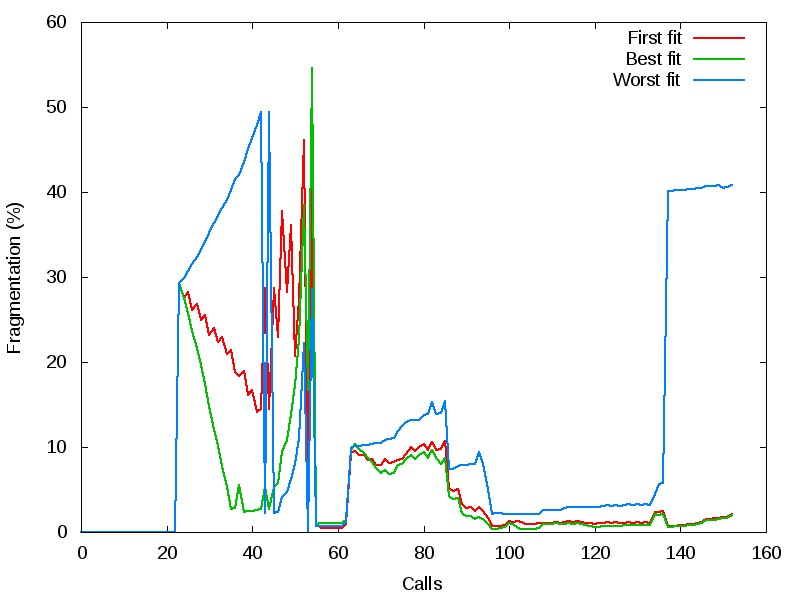
\includegraphics[width=1\linewidth]{Shashkova/images/fragment_zip.jpg}}
   \caption{Величина фрагментации с мутатором zip}
   \label{ris:image}
   \end{figure}
   
   Можно заметить, что первом участке у всех трех аллокаторов величина фрагментации равна 0. Это связано с тем, что освобождения памяти еще не производились и объекты
   находятся в куче последовательно, без пропусков. Затем фрагментация начинает возрастать. Как и предполагалось теоретически, почти на всех участках графика 
   фрагментация аллокатора Worst fit больше фрагментации остальных аллокаторов, а фрагментация аллокатора Best fit меньше фрагментации остальных аллокаторов.
   
   \begin{figure}[p]
   \center{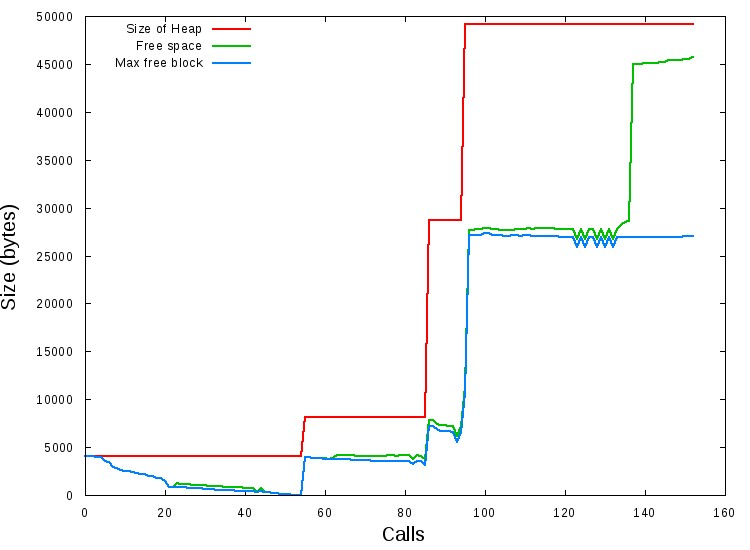
\includegraphics[width=1\linewidth]{Shashkova/images/size_zip_worst.jpg}}
   \caption{Состояние кучи с аллокаторм Worst fit и мутатором zip}
   \label{ris:image}
   \end{figure}
   
   Можно отметить резкий скачок, а затем резкое уменьшение фрагментации в районе 60-го запроса. Для объяснения такого поведения, рассмотрим график размера кучи, 
   например, для аллокатора Worst fit(см. Рис. 2). На нем представлены размер кучи, размер свободного пространства в куче и величина максимального свободного
   блока.
   Тогда становится понятным, что резкое изменение фрагментации в районе 60-го запроса связано с увеличением размера кучи (добавляется большой свободный блок). 
   Подобное повторяется в районе 82-го и 98-го запросов, однако, там фрагментация изменяется не столь резко. Это связано с тем, что общий размер кучи к тому моменту
   уже значительно увеличился.
   
   
   \begin{figure}[p]
   \center{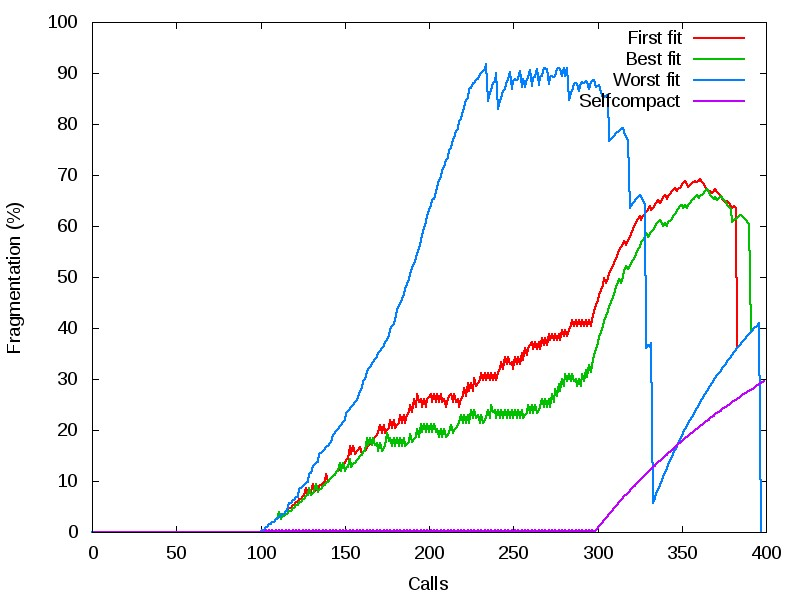
\includegraphics[width=1\linewidth]{Shashkova/images/fragment_list_selfcomp.jpg}}
   \caption{Величина фрагментации с мутатором sort list}
   \label{ris:image}
   \end{figure}
   
   На Рис. 3 представлена величина фрагментации в процессе исполнения программы --- сортировки связного списка --- для четырех аллокаторов. На первом участке графика
   видно, что для всех аллокатором величина фрагментации равна 0. На этом участке список создается, объекты располагаются в куче последовательно и все свободное
   пространство является одним блоком. 
   
   Затем, в процессе сортировки, некоторые объекты удаляются, под новые выделяется память. Здесь сразу можно заметить, что фрагментация алгоритма Worst fit растет
   быстрее фрагментации других алгоритмов. Около 300-го запроса можно отметить увеличение фрагментации у алгоритмов First fit и Best fit. 
   
   \begin{figure}[p]
   \center{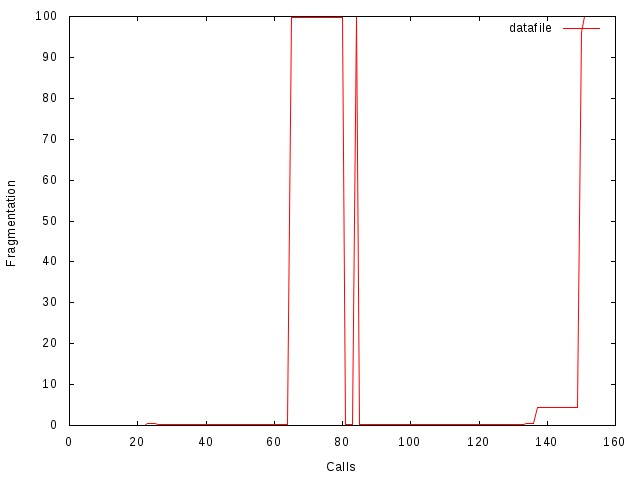
\includegraphics[width=1\linewidth]{Shashkova/images/fragment_bad.jpg}}
   \caption{Величина фрагментации аллокатора First fit}
   \label{ris:image}
   \end{figure}
   
    Хочется отметить, что сбор статистики помог выявить ошибку в первоначальной реализации аллокатора First fit. На Рис. 4 представлено, как изменялась фрагментация
   на одной из первых тестовых программ. 
   Такое резкое изменение фрагментации показалось нам неестественным. Благодаря этому была проведена перепроверка реализации и 
   выявлена ошибка.
   
   \begin{figure}[p]
   \center{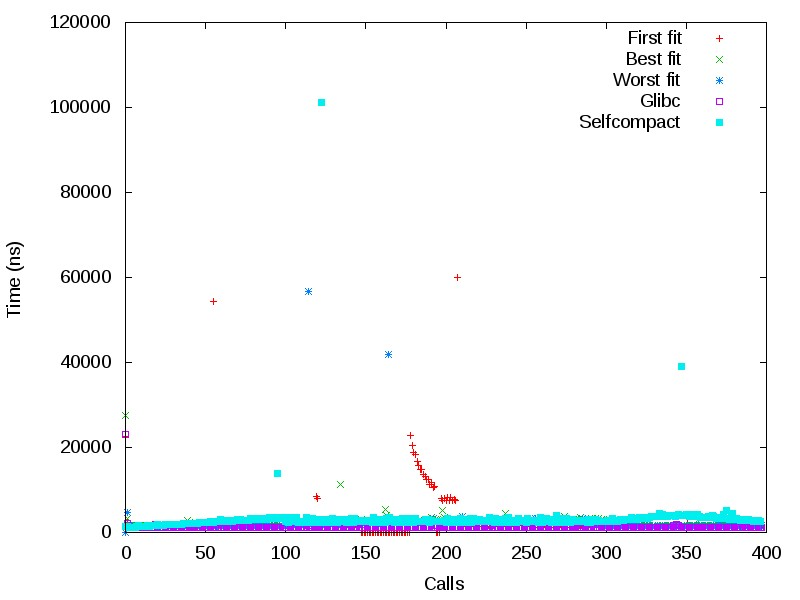
\includegraphics[width=1\linewidth]{Shashkova/images/time_gettime.jpg}}
   \caption{Время выполнения запросов}
   \label{ris:image}
   \end{figure}
   
   Также для различных алгоритмов измерялось время, затраченное аллокаторами на выполнение запросов. На Рис. 5 представлены результаты измерения времени в процессе
   работы программы. Можно заметить, что при некоторых запросах, время в несколько раз превышает среднее время на выделение. Это происходит на запросах о 
   выделении памяти, и, вероятно, это связано с поиском подходящего свободного блока. 
   
   \begin{figure}[p]
   \center{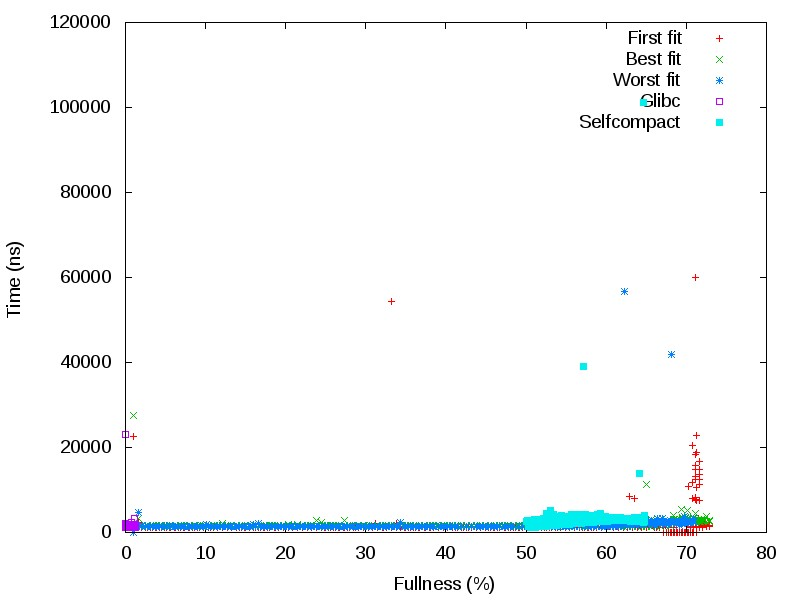
\includegraphics[width=1\linewidth]{Shashkova/images/time_full_self.jpg}}
   \caption{Зависимость времени выполнения запросов от заполненности кучи}
   \label{ris:image}
   \end{figure}
   
   \begin{figure}[p]
   \center{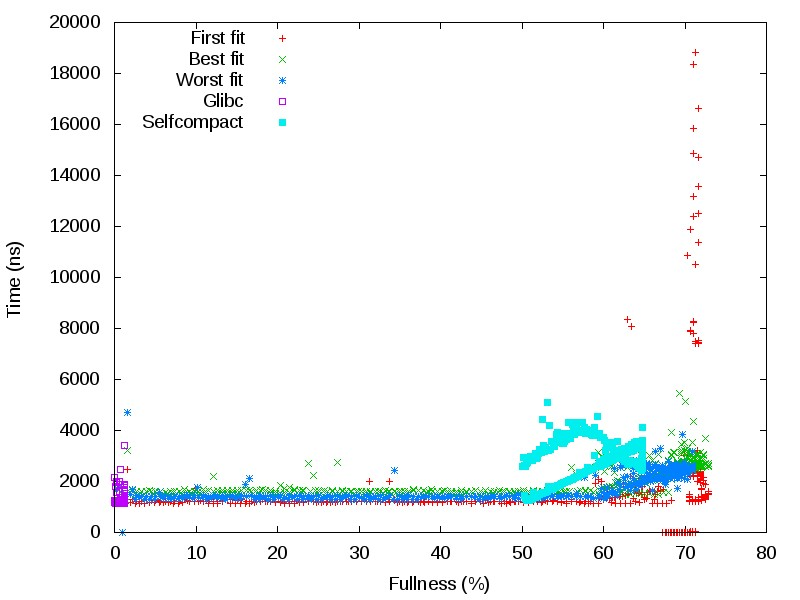
\includegraphics[width=1\linewidth]{Shashkova/images/time_full_zoom_3.jpg}}
   \caption{Зависимость времени выполнения запросов от заполненности кучи, увеличенный масштаб}
   \label{ris:image}
   \end{figure}
   
   На Рис. 6 представлена зависимость времени выделения от заполненности кучи. Наиболее выражена эта зависимость для алгоритма First fit. На Рис. 7 изображена та же
   зависимость с увеличенным масштабом для нижней части графика. На нём видно, что время выполнения запросов у самосжимающейся кучи больше, чем у остальных 
   алгоритмов. Также у всех алгоритмов наблюдается увеличение времени выполнения запросов с приближением заполненности кучи к наибольшему значению.
   
   
   \section{Заключение}
   
   В результате работы над данной курсовой работой:
   
    \begin{itemize}
     \item были изучены существующие метрики для сравнения реализаций кучи;
     \item были изучены подходы для проведения измерений;
     \item была создана система сравнения различных реализаций;
     \item была выявлена ошибка в реализации кучи.
    \end{itemize}

\begin{thebibliography}{99}
\bibitem{six_progs}
Benjamin Zorn, Dirk Grunwald.
Empirical Measurements of Six Allocation-intensive C Programs. University of Colorado, Boulder, 1992.

\bibitem{fragm}
Mark S. Johnstone, Paul R. Wilson.
The Memory Fragmentation Problem: Solved? The University of Texas at Austin, 1997.

\bibitem{un_mutator}
Martin Aigner, Christoph M. Kirsch. Towards a Universal Mutator for Benchmarking Heap Management Systems.
University of Salzburg, 2012.

\bibitem{ae}
James R. Larus. Abstract Execution: a Technique for Efficiently Tracing Programs.
Software --- Practice and Experience.

\bibitem{samofal}
Самофалов А.В. Способы реализации кучи и их свойства // Наст. сборник
\end{thebibliography}

%\documentclass[12pt,a4paper]{article}
%\usepackage[utf8x]{inputenc}
%\usepackage[russian]{babel}
%\usepackage[OT1]{fontenc}
%\usepackage{amsmath}
%\usepackage[a4paper,includeheadfoot,top=20mm,bottom=20mm,left=25mm,right=15mm]{geometry}
%\usepackage{indentfirst}
%\usepackage{amsfonts}
%\usepackage{amssymb}
%\usepackage{graphicx}
%\renewcommand\baselinestretch{1.5}
%\renewcommand\contentsname{Оглавление}

%\begin{document}
%\begin{titlepage}
%\thispagestyle{empty}
%\def\baselinestretch{1.0}
%\begin{center}
%	{\large САНКТ-ПЕТЕРБУРГСКИЙ ГОСУДАРСТВЕННЫЙ УНИВЕРСИТЕТ \\ \vskip 0.3em {\large Математико-механический факультет \\ \vskip 0.7em{\large Кафедра системного программирования \\}}}
%    \vspace*{0.15\textheight}
%    \vfill
%    {\large Шашкова Елизавета Михайловна}
%    
%    \vskip 2em
%    {\huge Методы профилирования реализаций кучи}
%    
%    \vskip 1em
%    {\large Курсовая работа} \\
%    \vskip 2em
%    {\normalsize \raggedleft 
%    Научный руководитель:\\
%    к.ф.-м.н. Д.Ю. Булычев
%    \\[3em]
%    \vspace*{0.08\textheight}
%    \vfill
%    {\centering Санкт-Петербург \\ 2013}
%    }
%\end{center}
%\end{titlepage}

\title{Методы профилирования реализаций кучи}
%
\titlerunning{Методы профилирования реализаций кучи}
\author{Шашкова Елизавета Михайловна}
%
\authorrunning{Е.М.Шашкова} % abbreviated author list (for running head)
%
%%%% list of authors for the TOC (use if author list has to be modified)
\tocauthor{Е.М.Шашкова}
%
\institute{Санк-Петербургский государственный университет\\
\email{Elizaveta239@yandex.ru}}

\maketitle              % typeset the title of the contribution

\begin{abstract}
\end{abstract}
%

\section*{Введение}

   Динамическое управление памятью --- это управление памятью для объектов, ни размер, ни время жизни которых, вообще говоря, неизвестны до
   выполнения программы. Под объектом мы будем понимать некоторый неделимый набор байт.
   
   Обычно при динамическом управлении памятью место под объекты выделяется в специальной области памяти --- \textquotedblleft куче\textquotedblright
   (heap). Существует
   две основных операции для управления памятью в куче: выделение памяти и освобождение. При выделении посылается запрос, в котором указывается количество
   требуемой памяти. При успешном выделении память изымается из кучи, то есть становится недоступна для последующего выделения.
   Освобождение памяти, наоборот, делает часть кучи доступной для последующего выделения.
   
   Поведение динамической памяти удобно описывать в терминах взаимодействия двух основных сущностей: \emph{аллокатора} и \emph{мутатора}. Аллокатор принимает запросы на выделение
   памяти в куче и её освобождение. Мутатор посылает данные запросы. Каждый запрос содержит количество памяти для выделения, причем 
   это количество, вообще говоря, становится известно только в момент исполнения программы.
   
   Эффективность работы программы во многом зависит от эффективности аллокатора. На сегодняшний момент существует много способов его 
   реализации; более того, развитие технологий стимулирует создание новых подходов. Поэтому становится важной задача уметь сравнивать разные
   реализации аллокаторов, находить наиболее подходящие реализации в данном конкретном случае.
   
   Для описания свойств аллокатора можно выделить два полярных подхода:
   \begin{enumerate}
   \item Рассмотрение свойств кучи с точки зрения поведения мутатора. Задача: определить, для какого класса программ данная реализация аллокатора 
   подойдет лучше всего. 
   \item Сравнительный анализ нескольких реализаций аллокатора. Задача: провести сравнение двух или нескольких аллокаторов при взаимодействии с
   одним и тем же мутатором.
   \end{enumerate}
   
   Основные свойства, которыми можно описать аллокатор в первом подходе:
   \begin{itemize}
   \item Суммарное количество выделенной памяти (в байтах и блоках).
   \item Наибольшее количество единовременно выделенной памяти за все время работы программы (в байтах и блоках).
   \item Среднее время жизни блока (в байтах). Это время вычисляется, как количество байт, помещенных в кучу за промежуток времени между 
   созданием и удалением объекта, поделенное на размер объекта (среднее время жизни одного байта в куче).
   \end{itemize}
   
   Основные свойства, которыми можно описать аллокатор во втором подходе:
   \begin{itemize}
   \item Фрагментация. Фрагментация вычисляется по следующей формуле: \[ F = \frac{free - free_{max}}{free} \]
   где $free$ --- количество свободных байт в куче, $free_{max}$ --- размер (в байтах) наибольшего свободного блока.  Так как память в куче выделяется
   блоками (наборами байтов), может так случиться, что в куче не осталось места для блока требуемого размера, хотя количество свободной 
   памяти еще превышает размер этого блока. С помощью данной формулы фрагментацию можно описать численной величиной. Чем меньше эта
   величина, тем \textquotedblleft лучше\textquotedblright~текущее состояние кучи. Фрагментации равна нулю, когда свободное место в 
   куче является одним блоком, и приближается к единице, когда размеры всех свободных блоков в куче малы. 
   \item Время выделения (в единицах времени).
   \item Порог работоспособности (количество запросов, обработанных аллокатором).
   \item Зависимость скорости работы аллокатора от нагрузки.
   \end{itemize}
    
   Цель данной курсовой работы заключается в том, чтобы изучить методы оценки реализации аллокатора. Необходимо понять, насколько 
   эффективно использование того или иного аллокатора, определить критерии, по которым различные аллокаторы будут сравниваться. В 
   соответствии с основными подходами, нужно сравнить поведение одного аллокатора при использовании нескольких различных мутаторов, а также
   сравнить поведение нескольких аллокаторов при работе с одним мутатором. В результате будет создан прототип системы для проведения 
   вышеуказанных сравнений.
   
   
   \section{Существующие подходы и метрики}
   Для сравнения различных реализаций аллокаторов прежде всего нужно выбрать метрики, по которым будет 
   производиться сравнение. Требуется понять, какие данные нужно собирать при запуске программ
   с использованием различных аллокаторов.
   
   В статье ~\cite{six_progs} представлены опытные данные, полученные с помощью шести программ на языке
   C. Авторы запустили каждую программу на нескольких наборах входных данных и построили распределения для следующих величин:
   
   \begin{itemize}
   \item размеров объектов;
   \item времён жизни объектов;
   \item интервалов времени между запросами.
   \end{itemize}
   
   Для этих распределений были найдены среднее, медиана и мода, которые характеризуют асимметричность распределения. Распределение размеров 
   объектов оказалось асимметричным 
   в сторону маленьких размеров: большая часть объектов, под которые выделялась память, имели размер менее 64 байт. Интересным
   оказался тот факт, что 90\% объектов имеют всего 10 различных размеров. Распределение времени жизни
   объектов показало, что большинство объектов живет в течение короткого промежутка времени: 40-80 машинных инструкций процессора 
   
   Данные об использовании памяти были получены посредством трассировки с помощью методики abstract execution~\cite{ae}. В качестве 
   тестовых программ для измерения были взяты: программа, находящая факториал больших целых чисел; оптимизатор Espresso; 
   GhostScript\footnote{http://www.ghostscript.com/} –-- интерпретатор языка PostScript; Gnu Awk\footnote{http://www.gnu.org/software/gawk/} –-- 
   интерпретатор языка AWK; интерпретатор Perl\footnote{http://www.perl.org/}; Chameleon –-- канальный роутер N-го уровня.
   
   Такой способ анализа аллокаторов нельзя полностью отнести ни к первому, ни ко второму подходу, т.к. в программах аллокатор и мутатор
   были фиксированными, изменялись только входные данные. Приоритетом для авторов являлось исследование свойств объектов, для которых выделяется
   память, а не аллокаторов.
   
   В статье ~\cite{fragm} авторы анализировали выделение памяти в нескольких приложениях, чтобы показать, что фрагментацию
   во время исполнения программы можно уменьшить посредством правильного выбора аллокатора. Было показано, что объекты,
   которые помещаются в кучу одновременно, удаляются из неё также одновременно. 
   Параметры, измерявшиеся в процессе работы программ, были таковы:
   
   \begin{itemize}
      \item время работы;
      \item суммарное количество выделенных объектов и байт;
      \item средний размер объектов;
      \item наибольшее количество объектов и байт, одновременно находящихся в куче;
      \item среднее время жизни объектов (в байтах).
   \end{itemize}
   
   Также, как и в предыдущей статье, было показано, что динамические объекты имеют обычно несколько определенных размеров. Был сделан
   вывод, что для уменьшения фрагментации при создании системы выделения памяти нужно опираться прежде всего на данное свойство программ.
   
   В данном исследовании авторы использовали как первый, так и второй подход. Они измеряли фрагментацию по всевозможным комбинациям имеющихся 
   у них мутаторов и аллокаторов.
   
   В ~\cite{un_mutator} авторы описывают созданный ими универсальный мутатор --- ACDC Benchmark Tool. Он представляет собой измеритель, 
   который может эмулировать выделение и очистку памяти и показывать различия между реализациями аллокаторов. Основная идея, заложенная в данном 
   измерителе, заключается в том, чтобы рассматривать в качестве метрики время и измерять его в байтах. Это было сделано для работы не только с
   однопоточными, но и с многопоточными мутаторами. 
   
   С помощью данного инструмента можно осуществить измерения в рамках как первого, так и второго подхода.
   
   
   \section{Проведение измерений}
   В данной работе были реализованы оба подхода к сбору данных. Для первого подхода, который заключается в рассмотрении свойств аллокатора с точки зрения мутатора, измерялись следующие величины:
   \begin{itemize}
      \item суммарное количество выделенной памяти (в байтах и блоках);
      \item наибольшее количество единовременно выделенной памяти за все время работы программы (в байтах и блоках);
      \item среднее время жизни блока (в байтах).
   \end{itemize}
      
   Для второго подхода, основная цель которого --- сравнить аллокаторы с использованием одного мутатора, 
   измерялись:
   \begin{itemize}
         \item фрагментация; 
         \item время выделения (в единицах времени);
         \item порог работоспособности (количество запросов, обработанных аллокатором);
         \item зависимость скорости работы аллокатора от нагрузки.
   \end{itemize}
      
   \subsection{Аллокаторы и мутаторы}
   
   Сбор данных производился как со стандартной реализации аллокатора в glibc, так и с собственной реализации,
   созданной Самофаловым А.В. ~\cite{samofal}. В его работе было реализовано несколько аллокаторов с различными алгоритмами
   выделения памяти.
   
   Эти алгоритмы:
   \begin{itemize}
      \item \textquotedblleft First fit\textquotedblright --- память выделяется в первом свободном блоке;
      \item \textquotedblleft Best fit\textquotedblright --- память выделяется в наиболее подходящем блоке;
      \item \textquotedblleft Worst fit\textquotedblright --- память выделяется в самом большом свободном блоке;
      \item \textquotedblleft Selfcompact\textquotedblright --- cамосжимающаяся куча.
   \end{itemize}
   
   В качестве мутаторов были взяты следующие программы:
   \begin{itemize}
        \item архиватор zip\footnote{http://www.info-zip.org};
   	    \item программа, сортирующая связный список --- sort list;
   	    \item архиватор tar\footnote{http://www.gnu.org/software/tar/}.
   \end{itemize}
   
   \subsection{Подробности реализации}
   
   В стандартной библиотеке языка C существует специальная структура \texttt{mallinfo}, которая описывает состояние кучи. Данная структура имеет следующие поля: 
   \begin{itemize}
   	     \item \texttt{int arena} --- суммарное пространство, выделенное под кучу (в байтах).
         \item \texttt{int ordblks} --- количество свободных блоков.
         \item \texttt{int smblks} --- количество свободных блоков \textquotedblleft fastbin\textquotedblright. Это блоки, которые были освобождены,
         однако, не были объединены с соседними свободными блоками. В этих блоках впоследствии можно 
         выделять память под объекты такого же размера.
          \item \texttt{int hblks} --- суммарное количество блоков, находящихся в куче.
          \item \texttt{int hblkhd} --- суммарное место, выделенное под блоки (в байтах).
          \item \texttt{int usmblks} --- наибольшее количество байт, находящихся в куче за время работы программы.
          \item \texttt{int fsmblks} --- суммарное место в блоках \textquotedblleft fastbin\textquotedblright (в байтах).
          \item \texttt{int uordblks} --- суммарное занятое пространство (в байтах).
          \item \texttt{int fordblks} --- суммарное свободное пространство (в байтах).
          \item \texttt{int keepcost} --- наибольшее количество пространства, которое можно освободить в начале кучи 
          (то есть посредством функции \texttt{malloc\_trim}) (в байтах).
   \end{itemize}
   
   Функция \texttt{mallinfo} возвращает копию структуры \texttt{mallinfo}. С её помощью были измерены некоторые величины для стандартной реализации аллокатора. 
   Для осуществления измерений были использованы hook-функции. Переменные \texttt{\_\_malloc\_hook}, \texttt{\_\_realloc\_hook} и \texttt{\_\_free\_hook} являются 
   указателями на функции, которые используют функции \texttt{malloc}, \texttt{realloc} и \texttt{free} соответственно всякий раз, когда они вызываются. Таким 
   образом можно привязывать вызов требуемых функций (в нашем случае --- сбор статистики) к запросам на выделение или очистку памяти.
   
   В собственной реализации для сбора статистики был создан аналог структуры \texttt{mallinfo} --- структура \texttt{myinfo}.
   Её устройство схоже с устройством \texttt{mallinfo}, однако, имеются некоторые различия. Она содержит следующие поля:
   \begin{itemize}
     \item \texttt{int arena} --- суммарное пространство, выделенное под кучу (в байтах);
     \item \texttt{int freemem} --- свободное пространство (в байтах);
     \item \texttt{int usdmem} --- занятое пространство (в байтах);
     \item \texttt{int freeblks} --- количество свободных блоков;
     \item \texttt{nt usdblks} --- количество используемых блоков;
     \item \texttt{maxfreeblk} --- размер наибольшего свободного блока (в байтах).
   \end{itemize} 
   
   Основным отличием данной структуры от структуры \texttt{mallinfo} является наличие поля с размером наибольшего свободного
   блока. Оно позволяет напрямую использовать это значение для вычисления фрагментации (по формуле, упоминавшейся
   во введении).
   
   
   \section{Результаты}
   
   Результаты измерений в первом подходе --- данные, усредненные по выполнению программы. Результаты представлены в следующих таблицах. Max(bytes) обозначает
   наибольшее количество единовременно выделенной памяти(в байтах). Sum(bytes) обозначает общее количество выделенной памяти(в байтах). Mean lifetime(bytes)
   обозначает среднее время жизни блока(в байтах).
    
    First fit:
    \begin{center}
    \begin{tabular}{| l | c | c | c | c | c |}
    \hline
    Мутатор & Max(bytes) & Max(blocks) & Sum(bytes) & Sum(blocks) & Mean lifetime(bytes)\\
    \hline
    zip & 21064 & 53 & 25845 & 77 & 1068.48\\
    \hline
    sort list & 808 & 101 & 1592 & 199 & 82.21 \\
    \hline
    tar & 52080 & 238 & 58736 & 404 & 446.86 \\
    \hline
    \end{tabular}
    \end{center}

    Best fit:
    \begin{center}
    \begin{tabular}{| l | c | c | c | c | c |}
    \hline
    Мутатор & Max(bytes) & Max(blocks) & Sum(bytes) & Sum(blocks) & Mean lifetime(bytes)\\
    \hline
    zip & 21080 & 53 & 25845 & 75 & 1068.64\\
    \hline
    sort list & 808 & 101 & 1592 & 199 & 82.27 \\
    \hline
    tar & 52112 & 238 & 58736 & 402 & 451.89 \\
    \hline
    \end{tabular}
    \end{center}
    
    Worst fit:
    \begin{center}
    \begin{tabular}{| l | c | c | c | c | c |}
    \hline
    Мутатор & Max(bytes) & Max(blocks) & Sum(bytes) & Sum(blocks) & Mean lifetime(bytes)\\
    \hline
    zip & 21064 & 53 & 25845 & 80 & 1069.85\\
    \hline
    sort list & 808 & 101 & 1592 & 199 & 80.72\\
    \hline
    tar & 52080 & 238 & 58736 & 404 & 455.58 \\
    \hline
    \end{tabular}
    \end{center}
    
   Средние величины для всех аллокаторов получились почти одинаковые. Данный подход к изучению аллокаторов не выявил их различий и особенностей.
    
   
   Во втором подходе измерения и сравнения производились после каждого запроса, которыми обменивались между собой аллокатор и мутатор. В связи с этим,
   полученные данные удобно представить в виде графиков.
   
   На Рис. 1 представлено изменение фрагментации для алгоритмов First fit, Best fit и Worst fit при работе с программой zip. Из пяти возможных аллокаторов
   величину фрагментации с мутатором zip удалось найти только для данных трех. Это связано с тем, что для стандартной реализации аллокатора фрагментацию по нашей
   формуле найти не удастся, так как нет возможности узнать размер наибольшего свободного блока. А аллокатор selfcompact требует специфичного написания мутатора и 
   его компиляции, поэтому запустить этот аллокатор с мутатором zip не представляется возможным.
   
   \begin{figure}[h]
   \center{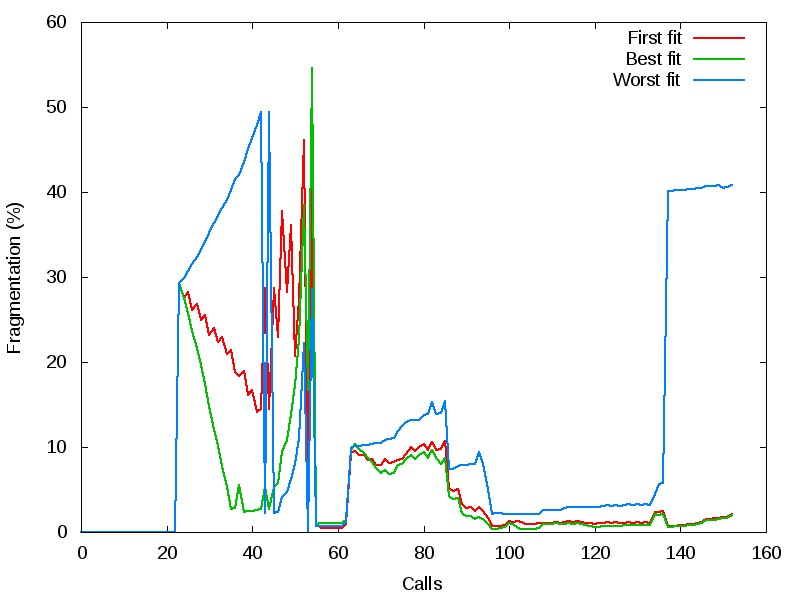
\includegraphics[width=1\linewidth]{Shashkova/images/fragment_zip.jpg}}
   \caption{Величина фрагментации с мутатором zip}
   \label{ris:image}
   \end{figure}
   
   Можно заметить, что первом участке у всех трех аллокаторов величина фрагментации равна 0. Это связано с тем, что освобождения памяти еще не производились и объекты
   находятся в куче последовательно, без пропусков. Затем фрагментация начинает возрастать. Как и предполагалось теоретически, почти на всех участках графика 
   фрагментация аллокатора Worst fit больше фрагментации остальных аллокаторов, а фрагментация аллокатора Best fit меньше фрагментации остальных аллокаторов.
   
   \begin{figure}[p]
   \center{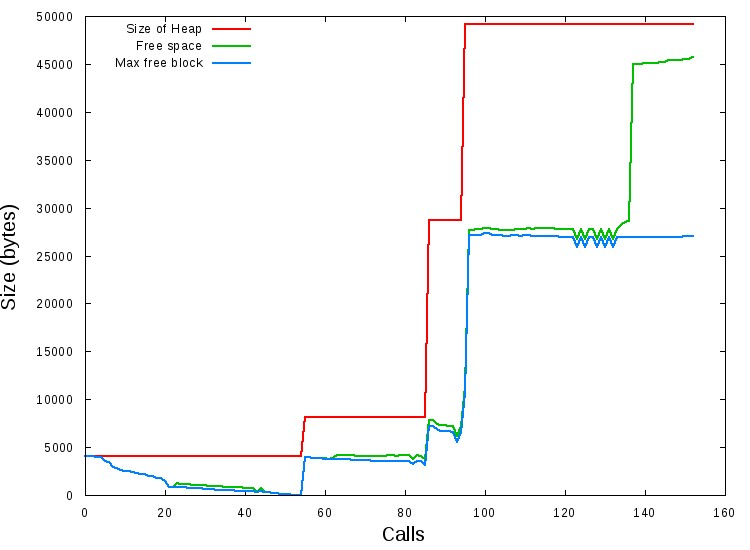
\includegraphics[width=1\linewidth]{Shashkova/images/size_zip_worst.jpg}}
   \caption{Состояние кучи с аллокаторм Worst fit и мутатором zip}
   \label{ris:image}
   \end{figure}
   
   Можно отметить резкий скачок, а затем резкое уменьшение фрагментации в районе 60-го запроса. Для объяснения такого поведения, рассмотрим график размера кучи, 
   например, для аллокатора Worst fit(см. Рис. 2). На нем представлены размер кучи, размер свободного пространства в куче и величина максимального свободного
   блока.
   Тогда становится понятным, что резкое изменение фрагментации в районе 60-го запроса связано с увеличением размера кучи (добавляется большой свободный блок). 
   Подобное повторяется в районе 82-го и 98-го запросов, однако, там фрагментация изменяется не столь резко. Это связано с тем, что общий размер кучи к тому моменту
   уже значительно увеличился.
   
   
   \begin{figure}[p]
   \center{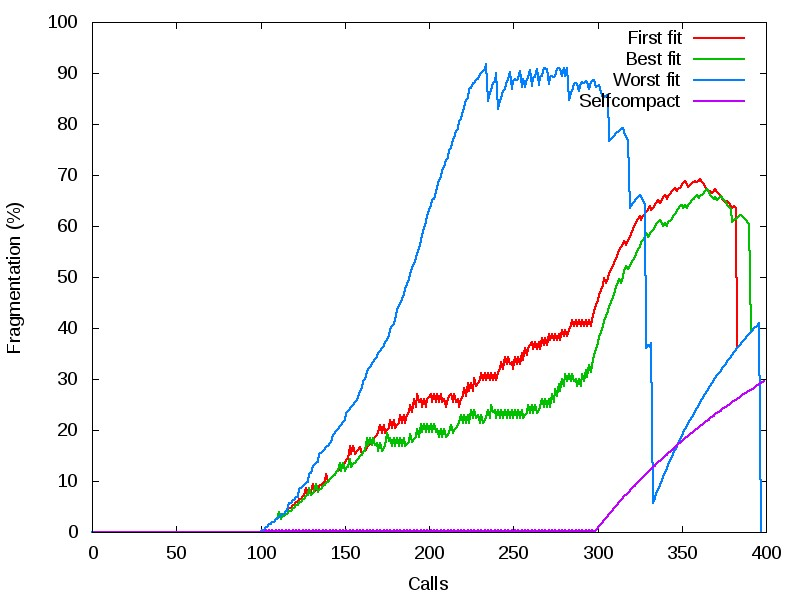
\includegraphics[width=1\linewidth]{Shashkova/images/fragment_list_selfcomp.jpg}}
   \caption{Величина фрагментации с мутатором sort list}
   \label{ris:image}
   \end{figure}
   
   На Рис. 3 представлена величина фрагментации в процессе исполнения программы --- сортировки связного списка --- для четырех аллокаторов. На первом участке графика
   видно, что для всех аллокатором величина фрагментации равна 0. На этом участке список создается, объекты располагаются в куче последовательно и все свободное
   пространство является одним блоком. 
   
   Затем, в процессе сортировки, некоторые объекты удаляются, под новые выделяется память. Здесь сразу можно заметить, что фрагментация алгоритма Worst fit растет
   быстрее фрагментации других алгоритмов. Около 300-го запроса можно отметить увеличение фрагментации у алгоритмов First fit и Best fit. 
   
   \begin{figure}[p]
   \center{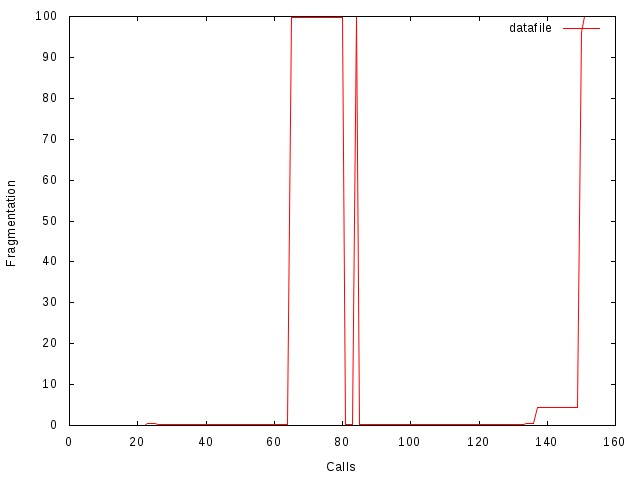
\includegraphics[width=1\linewidth]{Shashkova/images/fragment_bad.jpg}}
   \caption{Величина фрагментации аллокатора First fit}
   \label{ris:image}
   \end{figure}
   
    Хочется отметить, что сбор статистики помог выявить ошибку в первоначальной реализации аллокатора First fit. На Рис. 4 представлено, как изменялась фрагментация
   на одной из первых тестовых программ. 
   Такое резкое изменение фрагментации показалось нам неестественным. Благодаря этому была проведена перепроверка реализации и 
   выявлена ошибка.
   
   \begin{figure}[p]
   \center{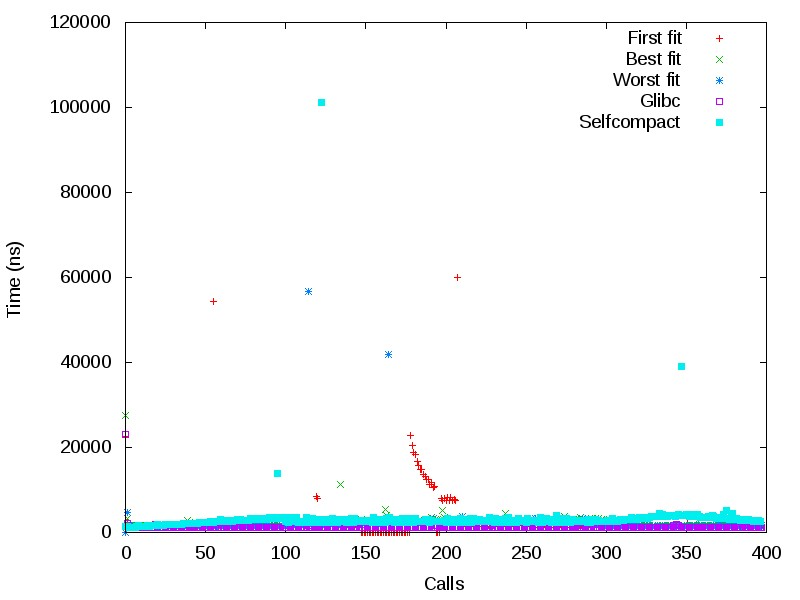
\includegraphics[width=1\linewidth]{Shashkova/images/time_gettime.jpg}}
   \caption{Время выполнения запросов}
   \label{ris:image}
   \end{figure}
   
   Также для различных алгоритмов измерялось время, затраченное аллокаторами на выполнение запросов. На Рис. 5 представлены результаты измерения времени в процессе
   работы программы. Можно заметить, что при некоторых запросах, время в несколько раз превышает среднее время на выделение. Это происходит на запросах о 
   выделении памяти, и, вероятно, это связано с поиском подходящего свободного блока. 
   
   \begin{figure}[p]
   \center{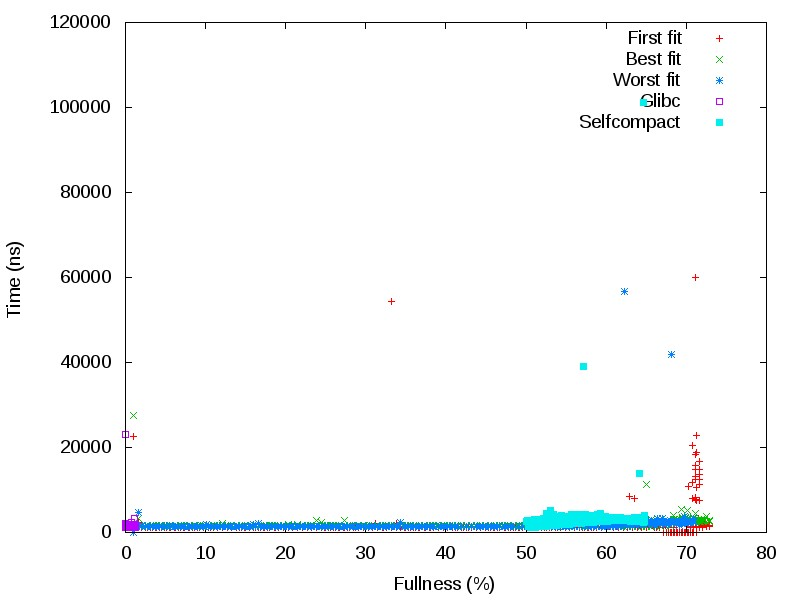
\includegraphics[width=1\linewidth]{Shashkova/images/time_full_self.jpg}}
   \caption{Зависимость времени выполнения запросов от заполненности кучи}
   \label{ris:image}
   \end{figure}
   
   \begin{figure}[p]
   \center{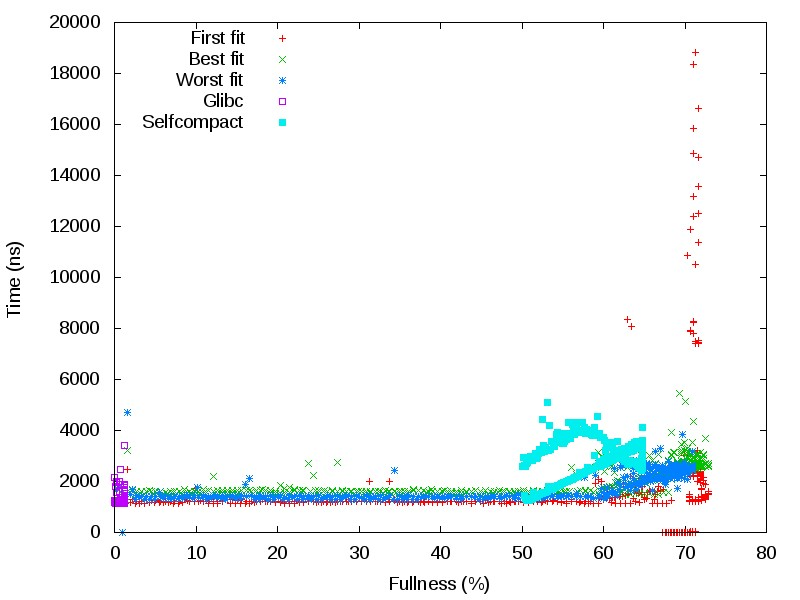
\includegraphics[width=1\linewidth]{Shashkova/images/time_full_zoom_3.jpg}}
   \caption{Зависимость времени выполнения запросов от заполненности кучи, увеличенный масштаб}
   \label{ris:image}
   \end{figure}
   
   На Рис. 6 представлена зависимость времени выделения от заполненности кучи. Наиболее выражена эта зависимость для алгоритма First fit. На Рис. 7 изображена та же
   зависимость с увеличенным масштабом для нижней части графика. На нём видно, что время выполнения запросов у самосжимающейся кучи больше, чем у остальных 
   алгоритмов. Также у всех алгоритмов наблюдается увеличение времени выполнения запросов с приближением заполненности кучи к наибольшему значению.
   
   
   \section{Заключение}
   
   В результате работы над данной курсовой работой:
   
    \begin{itemize}
     \item были изучены существующие метрики для сравнения реализаций кучи;
     \item были изучены подходы для проведения измерений;
     \item была создана система сравнения различных реализаций;
     \item была выявлена ошибка в реализации кучи.
    \end{itemize}

\begin{thebibliography}{99}
\bibitem{six_progs}
Benjamin Zorn, Dirk Grunwald.
Empirical Measurements of Six Allocation-intensive C Programs. University of Colorado, Boulder, 1992.

\bibitem{fragm}
Mark S. Johnstone, Paul R. Wilson.
The Memory Fragmentation Problem: Solved? The University of Texas at Austin, 1997.

\bibitem{un_mutator}
Martin Aigner, Christoph M. Kirsch. Towards a Universal Mutator for Benchmarking Heap Management Systems.
University of Salzburg, 2012.

\bibitem{ae}
James R. Larus. Abstract Execution: a Technique for Efficiently Tracing Programs.
Software --- Practice and Experience.

\bibitem{samofal}
Самофалов А.В. Способы реализации кучи и их свойства // Наст. сборник
\end{thebibliography}


%\documentclass[12pt,a4paper]{article}
%\usepackage[utf8x]{inputenc}
%\usepackage[russian]{babel}
%\usepackage[OT1]{fontenc}
%\usepackage{amsmath}
%\usepackage[a4paper,includeheadfoot,top=20mm,bottom=20mm,left=25mm,right=15mm]{geometry}
%\usepackage{indentfirst}
%\usepackage{amsfonts}
%\usepackage{amssymb}
%\usepackage{graphicx}
%\renewcommand\baselinestretch{1.5}
%\renewcommand\contentsname{Оглавление}

%\begin{document}
%\begin{titlepage}
%\thispagestyle{empty}
%\def\baselinestretch{1.0}
%\begin{center}
%	{\large САНКТ-ПЕТЕРБУРГСКИЙ ГОСУДАРСТВЕННЫЙ УНИВЕРСИТЕТ \\ \vskip 0.3em {\large Математико-механический факультет \\ \vskip 0.7em{\large Кафедра системного программирования \\}}}
%    \vspace*{0.15\textheight}
%    \vfill
%    {\large Шашкова Елизавета Михайловна}
%    
%    \vskip 2em
%    {\huge Методы профилирования реализаций кучи}
%    
%    \vskip 1em
%    {\large Курсовая работа} \\
%    \vskip 2em
%    {\normalsize \raggedleft 
%    Научный руководитель:\\
%    к.ф.-м.н. Д.Ю. Булычев
%    \\[3em]
%    \vspace*{0.08\textheight}
%    \vfill
%    {\centering Санкт-Петербург \\ 2013}
%    }
%\end{center}
%\end{titlepage}

\title{Методы профилирования реализаций кучи}
%
\titlerunning{Методы профилирования реализаций кучи}
\author{Шашкова Елизавета Михайловна}
%
\authorrunning{Е.М.Шашкова} % abbreviated author list (for running head)
%
%%%% list of authors for the TOC (use if author list has to be modified)
\tocauthor{Е.М.Шашкова}
%
\institute{Санк-Петербургский государственный университет\\
\email{Elizaveta239@yandex.ru}}

\maketitle              % typeset the title of the contribution

\begin{abstract}
\end{abstract}
%

\section*{Введение}

   Динамическое управление памятью --- это управление памятью для объектов, ни размер, ни время жизни которых, вообще говоря, неизвестны до
   выполнения программы. Под объектом мы будем понимать некоторый неделимый набор байт.
   
   Обычно при динамическом управлении памятью место под объекты выделяется в специальной области памяти --- \textquotedblleft куче\textquotedblright
   (heap). Существует
   две основных операции для управления памятью в куче: выделение памяти и освобождение. При выделении посылается запрос, в котором указывается количество
   требуемой памяти. При успешном выделении память изымается из кучи, то есть становится недоступна для последующего выделения.
   Освобождение памяти, наоборот, делает часть кучи доступной для последующего выделения.
   
   Поведение динамической памяти удобно описывать в терминах взаимодействия двух основных сущностей: \emph{аллокатора} и \emph{мутатора}. Аллокатор принимает запросы на выделение
   памяти в куче и её освобождение. Мутатор посылает данные запросы. Каждый запрос содержит количество памяти для выделения, причем 
   это количество, вообще говоря, становится известно только в момент исполнения программы.
   
   Эффективность работы программы во многом зависит от эффективности аллокатора. На сегодняшний момент существует много способов его 
   реализации; более того, развитие технологий стимулирует создание новых подходов. Поэтому становится важной задача уметь сравнивать разные
   реализации аллокаторов, находить наиболее подходящие реализации в данном конкретном случае.
   
   Для описания свойств аллокатора можно выделить два полярных подхода:
   \begin{enumerate}
   \item Рассмотрение свойств кучи с точки зрения поведения мутатора. Задача: определить, для какого класса программ данная реализация аллокатора 
   подойдет лучше всего. 
   \item Сравнительный анализ нескольких реализаций аллокатора. Задача: провести сравнение двух или нескольких аллокаторов при взаимодействии с
   одним и тем же мутатором.
   \end{enumerate}
   
   Основные свойства, которыми можно описать аллокатор в первом подходе:
   \begin{itemize}
   \item Суммарное количество выделенной памяти (в байтах и блоках).
   \item Наибольшее количество единовременно выделенной памяти за все время работы программы (в байтах и блоках).
   \item Среднее время жизни блока (в байтах). Это время вычисляется, как количество байт, помещенных в кучу за промежуток времени между 
   созданием и удалением объекта, поделенное на размер объекта (среднее время жизни одного байта в куче).
   \end{itemize}
   
   Основные свойства, которыми можно описать аллокатор во втором подходе:
   \begin{itemize}
   \item Фрагментация. Фрагментация вычисляется по следующей формуле: \[ F = \frac{free - free_{max}}{free} \]
   где $free$ --- количество свободных байт в куче, $free_{max}$ --- размер (в байтах) наибольшего свободного блока.  Так как память в куче выделяется
   блоками (наборами байтов), может так случиться, что в куче не осталось места для блока требуемого размера, хотя количество свободной 
   памяти еще превышает размер этого блока. С помощью данной формулы фрагментацию можно описать численной величиной. Чем меньше эта
   величина, тем \textquotedblleft лучше\textquotedblright~текущее состояние кучи. Фрагментации равна нулю, когда свободное место в 
   куче является одним блоком, и приближается к единице, когда размеры всех свободных блоков в куче малы. 
   \item Время выделения (в единицах времени).
   \item Порог работоспособности (количество запросов, обработанных аллокатором).
   \item Зависимость скорости работы аллокатора от нагрузки.
   \end{itemize}
    
   Цель данной курсовой работы заключается в том, чтобы изучить методы оценки реализации аллокатора. Необходимо понять, насколько 
   эффективно использование того или иного аллокатора, определить критерии, по которым различные аллокаторы будут сравниваться. В 
   соответствии с основными подходами, нужно сравнить поведение одного аллокатора при использовании нескольких различных мутаторов, а также
   сравнить поведение нескольких аллокаторов при работе с одним мутатором. В результате будет создан прототип системы для проведения 
   вышеуказанных сравнений.
   
   
   \section{Существующие подходы и метрики}
   Для сравнения различных реализаций аллокаторов прежде всего нужно выбрать метрики, по которым будет 
   производиться сравнение. Требуется понять, какие данные нужно собирать при запуске программ
   с использованием различных аллокаторов.
   
   В статье ~\cite{six_progs} представлены опытные данные, полученные с помощью шести программ на языке
   C. Авторы запустили каждую программу на нескольких наборах входных данных и построили распределения для следующих величин:
   
   \begin{itemize}
   \item размеров объектов;
   \item времён жизни объектов;
   \item интервалов времени между запросами.
   \end{itemize}
   
   Для этих распределений были найдены среднее, медиана и мода, которые характеризуют асимметричность распределения. Распределение размеров 
   объектов оказалось асимметричным 
   в сторону маленьких размеров: большая часть объектов, под которые выделялась память, имели размер менее 64 байт. Интересным
   оказался тот факт, что 90\% объектов имеют всего 10 различных размеров. Распределение времени жизни
   объектов показало, что большинство объектов живет в течение короткого промежутка времени: 40-80 машинных инструкций процессора 
   
   Данные об использовании памяти были получены посредством трассировки с помощью методики abstract execution~\cite{ae}. В качестве 
   тестовых программ для измерения были взяты: программа, находящая факториал больших целых чисел; оптимизатор Espresso; 
   GhostScript\footnote{http://www.ghostscript.com/} –-- интерпретатор языка PostScript; Gnu Awk\footnote{http://www.gnu.org/software/gawk/} –-- 
   интерпретатор языка AWK; интерпретатор Perl\footnote{http://www.perl.org/}; Chameleon –-- канальный роутер N-го уровня.
   
   Такой способ анализа аллокаторов нельзя полностью отнести ни к первому, ни ко второму подходу, т.к. в программах аллокатор и мутатор
   были фиксированными, изменялись только входные данные. Приоритетом для авторов являлось исследование свойств объектов, для которых выделяется
   память, а не аллокаторов.
   
   В статье ~\cite{fragm} авторы анализировали выделение памяти в нескольких приложениях, чтобы показать, что фрагментацию
   во время исполнения программы можно уменьшить посредством правильного выбора аллокатора. Было показано, что объекты,
   которые помещаются в кучу одновременно, удаляются из неё также одновременно. 
   Параметры, измерявшиеся в процессе работы программ, были таковы:
   
   \begin{itemize}
      \item время работы;
      \item суммарное количество выделенных объектов и байт;
      \item средний размер объектов;
      \item наибольшее количество объектов и байт, одновременно находящихся в куче;
      \item среднее время жизни объектов (в байтах).
   \end{itemize}
   
   Также, как и в предыдущей статье, было показано, что динамические объекты имеют обычно несколько определенных размеров. Был сделан
   вывод, что для уменьшения фрагментации при создании системы выделения памяти нужно опираться прежде всего на данное свойство программ.
   
   В данном исследовании авторы использовали как первый, так и второй подход. Они измеряли фрагментацию по всевозможным комбинациям имеющихся 
   у них мутаторов и аллокаторов.
   
   В ~\cite{un_mutator} авторы описывают созданный ими универсальный мутатор --- ACDC Benchmark Tool. Он представляет собой измеритель, 
   который может эмулировать выделение и очистку памяти и показывать различия между реализациями аллокаторов. Основная идея, заложенная в данном 
   измерителе, заключается в том, чтобы рассматривать в качестве метрики время и измерять его в байтах. Это было сделано для работы не только с
   однопоточными, но и с многопоточными мутаторами. 
   
   С помощью данного инструмента можно осуществить измерения в рамках как первого, так и второго подхода.
   
   
   \section{Проведение измерений}
   В данной работе были реализованы оба подхода к сбору данных. Для первого подхода, который заключается в рассмотрении свойств аллокатора с точки зрения мутатора, измерялись следующие величины:
   \begin{itemize}
      \item суммарное количество выделенной памяти (в байтах и блоках);
      \item наибольшее количество единовременно выделенной памяти за все время работы программы (в байтах и блоках);
      \item среднее время жизни блока (в байтах).
   \end{itemize}
      
   Для второго подхода, основная цель которого --- сравнить аллокаторы с использованием одного мутатора, 
   измерялись:
   \begin{itemize}
         \item фрагментация; 
         \item время выделения (в единицах времени);
         \item порог работоспособности (количество запросов, обработанных аллокатором);
         \item зависимость скорости работы аллокатора от нагрузки.
   \end{itemize}
      
   \subsection{Аллокаторы и мутаторы}
   
   Сбор данных производился как со стандартной реализации аллокатора в glibc, так и с собственной реализации,
   созданной Самофаловым А.В. ~\cite{samofal}. В его работе было реализовано несколько аллокаторов с различными алгоритмами
   выделения памяти.
   
   Эти алгоритмы:
   \begin{itemize}
      \item \textquotedblleft First fit\textquotedblright --- память выделяется в первом свободном блоке;
      \item \textquotedblleft Best fit\textquotedblright --- память выделяется в наиболее подходящем блоке;
      \item \textquotedblleft Worst fit\textquotedblright --- память выделяется в самом большом свободном блоке;
      \item \textquotedblleft Selfcompact\textquotedblright --- cамосжимающаяся куча.
   \end{itemize}
   
   В качестве мутаторов были взяты следующие программы:
   \begin{itemize}
        \item архиватор zip\footnote{http://www.info-zip.org};
   	    \item программа, сортирующая связный список --- sort list;
   	    \item архиватор tar\footnote{http://www.gnu.org/software/tar/}.
   \end{itemize}
   
   \subsection{Подробности реализации}
   
   В стандартной библиотеке языка C существует специальная структура \texttt{mallinfo}, которая описывает состояние кучи. Данная структура имеет следующие поля: 
   \begin{itemize}
   	     \item \texttt{int arena} --- суммарное пространство, выделенное под кучу (в байтах).
         \item \texttt{int ordblks} --- количество свободных блоков.
         \item \texttt{int smblks} --- количество свободных блоков \textquotedblleft fastbin\textquotedblright. Это блоки, которые были освобождены,
         однако, не были объединены с соседними свободными блоками. В этих блоках впоследствии можно 
         выделять память под объекты такого же размера.
          \item \texttt{int hblks} --- суммарное количество блоков, находящихся в куче.
          \item \texttt{int hblkhd} --- суммарное место, выделенное под блоки (в байтах).
          \item \texttt{int usmblks} --- наибольшее количество байт, находящихся в куче за время работы программы.
          \item \texttt{int fsmblks} --- суммарное место в блоках \textquotedblleft fastbin\textquotedblright (в байтах).
          \item \texttt{int uordblks} --- суммарное занятое пространство (в байтах).
          \item \texttt{int fordblks} --- суммарное свободное пространство (в байтах).
          \item \texttt{int keepcost} --- наибольшее количество пространства, которое можно освободить в начале кучи 
          (то есть посредством функции \texttt{malloc\_trim}) (в байтах).
   \end{itemize}
   
   Функция \texttt{mallinfo} возвращает копию структуры \texttt{mallinfo}. С её помощью были измерены некоторые величины для стандартной реализации аллокатора. 
   Для осуществления измерений были использованы hook-функции. Переменные \texttt{\_\_malloc\_hook}, \texttt{\_\_realloc\_hook} и \texttt{\_\_free\_hook} являются 
   указателями на функции, которые используют функции \texttt{malloc}, \texttt{realloc} и \texttt{free} соответственно всякий раз, когда они вызываются. Таким 
   образом можно привязывать вызов требуемых функций (в нашем случае --- сбор статистики) к запросам на выделение или очистку памяти.
   
   В собственной реализации для сбора статистики был создан аналог структуры \texttt{mallinfo} --- структура \texttt{myinfo}.
   Её устройство схоже с устройством \texttt{mallinfo}, однако, имеются некоторые различия. Она содержит следующие поля:
   \begin{itemize}
     \item \texttt{int arena} --- суммарное пространство, выделенное под кучу (в байтах);
     \item \texttt{int freemem} --- свободное пространство (в байтах);
     \item \texttt{int usdmem} --- занятое пространство (в байтах);
     \item \texttt{int freeblks} --- количество свободных блоков;
     \item \texttt{nt usdblks} --- количество используемых блоков;
     \item \texttt{maxfreeblk} --- размер наибольшего свободного блока (в байтах).
   \end{itemize} 
   
   Основным отличием данной структуры от структуры \texttt{mallinfo} является наличие поля с размером наибольшего свободного
   блока. Оно позволяет напрямую использовать это значение для вычисления фрагментации (по формуле, упоминавшейся
   во введении).
   
   
   \section{Результаты}
   
   Результаты измерений в первом подходе --- данные, усредненные по выполнению программы. Результаты представлены в следующих таблицах. Max(bytes) обозначает
   наибольшее количество единовременно выделенной памяти(в байтах). Sum(bytes) обозначает общее количество выделенной памяти(в байтах). Mean lifetime(bytes)
   обозначает среднее время жизни блока(в байтах).
    
    First fit:
    \begin{center}
    \begin{tabular}{| l | c | c | c | c | c |}
    \hline
    Мутатор & Max(bytes) & Max(blocks) & Sum(bytes) & Sum(blocks) & Mean lifetime(bytes)\\
    \hline
    zip & 21064 & 53 & 25845 & 77 & 1068.48\\
    \hline
    sort list & 808 & 101 & 1592 & 199 & 82.21 \\
    \hline
    tar & 52080 & 238 & 58736 & 404 & 446.86 \\
    \hline
    \end{tabular}
    \end{center}

    Best fit:
    \begin{center}
    \begin{tabular}{| l | c | c | c | c | c |}
    \hline
    Мутатор & Max(bytes) & Max(blocks) & Sum(bytes) & Sum(blocks) & Mean lifetime(bytes)\\
    \hline
    zip & 21080 & 53 & 25845 & 75 & 1068.64\\
    \hline
    sort list & 808 & 101 & 1592 & 199 & 82.27 \\
    \hline
    tar & 52112 & 238 & 58736 & 402 & 451.89 \\
    \hline
    \end{tabular}
    \end{center}
    
    Worst fit:
    \begin{center}
    \begin{tabular}{| l | c | c | c | c | c |}
    \hline
    Мутатор & Max(bytes) & Max(blocks) & Sum(bytes) & Sum(blocks) & Mean lifetime(bytes)\\
    \hline
    zip & 21064 & 53 & 25845 & 80 & 1069.85\\
    \hline
    sort list & 808 & 101 & 1592 & 199 & 80.72\\
    \hline
    tar & 52080 & 238 & 58736 & 404 & 455.58 \\
    \hline
    \end{tabular}
    \end{center}
    
   Средние величины для всех аллокаторов получились почти одинаковые. Данный подход к изучению аллокаторов не выявил их различий и особенностей.
    
   
   Во втором подходе измерения и сравнения производились после каждого запроса, которыми обменивались между собой аллокатор и мутатор. В связи с этим,
   полученные данные удобно представить в виде графиков.
   
   На Рис. 1 представлено изменение фрагментации для алгоритмов First fit, Best fit и Worst fit при работе с программой zip. Из пяти возможных аллокаторов
   величину фрагментации с мутатором zip удалось найти только для данных трех. Это связано с тем, что для стандартной реализации аллокатора фрагментацию по нашей
   формуле найти не удастся, так как нет возможности узнать размер наибольшего свободного блока. А аллокатор selfcompact требует специфичного написания мутатора и 
   его компиляции, поэтому запустить этот аллокатор с мутатором zip не представляется возможным.
   
   \begin{figure}[h]
   \center{\includegraphics[width=1\linewidth]{Shashkova/images/fragment_zip.jpg}}
   \caption{Величина фрагментации с мутатором zip}
   \label{ris:image}
   \end{figure}
   
   Можно заметить, что первом участке у всех трех аллокаторов величина фрагментации равна 0. Это связано с тем, что освобождения памяти еще не производились и объекты
   находятся в куче последовательно, без пропусков. Затем фрагментация начинает возрастать. Как и предполагалось теоретически, почти на всех участках графика 
   фрагментация аллокатора Worst fit больше фрагментации остальных аллокаторов, а фрагментация аллокатора Best fit меньше фрагментации остальных аллокаторов.
   
   \begin{figure}[p]
   \center{\includegraphics[width=1\linewidth]{Shashkova/images/size_zip_worst.jpg}}
   \caption{Состояние кучи с аллокаторм Worst fit и мутатором zip}
   \label{ris:image}
   \end{figure}
   
   Можно отметить резкий скачок, а затем резкое уменьшение фрагментации в районе 60-го запроса. Для объяснения такого поведения, рассмотрим график размера кучи, 
   например, для аллокатора Worst fit(см. Рис. 2). На нем представлены размер кучи, размер свободного пространства в куче и величина максимального свободного
   блока.
   Тогда становится понятным, что резкое изменение фрагментации в районе 60-го запроса связано с увеличением размера кучи (добавляется большой свободный блок). 
   Подобное повторяется в районе 82-го и 98-го запросов, однако, там фрагментация изменяется не столь резко. Это связано с тем, что общий размер кучи к тому моменту
   уже значительно увеличился.
   
   
   \begin{figure}[p]
   \center{\includegraphics[width=1\linewidth]{Shashkova/images/fragment_list_selfcomp.jpg}}
   \caption{Величина фрагментации с мутатором sort list}
   \label{ris:image}
   \end{figure}
   
   На Рис. 3 представлена величина фрагментации в процессе исполнения программы --- сортировки связного списка --- для четырех аллокаторов. На первом участке графика
   видно, что для всех аллокатором величина фрагментации равна 0. На этом участке список создается, объекты располагаются в куче последовательно и все свободное
   пространство является одним блоком. 
   
   Затем, в процессе сортировки, некоторые объекты удаляются, под новые выделяется память. Здесь сразу можно заметить, что фрагментация алгоритма Worst fit растет
   быстрее фрагментации других алгоритмов. Около 300-го запроса можно отметить увеличение фрагментации у алгоритмов First fit и Best fit. 
   
   \begin{figure}[p]
   \center{\includegraphics[width=1\linewidth]{Shashkova/images/fragment_bad.jpg}}
   \caption{Величина фрагментации аллокатора First fit}
   \label{ris:image}
   \end{figure}
   
    Хочется отметить, что сбор статистики помог выявить ошибку в первоначальной реализации аллокатора First fit. На Рис. 4 представлено, как изменялась фрагментация
   на одной из первых тестовых программ. 
   Такое резкое изменение фрагментации показалось нам неестественным. Благодаря этому была проведена перепроверка реализации и 
   выявлена ошибка.
   
   \begin{figure}[p]
   \center{\includegraphics[width=1\linewidth]{Shashkova/images/time_gettime.jpg}}
   \caption{Время выполнения запросов}
   \label{ris:image}
   \end{figure}
   
   Также для различных алгоритмов измерялось время, затраченное аллокаторами на выполнение запросов. На Рис. 5 представлены результаты измерения времени в процессе
   работы программы. Можно заметить, что при некоторых запросах, время в несколько раз превышает среднее время на выделение. Это происходит на запросах о 
   выделении памяти, и, вероятно, это связано с поиском подходящего свободного блока. 
   
   \begin{figure}[p]
   \center{\includegraphics[width=1\linewidth]{Shashkova/images/time_full_self.jpg}}
   \caption{Зависимость времени выполнения запросов от заполненности кучи}
   \label{ris:image}
   \end{figure}
   
   \begin{figure}[p]
   \center{\includegraphics[width=1\linewidth]{Shashkova/images/time_full_zoom_3.jpg}}
   \caption{Зависимость времени выполнения запросов от заполненности кучи, увеличенный масштаб}
   \label{ris:image}
   \end{figure}
   
   На Рис. 6 представлена зависимость времени выделения от заполненности кучи. Наиболее выражена эта зависимость для алгоритма First fit. На Рис. 7 изображена та же
   зависимость с увеличенным масштабом для нижней части графика. На нём видно, что время выполнения запросов у самосжимающейся кучи больше, чем у остальных 
   алгоритмов. Также у всех алгоритмов наблюдается увеличение времени выполнения запросов с приближением заполненности кучи к наибольшему значению.
   
   
   \section{Заключение}
   
   В результате работы над данной курсовой работой:
   
    \begin{itemize}
     \item были изучены существующие метрики для сравнения реализаций кучи;
     \item были изучены подходы для проведения измерений;
     \item была создана система сравнения различных реализаций;
     \item была выявлена ошибка в реализации кучи.
    \end{itemize}

\begin{thebibliography}{99}
\bibitem{six_progs}
Benjamin Zorn, Dirk Grunwald.
Empirical Measurements of Six Allocation-intensive C Programs. University of Colorado, Boulder, 1992.

\bibitem{fragm}
Mark S. Johnstone, Paul R. Wilson.
The Memory Fragmentation Problem: Solved? The University of Texas at Austin, 1997.

\bibitem{un_mutator}
Martin Aigner, Christoph M. Kirsch. Towards a Universal Mutator for Benchmarking Heap Management Systems.
University of Salzburg, 2012.

\bibitem{ae}
James R. Larus. Abstract Execution: a Technique for Efficiently Tracing Programs.
Software --- Practice and Experience.

\bibitem{samofal}
Самофалов А.В. Способы реализации кучи и их свойства // Наст. сборник
\end{thebibliography}

%\documentclass[12pt,a4paper]{article}
%\usepackage[utf8x]{inputenc}
%\usepackage[russian]{babel}
%\usepackage[OT1]{fontenc}
%\usepackage{amsmath}
%\usepackage[a4paper,includeheadfoot,top=20mm,bottom=20mm,left=25mm,right=15mm]{geometry}
%\usepackage{indentfirst}
%\usepackage{amsfonts}
%\usepackage{amssymb}
%\usepackage{graphicx}
%\renewcommand\baselinestretch{1.5}
%\renewcommand\contentsname{Оглавление}

%\begin{document}
%\begin{titlepage}
%\thispagestyle{empty}
%\def\baselinestretch{1.0}
%\begin{center}
%	{\large САНКТ-ПЕТЕРБУРГСКИЙ ГОСУДАРСТВЕННЫЙ УНИВЕРСИТЕТ \\ \vskip 0.3em {\large Математико-механический факультет \\ \vskip 0.7em{\large Кафедра системного программирования \\}}}
%    \vspace*{0.15\textheight}
%    \vfill
%    {\large Шашкова Елизавета Михайловна}
%    
%    \vskip 2em
%    {\huge Методы профилирования реализаций кучи}
%    
%    \vskip 1em
%    {\large Курсовая работа} \\
%    \vskip 2em
%    {\normalsize \raggedleft 
%    Научный руководитель:\\
%    к.ф.-м.н. Д.Ю. Булычев
%    \\[3em]
%    \vspace*{0.08\textheight}
%    \vfill
%    {\centering Санкт-Петербург \\ 2013}
%    }
%\end{center}
%\end{titlepage}

\title{Методы профилирования реализаций кучи}
%
\titlerunning{Методы профилирования реализаций кучи}
\author{Шашкова Елизавета Михайловна}
%
\authorrunning{Е.М.Шашкова} % abbreviated author list (for running head)
%
%%%% list of authors for the TOC (use if author list has to be modified)
\tocauthor{Е.М.Шашкова}
%
\institute{Санк-Петербургский государственный университет\\
\email{Elizaveta239@yandex.ru}}

\maketitle              % typeset the title of the contribution

\begin{abstract}
\end{abstract}
%

\section*{Введение}

   Динамическое управление памятью --- это управление памятью для объектов, ни размер, ни время жизни которых, вообще говоря, неизвестны до
   выполнения программы. Под объектом мы будем понимать некоторый неделимый набор байт.
   
   Обычно при динамическом управлении памятью место под объекты выделяется в специальной области памяти --- \textquotedblleft куче\textquotedblright
   (heap). Существует
   две основных операции для управления памятью в куче: выделение памяти и освобождение. При выделении посылается запрос, в котором указывается количество
   требуемой памяти. При успешном выделении память изымается из кучи, то есть становится недоступна для последующего выделения.
   Освобождение памяти, наоборот, делает часть кучи доступной для последующего выделения.
   
   Поведение динамической памяти удобно описывать в терминах взаимодействия двух основных сущностей: \emph{аллокатора} и \emph{мутатора}. Аллокатор принимает запросы на выделение
   памяти в куче и её освобождение. Мутатор посылает данные запросы. Каждый запрос содержит количество памяти для выделения, причем 
   это количество, вообще говоря, становится известно только в момент исполнения программы.
   
   Эффективность работы программы во многом зависит от эффективности аллокатора. На сегодняшний момент существует много способов его 
   реализации; более того, развитие технологий стимулирует создание новых подходов. Поэтому становится важной задача уметь сравнивать разные
   реализации аллокаторов, находить наиболее подходящие реализации в данном конкретном случае.
   
   Для описания свойств аллокатора можно выделить два полярных подхода:
   \begin{enumerate}
   \item Рассмотрение свойств кучи с точки зрения поведения мутатора. Задача: определить, для какого класса программ данная реализация аллокатора 
   подойдет лучше всего. 
   \item Сравнительный анализ нескольких реализаций аллокатора. Задача: провести сравнение двух или нескольких аллокаторов при взаимодействии с
   одним и тем же мутатором.
   \end{enumerate}
   
   Основные свойства, которыми можно описать аллокатор в первом подходе:
   \begin{itemize}
   \item Суммарное количество выделенной памяти (в байтах и блоках).
   \item Наибольшее количество единовременно выделенной памяти за все время работы программы (в байтах и блоках).
   \item Среднее время жизни блока (в байтах). Это время вычисляется, как количество байт, помещенных в кучу за промежуток времени между 
   созданием и удалением объекта, поделенное на размер объекта (среднее время жизни одного байта в куче).
   \end{itemize}
   
   Основные свойства, которыми можно описать аллокатор во втором подходе:
   \begin{itemize}
   \item Фрагментация. Фрагментация вычисляется по следующей формуле: \[ F = \frac{free - free_{max}}{free} \]
   где $free$ --- количество свободных байт в куче, $free_{max}$ --- размер (в байтах) наибольшего свободного блока.  Так как память в куче выделяется
   блоками (наборами байтов), может так случиться, что в куче не осталось места для блока требуемого размера, хотя количество свободной 
   памяти еще превышает размер этого блока. С помощью данной формулы фрагментацию можно описать численной величиной. Чем меньше эта
   величина, тем \textquotedblleft лучше\textquotedblright~текущее состояние кучи. Фрагментации равна нулю, когда свободное место в 
   куче является одним блоком, и приближается к единице, когда размеры всех свободных блоков в куче малы. 
   \item Время выделения (в единицах времени).
   \item Порог работоспособности (количество запросов, обработанных аллокатором).
   \item Зависимость скорости работы аллокатора от нагрузки.
   \end{itemize}
    
   Цель данной курсовой работы заключается в том, чтобы изучить методы оценки реализации аллокатора. Необходимо понять, насколько 
   эффективно использование того или иного аллокатора, определить критерии, по которым различные аллокаторы будут сравниваться. В 
   соответствии с основными подходами, нужно сравнить поведение одного аллокатора при использовании нескольких различных мутаторов, а также
   сравнить поведение нескольких аллокаторов при работе с одним мутатором. В результате будет создан прототип системы для проведения 
   вышеуказанных сравнений.
   
   
   \section{Существующие подходы и метрики}
   Для сравнения различных реализаций аллокаторов прежде всего нужно выбрать метрики, по которым будет 
   производиться сравнение. Требуется понять, какие данные нужно собирать при запуске программ
   с использованием различных аллокаторов.
   
   В статье ~\cite{six_progs} представлены опытные данные, полученные с помощью шести программ на языке
   C. Авторы запустили каждую программу на нескольких наборах входных данных и построили распределения для следующих величин:
   
   \begin{itemize}
   \item размеров объектов;
   \item времён жизни объектов;
   \item интервалов времени между запросами.
   \end{itemize}
   
   Для этих распределений были найдены среднее, медиана и мода, которые характеризуют асимметричность распределения. Распределение размеров 
   объектов оказалось асимметричным 
   в сторону маленьких размеров: большая часть объектов, под которые выделялась память, имели размер менее 64 байт. Интересным
   оказался тот факт, что 90\% объектов имеют всего 10 различных размеров. Распределение времени жизни
   объектов показало, что большинство объектов живет в течение короткого промежутка времени: 40-80 машинных инструкций процессора 
   
   Данные об использовании памяти были получены посредством трассировки с помощью методики abstract execution~\cite{ae}. В качестве 
   тестовых программ для измерения были взяты: программа, находящая факториал больших целых чисел; оптимизатор Espresso; 
   GhostScript\footnote{http://www.ghostscript.com/} –-- интерпретатор языка PostScript; Gnu Awk\footnote{http://www.gnu.org/software/gawk/} –-- 
   интерпретатор языка AWK; интерпретатор Perl\footnote{http://www.perl.org/}; Chameleon –-- канальный роутер N-го уровня.
   
   Такой способ анализа аллокаторов нельзя полностью отнести ни к первому, ни ко второму подходу, т.к. в программах аллокатор и мутатор
   были фиксированными, изменялись только входные данные. Приоритетом для авторов являлось исследование свойств объектов, для которых выделяется
   память, а не аллокаторов.
   
   В статье ~\cite{fragm} авторы анализировали выделение памяти в нескольких приложениях, чтобы показать, что фрагментацию
   во время исполнения программы можно уменьшить посредством правильного выбора аллокатора. Было показано, что объекты,
   которые помещаются в кучу одновременно, удаляются из неё также одновременно. 
   Параметры, измерявшиеся в процессе работы программ, были таковы:
   
   \begin{itemize}
      \item время работы;
      \item суммарное количество выделенных объектов и байт;
      \item средний размер объектов;
      \item наибольшее количество объектов и байт, одновременно находящихся в куче;
      \item среднее время жизни объектов (в байтах).
   \end{itemize}
   
   Также, как и в предыдущей статье, было показано, что динамические объекты имеют обычно несколько определенных размеров. Был сделан
   вывод, что для уменьшения фрагментации при создании системы выделения памяти нужно опираться прежде всего на данное свойство программ.
   
   В данном исследовании авторы использовали как первый, так и второй подход. Они измеряли фрагментацию по всевозможным комбинациям имеющихся 
   у них мутаторов и аллокаторов.
   
   В ~\cite{un_mutator} авторы описывают созданный ими универсальный мутатор --- ACDC Benchmark Tool. Он представляет собой измеритель, 
   который может эмулировать выделение и очистку памяти и показывать различия между реализациями аллокаторов. Основная идея, заложенная в данном 
   измерителе, заключается в том, чтобы рассматривать в качестве метрики время и измерять его в байтах. Это было сделано для работы не только с
   однопоточными, но и с многопоточными мутаторами. 
   
   С помощью данного инструмента можно осуществить измерения в рамках как первого, так и второго подхода.
   
   
   \section{Проведение измерений}
   В данной работе были реализованы оба подхода к сбору данных. Для первого подхода, который заключается в рассмотрении свойств аллокатора с точки зрения мутатора, измерялись следующие величины:
   \begin{itemize}
      \item суммарное количество выделенной памяти (в байтах и блоках);
      \item наибольшее количество единовременно выделенной памяти за все время работы программы (в байтах и блоках);
      \item среднее время жизни блока (в байтах).
   \end{itemize}
      
   Для второго подхода, основная цель которого --- сравнить аллокаторы с использованием одного мутатора, 
   измерялись:
   \begin{itemize}
         \item фрагментация; 
         \item время выделения (в единицах времени);
         \item порог работоспособности (количество запросов, обработанных аллокатором);
         \item зависимость скорости работы аллокатора от нагрузки.
   \end{itemize}
      
   \subsection{Аллокаторы и мутаторы}
   
   Сбор данных производился как со стандартной реализации аллокатора в glibc, так и с собственной реализации,
   созданной Самофаловым А.В. ~\cite{samofal}. В его работе было реализовано несколько аллокаторов с различными алгоритмами
   выделения памяти.
   
   Эти алгоритмы:
   \begin{itemize}
      \item \textquotedblleft First fit\textquotedblright --- память выделяется в первом свободном блоке;
      \item \textquotedblleft Best fit\textquotedblright --- память выделяется в наиболее подходящем блоке;
      \item \textquotedblleft Worst fit\textquotedblright --- память выделяется в самом большом свободном блоке;
      \item \textquotedblleft Selfcompact\textquotedblright --- cамосжимающаяся куча.
   \end{itemize}
   
   В качестве мутаторов были взяты следующие программы:
   \begin{itemize}
        \item архиватор zip\footnote{http://www.info-zip.org};
   	    \item программа, сортирующая связный список --- sort list;
   	    \item архиватор tar\footnote{http://www.gnu.org/software/tar/}.
   \end{itemize}
   
   \subsection{Подробности реализации}
   
   В стандартной библиотеке языка C существует специальная структура \texttt{mallinfo}, которая описывает состояние кучи. Данная структура имеет следующие поля: 
   \begin{itemize}
   	     \item \texttt{int arena} --- суммарное пространство, выделенное под кучу (в байтах).
         \item \texttt{int ordblks} --- количество свободных блоков.
         \item \texttt{int smblks} --- количество свободных блоков \textquotedblleft fastbin\textquotedblright. Это блоки, которые были освобождены,
         однако, не были объединены с соседними свободными блоками. В этих блоках впоследствии можно 
         выделять память под объекты такого же размера.
          \item \texttt{int hblks} --- суммарное количество блоков, находящихся в куче.
          \item \texttt{int hblkhd} --- суммарное место, выделенное под блоки (в байтах).
          \item \texttt{int usmblks} --- наибольшее количество байт, находящихся в куче за время работы программы.
          \item \texttt{int fsmblks} --- суммарное место в блоках \textquotedblleft fastbin\textquotedblright (в байтах).
          \item \texttt{int uordblks} --- суммарное занятое пространство (в байтах).
          \item \texttt{int fordblks} --- суммарное свободное пространство (в байтах).
          \item \texttt{int keepcost} --- наибольшее количество пространства, которое можно освободить в начале кучи 
          (то есть посредством функции \texttt{malloc\_trim}) (в байтах).
   \end{itemize}
   
   Функция \texttt{mallinfo} возвращает копию структуры \texttt{mallinfo}. С её помощью были измерены некоторые величины для стандартной реализации аллокатора. 
   Для осуществления измерений были использованы hook-функции. Переменные \texttt{\_\_malloc\_hook}, \texttt{\_\_realloc\_hook} и \texttt{\_\_free\_hook} являются 
   указателями на функции, которые используют функции \texttt{malloc}, \texttt{realloc} и \texttt{free} соответственно всякий раз, когда они вызываются. Таким 
   образом можно привязывать вызов требуемых функций (в нашем случае --- сбор статистики) к запросам на выделение или очистку памяти.
   
   В собственной реализации для сбора статистики был создан аналог структуры \texttt{mallinfo} --- структура \texttt{myinfo}.
   Её устройство схоже с устройством \texttt{mallinfo}, однако, имеются некоторые различия. Она содержит следующие поля:
   \begin{itemize}
     \item \texttt{int arena} --- суммарное пространство, выделенное под кучу (в байтах);
     \item \texttt{int freemem} --- свободное пространство (в байтах);
     \item \texttt{int usdmem} --- занятое пространство (в байтах);
     \item \texttt{int freeblks} --- количество свободных блоков;
     \item \texttt{nt usdblks} --- количество используемых блоков;
     \item \texttt{maxfreeblk} --- размер наибольшего свободного блока (в байтах).
   \end{itemize} 
   
   Основным отличием данной структуры от структуры \texttt{mallinfo} является наличие поля с размером наибольшего свободного
   блока. Оно позволяет напрямую использовать это значение для вычисления фрагментации (по формуле, упоминавшейся
   во введении).
   
   
   \section{Результаты}
   
   Результаты измерений в первом подходе --- данные, усредненные по выполнению программы. Результаты представлены в следующих таблицах. Max(bytes) обозначает
   наибольшее количество единовременно выделенной памяти(в байтах). Sum(bytes) обозначает общее количество выделенной памяти(в байтах). Mean lifetime(bytes)
   обозначает среднее время жизни блока(в байтах).
    
    First fit:
    \begin{center}
    \begin{tabular}{| l | c | c | c | c | c |}
    \hline
    Мутатор & Max(bytes) & Max(blocks) & Sum(bytes) & Sum(blocks) & Mean lifetime(bytes)\\
    \hline
    zip & 21064 & 53 & 25845 & 77 & 1068.48\\
    \hline
    sort list & 808 & 101 & 1592 & 199 & 82.21 \\
    \hline
    tar & 52080 & 238 & 58736 & 404 & 446.86 \\
    \hline
    \end{tabular}
    \end{center}

    Best fit:
    \begin{center}
    \begin{tabular}{| l | c | c | c | c | c |}
    \hline
    Мутатор & Max(bytes) & Max(blocks) & Sum(bytes) & Sum(blocks) & Mean lifetime(bytes)\\
    \hline
    zip & 21080 & 53 & 25845 & 75 & 1068.64\\
    \hline
    sort list & 808 & 101 & 1592 & 199 & 82.27 \\
    \hline
    tar & 52112 & 238 & 58736 & 402 & 451.89 \\
    \hline
    \end{tabular}
    \end{center}
    
    Worst fit:
    \begin{center}
    \begin{tabular}{| l | c | c | c | c | c |}
    \hline
    Мутатор & Max(bytes) & Max(blocks) & Sum(bytes) & Sum(blocks) & Mean lifetime(bytes)\\
    \hline
    zip & 21064 & 53 & 25845 & 80 & 1069.85\\
    \hline
    sort list & 808 & 101 & 1592 & 199 & 80.72\\
    \hline
    tar & 52080 & 238 & 58736 & 404 & 455.58 \\
    \hline
    \end{tabular}
    \end{center}
    
   Средние величины для всех аллокаторов получились почти одинаковые. Данный подход к изучению аллокаторов не выявил их различий и особенностей.
    
   
   Во втором подходе измерения и сравнения производились после каждого запроса, которыми обменивались между собой аллокатор и мутатор. В связи с этим,
   полученные данные удобно представить в виде графиков.
   
   На Рис. 1 представлено изменение фрагментации для алгоритмов First fit, Best fit и Worst fit при работе с программой zip. Из пяти возможных аллокаторов
   величину фрагментации с мутатором zip удалось найти только для данных трех. Это связано с тем, что для стандартной реализации аллокатора фрагментацию по нашей
   формуле найти не удастся, так как нет возможности узнать размер наибольшего свободного блока. А аллокатор selfcompact требует специфичного написания мутатора и 
   его компиляции, поэтому запустить этот аллокатор с мутатором zip не представляется возможным.
   
   \begin{figure}[h]
   \center{\includegraphics[width=1\linewidth]{Shashkova/images/fragment_zip.jpg}}
   \caption{Величина фрагментации с мутатором zip}
   \label{ris:image}
   \end{figure}
   
   Можно заметить, что первом участке у всех трех аллокаторов величина фрагментации равна 0. Это связано с тем, что освобождения памяти еще не производились и объекты
   находятся в куче последовательно, без пропусков. Затем фрагментация начинает возрастать. Как и предполагалось теоретически, почти на всех участках графика 
   фрагментация аллокатора Worst fit больше фрагментации остальных аллокаторов, а фрагментация аллокатора Best fit меньше фрагментации остальных аллокаторов.
   
   \begin{figure}[p]
   \center{\includegraphics[width=1\linewidth]{Shashkova/images/size_zip_worst.jpg}}
   \caption{Состояние кучи с аллокаторм Worst fit и мутатором zip}
   \label{ris:image}
   \end{figure}
   
   Можно отметить резкий скачок, а затем резкое уменьшение фрагментации в районе 60-го запроса. Для объяснения такого поведения, рассмотрим график размера кучи, 
   например, для аллокатора Worst fit(см. Рис. 2). На нем представлены размер кучи, размер свободного пространства в куче и величина максимального свободного
   блока.
   Тогда становится понятным, что резкое изменение фрагментации в районе 60-го запроса связано с увеличением размера кучи (добавляется большой свободный блок). 
   Подобное повторяется в районе 82-го и 98-го запросов, однако, там фрагментация изменяется не столь резко. Это связано с тем, что общий размер кучи к тому моменту
   уже значительно увеличился.
   
   
   \begin{figure}[p]
   \center{\includegraphics[width=1\linewidth]{Shashkova/images/fragment_list_selfcomp.jpg}}
   \caption{Величина фрагментации с мутатором sort list}
   \label{ris:image}
   \end{figure}
   
   На Рис. 3 представлена величина фрагментации в процессе исполнения программы --- сортировки связного списка --- для четырех аллокаторов. На первом участке графика
   видно, что для всех аллокатором величина фрагментации равна 0. На этом участке список создается, объекты располагаются в куче последовательно и все свободное
   пространство является одним блоком. 
   
   Затем, в процессе сортировки, некоторые объекты удаляются, под новые выделяется память. Здесь сразу можно заметить, что фрагментация алгоритма Worst fit растет
   быстрее фрагментации других алгоритмов. Около 300-го запроса можно отметить увеличение фрагментации у алгоритмов First fit и Best fit. 
   
   \begin{figure}[p]
   \center{\includegraphics[width=1\linewidth]{Shashkova/images/fragment_bad.jpg}}
   \caption{Величина фрагментации аллокатора First fit}
   \label{ris:image}
   \end{figure}
   
    Хочется отметить, что сбор статистики помог выявить ошибку в первоначальной реализации аллокатора First fit. На Рис. 4 представлено, как изменялась фрагментация
   на одной из первых тестовых программ. 
   Такое резкое изменение фрагментации показалось нам неестественным. Благодаря этому была проведена перепроверка реализации и 
   выявлена ошибка.
   
   \begin{figure}[p]
   \center{\includegraphics[width=1\linewidth]{Shashkova/images/time_gettime.jpg}}
   \caption{Время выполнения запросов}
   \label{ris:image}
   \end{figure}
   
   Также для различных алгоритмов измерялось время, затраченное аллокаторами на выполнение запросов. На Рис. 5 представлены результаты измерения времени в процессе
   работы программы. Можно заметить, что при некоторых запросах, время в несколько раз превышает среднее время на выделение. Это происходит на запросах о 
   выделении памяти, и, вероятно, это связано с поиском подходящего свободного блока. 
   
   \begin{figure}[p]
   \center{\includegraphics[width=1\linewidth]{Shashkova/images/time_full_self.jpg}}
   \caption{Зависимость времени выполнения запросов от заполненности кучи}
   \label{ris:image}
   \end{figure}
   
   \begin{figure}[p]
   \center{\includegraphics[width=1\linewidth]{Shashkova/images/time_full_zoom_3.jpg}}
   \caption{Зависимость времени выполнения запросов от заполненности кучи, увеличенный масштаб}
   \label{ris:image}
   \end{figure}
   
   На Рис. 6 представлена зависимость времени выделения от заполненности кучи. Наиболее выражена эта зависимость для алгоритма First fit. На Рис. 7 изображена та же
   зависимость с увеличенным масштабом для нижней части графика. На нём видно, что время выполнения запросов у самосжимающейся кучи больше, чем у остальных 
   алгоритмов. Также у всех алгоритмов наблюдается увеличение времени выполнения запросов с приближением заполненности кучи к наибольшему значению.
   
   
   \section{Заключение}
   
   В результате работы над данной курсовой работой:
   
    \begin{itemize}
     \item были изучены существующие метрики для сравнения реализаций кучи;
     \item были изучены подходы для проведения измерений;
     \item была создана система сравнения различных реализаций;
     \item была выявлена ошибка в реализации кучи.
    \end{itemize}

\begin{thebibliography}{99}
\bibitem{six_progs}
Benjamin Zorn, Dirk Grunwald.
Empirical Measurements of Six Allocation-intensive C Programs. University of Colorado, Boulder, 1992.

\bibitem{fragm}
Mark S. Johnstone, Paul R. Wilson.
The Memory Fragmentation Problem: Solved? The University of Texas at Austin, 1997.

\bibitem{un_mutator}
Martin Aigner, Christoph M. Kirsch. Towards a Universal Mutator for Benchmarking Heap Management Systems.
University of Salzburg, 2012.

\bibitem{ae}
James R. Larus. Abstract Execution: a Technique for Efficiently Tracing Programs.
Software --- Practice and Experience.

\bibitem{samofal}
Самофалов А.В. Способы реализации кучи и их свойства // Наст. сборник
\end{thebibliography}

%\documentclass[12pt,a4paper]{article}
%\usepackage[utf8x]{inputenc}
%\usepackage[russian]{babel}
%\usepackage[OT1]{fontenc}
%\usepackage{amsmath}
%\usepackage[a4paper,includeheadfoot,top=20mm,bottom=20mm,left=25mm,right=15mm]{geometry}
%\usepackage{indentfirst}
%\usepackage{amsfonts}
%\usepackage{amssymb}
%\usepackage{graphicx}
%\renewcommand\baselinestretch{1.5}
%\renewcommand\contentsname{Оглавление}

%\begin{document}
%\begin{titlepage}
%\thispagestyle{empty}
%\def\baselinestretch{1.0}
%\begin{center}
%	{\large САНКТ-ПЕТЕРБУРГСКИЙ ГОСУДАРСТВЕННЫЙ УНИВЕРСИТЕТ \\ \vskip 0.3em {\large Математико-механический факультет \\ \vskip 0.7em{\large Кафедра системного программирования \\}}}
%    \vspace*{0.15\textheight}
%    \vfill
%    {\large Шашкова Елизавета Михайловна}
%    
%    \vskip 2em
%    {\huge Методы профилирования реализаций кучи}
%    
%    \vskip 1em
%    {\large Курсовая работа} \\
%    \vskip 2em
%    {\normalsize \raggedleft 
%    Научный руководитель:\\
%    к.ф.-м.н. Д.Ю. Булычев
%    \\[3em]
%    \vspace*{0.08\textheight}
%    \vfill
%    {\centering Санкт-Петербург \\ 2013}
%    }
%\end{center}
%\end{titlepage}

\title{Методы профилирования реализаций кучи}
%
\titlerunning{Методы профилирования реализаций кучи}
\author{Шашкова Елизавета Михайловна}
%
\authorrunning{Е.М.Шашкова} % abbreviated author list (for running head)
%
%%%% list of authors for the TOC (use if author list has to be modified)
\tocauthor{Е.М.Шашкова}
%
\institute{Санк-Петербургский государственный университет\\
\email{Elizaveta239@yandex.ru}}

\maketitle              % typeset the title of the contribution

\begin{abstract}
\end{abstract}
%

\section*{Введение}

   Динамическое управление памятью --- это управление памятью для объектов, ни размер, ни время жизни которых, вообще говоря, неизвестны до
   выполнения программы. Под объектом мы будем понимать некоторый неделимый набор байт.
   
   Обычно при динамическом управлении памятью место под объекты выделяется в специальной области памяти --- \textquotedblleft куче\textquotedblright
   (heap). Существует
   две основных операции для управления памятью в куче: выделение памяти и освобождение. При выделении посылается запрос, в котором указывается количество
   требуемой памяти. При успешном выделении память изымается из кучи, то есть становится недоступна для последующего выделения.
   Освобождение памяти, наоборот, делает часть кучи доступной для последующего выделения.
   
   Поведение динамической памяти удобно описывать в терминах взаимодействия двух основных сущностей: \emph{аллокатора} и \emph{мутатора}. Аллокатор принимает запросы на выделение
   памяти в куче и её освобождение. Мутатор посылает данные запросы. Каждый запрос содержит количество памяти для выделения, причем 
   это количество, вообще говоря, становится известно только в момент исполнения программы.
   
   Эффективность работы программы во многом зависит от эффективности аллокатора. На сегодняшний момент существует много способов его 
   реализации; более того, развитие технологий стимулирует создание новых подходов. Поэтому становится важной задача уметь сравнивать разные
   реализации аллокаторов, находить наиболее подходящие реализации в данном конкретном случае.
   
   Для описания свойств аллокатора можно выделить два полярных подхода:
   \begin{enumerate}
   \item Рассмотрение свойств кучи с точки зрения поведения мутатора. Задача: определить, для какого класса программ данная реализация аллокатора 
   подойдет лучше всего. 
   \item Сравнительный анализ нескольких реализаций аллокатора. Задача: провести сравнение двух или нескольких аллокаторов при взаимодействии с
   одним и тем же мутатором.
   \end{enumerate}
   
   Основные свойства, которыми можно описать аллокатор в первом подходе:
   \begin{itemize}
   \item Суммарное количество выделенной памяти (в байтах и блоках).
   \item Наибольшее количество единовременно выделенной памяти за все время работы программы (в байтах и блоках).
   \item Среднее время жизни блока (в байтах). Это время вычисляется, как количество байт, помещенных в кучу за промежуток времени между 
   созданием и удалением объекта, поделенное на размер объекта (среднее время жизни одного байта в куче).
   \end{itemize}
   
   Основные свойства, которыми можно описать аллокатор во втором подходе:
   \begin{itemize}
   \item Фрагментация. Фрагментация вычисляется по следующей формуле: \[ F = \frac{free - free_{max}}{free} \]
   где $free$ --- количество свободных байт в куче, $free_{max}$ --- размер (в байтах) наибольшего свободного блока.  Так как память в куче выделяется
   блоками (наборами байтов), может так случиться, что в куче не осталось места для блока требуемого размера, хотя количество свободной 
   памяти еще превышает размер этого блока. С помощью данной формулы фрагментацию можно описать численной величиной. Чем меньше эта
   величина, тем \textquotedblleft лучше\textquotedblright~текущее состояние кучи. Фрагментации равна нулю, когда свободное место в 
   куче является одним блоком, и приближается к единице, когда размеры всех свободных блоков в куче малы. 
   \item Время выделения (в единицах времени).
   \item Порог работоспособности (количество запросов, обработанных аллокатором).
   \item Зависимость скорости работы аллокатора от нагрузки.
   \end{itemize}
    
   Цель данной курсовой работы заключается в том, чтобы изучить методы оценки реализации аллокатора. Необходимо понять, насколько 
   эффективно использование того или иного аллокатора, определить критерии, по которым различные аллокаторы будут сравниваться. В 
   соответствии с основными подходами, нужно сравнить поведение одного аллокатора при использовании нескольких различных мутаторов, а также
   сравнить поведение нескольких аллокаторов при работе с одним мутатором. В результате будет создан прототип системы для проведения 
   вышеуказанных сравнений.
   
   
   \section{Существующие подходы и метрики}
   Для сравнения различных реализаций аллокаторов прежде всего нужно выбрать метрики, по которым будет 
   производиться сравнение. Требуется понять, какие данные нужно собирать при запуске программ
   с использованием различных аллокаторов.
   
   В статье ~\cite{six_progs} представлены опытные данные, полученные с помощью шести программ на языке
   C. Авторы запустили каждую программу на нескольких наборах входных данных и построили распределения для следующих величин:
   
   \begin{itemize}
   \item размеров объектов;
   \item времён жизни объектов;
   \item интервалов времени между запросами.
   \end{itemize}
   
   Для этих распределений были найдены среднее, медиана и мода, которые характеризуют асимметричность распределения. Распределение размеров 
   объектов оказалось асимметричным 
   в сторону маленьких размеров: большая часть объектов, под которые выделялась память, имели размер менее 64 байт. Интересным
   оказался тот факт, что 90\% объектов имеют всего 10 различных размеров. Распределение времени жизни
   объектов показало, что большинство объектов живет в течение короткого промежутка времени: 40-80 машинных инструкций процессора 
   
   Данные об использовании памяти были получены посредством трассировки с помощью методики abstract execution~\cite{ae}. В качестве 
   тестовых программ для измерения были взяты: программа, находящая факториал больших целых чисел; оптимизатор Espresso; 
   GhostScript\footnote{http://www.ghostscript.com/} –-- интерпретатор языка PostScript; Gnu Awk\footnote{http://www.gnu.org/software/gawk/} –-- 
   интерпретатор языка AWK; интерпретатор Perl\footnote{http://www.perl.org/}; Chameleon –-- канальный роутер N-го уровня.
   
   Такой способ анализа аллокаторов нельзя полностью отнести ни к первому, ни ко второму подходу, т.к. в программах аллокатор и мутатор
   были фиксированными, изменялись только входные данные. Приоритетом для авторов являлось исследование свойств объектов, для которых выделяется
   память, а не аллокаторов.
   
   В статье ~\cite{fragm} авторы анализировали выделение памяти в нескольких приложениях, чтобы показать, что фрагментацию
   во время исполнения программы можно уменьшить посредством правильного выбора аллокатора. Было показано, что объекты,
   которые помещаются в кучу одновременно, удаляются из неё также одновременно. 
   Параметры, измерявшиеся в процессе работы программ, были таковы:
   
   \begin{itemize}
      \item время работы;
      \item суммарное количество выделенных объектов и байт;
      \item средний размер объектов;
      \item наибольшее количество объектов и байт, одновременно находящихся в куче;
      \item среднее время жизни объектов (в байтах).
   \end{itemize}
   
   Также, как и в предыдущей статье, было показано, что динамические объекты имеют обычно несколько определенных размеров. Был сделан
   вывод, что для уменьшения фрагментации при создании системы выделения памяти нужно опираться прежде всего на данное свойство программ.
   
   В данном исследовании авторы использовали как первый, так и второй подход. Они измеряли фрагментацию по всевозможным комбинациям имеющихся 
   у них мутаторов и аллокаторов.
   
   В ~\cite{un_mutator} авторы описывают созданный ими универсальный мутатор --- ACDC Benchmark Tool. Он представляет собой измеритель, 
   который может эмулировать выделение и очистку памяти и показывать различия между реализациями аллокаторов. Основная идея, заложенная в данном 
   измерителе, заключается в том, чтобы рассматривать в качестве метрики время и измерять его в байтах. Это было сделано для работы не только с
   однопоточными, но и с многопоточными мутаторами. 
   
   С помощью данного инструмента можно осуществить измерения в рамках как первого, так и второго подхода.
   
   
   \section{Проведение измерений}
   В данной работе были реализованы оба подхода к сбору данных. Для первого подхода, который заключается в рассмотрении свойств аллокатора с точки зрения мутатора, измерялись следующие величины:
   \begin{itemize}
      \item суммарное количество выделенной памяти (в байтах и блоках);
      \item наибольшее количество единовременно выделенной памяти за все время работы программы (в байтах и блоках);
      \item среднее время жизни блока (в байтах).
   \end{itemize}
      
   Для второго подхода, основная цель которого --- сравнить аллокаторы с использованием одного мутатора, 
   измерялись:
   \begin{itemize}
         \item фрагментация; 
         \item время выделения (в единицах времени);
         \item порог работоспособности (количество запросов, обработанных аллокатором);
         \item зависимость скорости работы аллокатора от нагрузки.
   \end{itemize}
      
   \subsection{Аллокаторы и мутаторы}
   
   Сбор данных производился как со стандартной реализации аллокатора в glibc, так и с собственной реализации,
   созданной Самофаловым А.В. ~\cite{samofal}. В его работе было реализовано несколько аллокаторов с различными алгоритмами
   выделения памяти.
   
   Эти алгоритмы:
   \begin{itemize}
      \item \textquotedblleft First fit\textquotedblright --- память выделяется в первом свободном блоке;
      \item \textquotedblleft Best fit\textquotedblright --- память выделяется в наиболее подходящем блоке;
      \item \textquotedblleft Worst fit\textquotedblright --- память выделяется в самом большом свободном блоке;
      \item \textquotedblleft Selfcompact\textquotedblright --- cамосжимающаяся куча.
   \end{itemize}
   
   В качестве мутаторов были взяты следующие программы:
   \begin{itemize}
        \item архиватор zip\footnote{http://www.info-zip.org};
   	    \item программа, сортирующая связный список --- sort list;
   	    \item архиватор tar\footnote{http://www.gnu.org/software/tar/}.
   \end{itemize}
   
   \subsection{Подробности реализации}
   
   В стандартной библиотеке языка C существует специальная структура \texttt{mallinfo}, которая описывает состояние кучи. Данная структура имеет следующие поля: 
   \begin{itemize}
   	     \item \texttt{int arena} --- суммарное пространство, выделенное под кучу (в байтах).
         \item \texttt{int ordblks} --- количество свободных блоков.
         \item \texttt{int smblks} --- количество свободных блоков \textquotedblleft fastbin\textquotedblright. Это блоки, которые были освобождены,
         однако, не были объединены с соседними свободными блоками. В этих блоках впоследствии можно 
         выделять память под объекты такого же размера.
          \item \texttt{int hblks} --- суммарное количество блоков, находящихся в куче.
          \item \texttt{int hblkhd} --- суммарное место, выделенное под блоки (в байтах).
          \item \texttt{int usmblks} --- наибольшее количество байт, находящихся в куче за время работы программы.
          \item \texttt{int fsmblks} --- суммарное место в блоках \textquotedblleft fastbin\textquotedblright (в байтах).
          \item \texttt{int uordblks} --- суммарное занятое пространство (в байтах).
          \item \texttt{int fordblks} --- суммарное свободное пространство (в байтах).
          \item \texttt{int keepcost} --- наибольшее количество пространства, которое можно освободить в начале кучи 
          (то есть посредством функции \texttt{malloc\_trim}) (в байтах).
   \end{itemize}
   
   Функция \texttt{mallinfo} возвращает копию структуры \texttt{mallinfo}. С её помощью были измерены некоторые величины для стандартной реализации аллокатора. 
   Для осуществления измерений были использованы hook-функции. Переменные \texttt{\_\_malloc\_hook}, \texttt{\_\_realloc\_hook} и \texttt{\_\_free\_hook} являются 
   указателями на функции, которые используют функции \texttt{malloc}, \texttt{realloc} и \texttt{free} соответственно всякий раз, когда они вызываются. Таким 
   образом можно привязывать вызов требуемых функций (в нашем случае --- сбор статистики) к запросам на выделение или очистку памяти.
   
   В собственной реализации для сбора статистики был создан аналог структуры \texttt{mallinfo} --- структура \texttt{myinfo}.
   Её устройство схоже с устройством \texttt{mallinfo}, однако, имеются некоторые различия. Она содержит следующие поля:
   \begin{itemize}
     \item \texttt{int arena} --- суммарное пространство, выделенное под кучу (в байтах);
     \item \texttt{int freemem} --- свободное пространство (в байтах);
     \item \texttt{int usdmem} --- занятое пространство (в байтах);
     \item \texttt{int freeblks} --- количество свободных блоков;
     \item \texttt{nt usdblks} --- количество используемых блоков;
     \item \texttt{maxfreeblk} --- размер наибольшего свободного блока (в байтах).
   \end{itemize} 
   
   Основным отличием данной структуры от структуры \texttt{mallinfo} является наличие поля с размером наибольшего свободного
   блока. Оно позволяет напрямую использовать это значение для вычисления фрагментации (по формуле, упоминавшейся
   во введении).
   
   
   \section{Результаты}
   
   Результаты измерений в первом подходе --- данные, усредненные по выполнению программы. Результаты представлены в следующих таблицах. Max(bytes) обозначает
   наибольшее количество единовременно выделенной памяти(в байтах). Sum(bytes) обозначает общее количество выделенной памяти(в байтах). Mean lifetime(bytes)
   обозначает среднее время жизни блока(в байтах).
    
    First fit:
    \begin{center}
    \begin{tabular}{| l | c | c | c | c | c |}
    \hline
    Мутатор & Max(bytes) & Max(blocks) & Sum(bytes) & Sum(blocks) & Mean lifetime(bytes)\\
    \hline
    zip & 21064 & 53 & 25845 & 77 & 1068.48\\
    \hline
    sort list & 808 & 101 & 1592 & 199 & 82.21 \\
    \hline
    tar & 52080 & 238 & 58736 & 404 & 446.86 \\
    \hline
    \end{tabular}
    \end{center}

    Best fit:
    \begin{center}
    \begin{tabular}{| l | c | c | c | c | c |}
    \hline
    Мутатор & Max(bytes) & Max(blocks) & Sum(bytes) & Sum(blocks) & Mean lifetime(bytes)\\
    \hline
    zip & 21080 & 53 & 25845 & 75 & 1068.64\\
    \hline
    sort list & 808 & 101 & 1592 & 199 & 82.27 \\
    \hline
    tar & 52112 & 238 & 58736 & 402 & 451.89 \\
    \hline
    \end{tabular}
    \end{center}
    
    Worst fit:
    \begin{center}
    \begin{tabular}{| l | c | c | c | c | c |}
    \hline
    Мутатор & Max(bytes) & Max(blocks) & Sum(bytes) & Sum(blocks) & Mean lifetime(bytes)\\
    \hline
    zip & 21064 & 53 & 25845 & 80 & 1069.85\\
    \hline
    sort list & 808 & 101 & 1592 & 199 & 80.72\\
    \hline
    tar & 52080 & 238 & 58736 & 404 & 455.58 \\
    \hline
    \end{tabular}
    \end{center}
    
   Средние величины для всех аллокаторов получились почти одинаковые. Данный подход к изучению аллокаторов не выявил их различий и особенностей.
    
   
   Во втором подходе измерения и сравнения производились после каждого запроса, которыми обменивались между собой аллокатор и мутатор. В связи с этим,
   полученные данные удобно представить в виде графиков.
   
   На Рис. 1 представлено изменение фрагментации для алгоритмов First fit, Best fit и Worst fit при работе с программой zip. Из пяти возможных аллокаторов
   величину фрагментации с мутатором zip удалось найти только для данных трех. Это связано с тем, что для стандартной реализации аллокатора фрагментацию по нашей
   формуле найти не удастся, так как нет возможности узнать размер наибольшего свободного блока. А аллокатор selfcompact требует специфичного написания мутатора и 
   его компиляции, поэтому запустить этот аллокатор с мутатором zip не представляется возможным.
   
   \begin{figure}[h]
   \center{\includegraphics[width=1\linewidth]{Shashkova/images/fragment_zip.jpg}}
   \caption{Величина фрагментации с мутатором zip}
   \label{ris:image}
   \end{figure}
   
   Можно заметить, что первом участке у всех трех аллокаторов величина фрагментации равна 0. Это связано с тем, что освобождения памяти еще не производились и объекты
   находятся в куче последовательно, без пропусков. Затем фрагментация начинает возрастать. Как и предполагалось теоретически, почти на всех участках графика 
   фрагментация аллокатора Worst fit больше фрагментации остальных аллокаторов, а фрагментация аллокатора Best fit меньше фрагментации остальных аллокаторов.
   
   \begin{figure}[p]
   \center{\includegraphics[width=1\linewidth]{Shashkova/images/size_zip_worst.jpg}}
   \caption{Состояние кучи с аллокаторм Worst fit и мутатором zip}
   \label{ris:image}
   \end{figure}
   
   Можно отметить резкий скачок, а затем резкое уменьшение фрагментации в районе 60-го запроса. Для объяснения такого поведения, рассмотрим график размера кучи, 
   например, для аллокатора Worst fit(см. Рис. 2). На нем представлены размер кучи, размер свободного пространства в куче и величина максимального свободного
   блока.
   Тогда становится понятным, что резкое изменение фрагментации в районе 60-го запроса связано с увеличением размера кучи (добавляется большой свободный блок). 
   Подобное повторяется в районе 82-го и 98-го запросов, однако, там фрагментация изменяется не столь резко. Это связано с тем, что общий размер кучи к тому моменту
   уже значительно увеличился.
   
   
   \begin{figure}[p]
   \center{\includegraphics[width=1\linewidth]{Shashkova/images/fragment_list_selfcomp.jpg}}
   \caption{Величина фрагментации с мутатором sort list}
   \label{ris:image}
   \end{figure}
   
   На Рис. 3 представлена величина фрагментации в процессе исполнения программы --- сортировки связного списка --- для четырех аллокаторов. На первом участке графика
   видно, что для всех аллокатором величина фрагментации равна 0. На этом участке список создается, объекты располагаются в куче последовательно и все свободное
   пространство является одним блоком. 
   
   Затем, в процессе сортировки, некоторые объекты удаляются, под новые выделяется память. Здесь сразу можно заметить, что фрагментация алгоритма Worst fit растет
   быстрее фрагментации других алгоритмов. Около 300-го запроса можно отметить увеличение фрагментации у алгоритмов First fit и Best fit. 
   
   \begin{figure}[p]
   \center{\includegraphics[width=1\linewidth]{Shashkova/images/fragment_bad.jpg}}
   \caption{Величина фрагментации аллокатора First fit}
   \label{ris:image}
   \end{figure}
   
    Хочется отметить, что сбор статистики помог выявить ошибку в первоначальной реализации аллокатора First fit. На Рис. 4 представлено, как изменялась фрагментация
   на одной из первых тестовых программ. 
   Такое резкое изменение фрагментации показалось нам неестественным. Благодаря этому была проведена перепроверка реализации и 
   выявлена ошибка.
   
   \begin{figure}[p]
   \center{\includegraphics[width=1\linewidth]{Shashkova/images/time_gettime.jpg}}
   \caption{Время выполнения запросов}
   \label{ris:image}
   \end{figure}
   
   Также для различных алгоритмов измерялось время, затраченное аллокаторами на выполнение запросов. На Рис. 5 представлены результаты измерения времени в процессе
   работы программы. Можно заметить, что при некоторых запросах, время в несколько раз превышает среднее время на выделение. Это происходит на запросах о 
   выделении памяти, и, вероятно, это связано с поиском подходящего свободного блока. 
   
   \begin{figure}[p]
   \center{\includegraphics[width=1\linewidth]{Shashkova/images/time_full_self.jpg}}
   \caption{Зависимость времени выполнения запросов от заполненности кучи}
   \label{ris:image}
   \end{figure}
   
   \begin{figure}[p]
   \center{\includegraphics[width=1\linewidth]{Shashkova/images/time_full_zoom_3.jpg}}
   \caption{Зависимость времени выполнения запросов от заполненности кучи, увеличенный масштаб}
   \label{ris:image}
   \end{figure}
   
   На Рис. 6 представлена зависимость времени выделения от заполненности кучи. Наиболее выражена эта зависимость для алгоритма First fit. На Рис. 7 изображена та же
   зависимость с увеличенным масштабом для нижней части графика. На нём видно, что время выполнения запросов у самосжимающейся кучи больше, чем у остальных 
   алгоритмов. Также у всех алгоритмов наблюдается увеличение времени выполнения запросов с приближением заполненности кучи к наибольшему значению.
   
   
   \section{Заключение}
   
   В результате работы над данной курсовой работой:
   
    \begin{itemize}
     \item были изучены существующие метрики для сравнения реализаций кучи;
     \item были изучены подходы для проведения измерений;
     \item была создана система сравнения различных реализаций;
     \item была выявлена ошибка в реализации кучи.
    \end{itemize}

\begin{thebibliography}{99}
\bibitem{six_progs}
Benjamin Zorn, Dirk Grunwald.
Empirical Measurements of Six Allocation-intensive C Programs. University of Colorado, Boulder, 1992.

\bibitem{fragm}
Mark S. Johnstone, Paul R. Wilson.
The Memory Fragmentation Problem: Solved? The University of Texas at Austin, 1997.

\bibitem{un_mutator}
Martin Aigner, Christoph M. Kirsch. Towards a Universal Mutator for Benchmarking Heap Management Systems.
University of Salzburg, 2012.

\bibitem{ae}
James R. Larus. Abstract Execution: a Technique for Efficiently Tracing Programs.
Software --- Practice and Experience.

\bibitem{samofal}
Самофалов А.В. Способы реализации кучи и их свойства // Наст. сборник
\end{thebibliography}


\end{document}
